%_____________________________________________________________________________
%=============================================================================
% main.tex v8 (31-05-2015) \ldots dibuat oleh Lionov - Informatika FTIS UNPAR
% 
% Ini adalah file utama (main.tex), berisi perintah-perintah yang khusus 
% dibuat untuk template ini
%
% 			JANGAN MENGUBAH APAPUN DI DALAM FILE INI,
%			KECUALI ANDA TAHU APA YANG ANDA LAKUKAN !!!
%
% Jika ada tambahan perintah, dapat anda tuliskan di tempat yang telah disediakan 
% di baris 310 pada file ini
% Jika daftar tabel tidak digunakan, anda harus menghapus (beri komentar) secara
% manual di baris 485
%
% Bug, kritik, saran: silahkan kirimkan via email ke lionov@unpar.ac.id
%
% Perubahan pada versi 8 (31-05-2015):
%	- penambahan default data untuk beberapa keterangan dan digunakan sebagai 
%	  template dengan tanda << & >> . Data yang diubah defaultnya adalah: nama skripsi
%	  nama prodi, beserta bahasa inggrisnya.
%   - Keywords dan kata kunci di abstrak ditambahkan noindent + perbaikan lainnya
%   - Perbaikan untuk halaman tidak kosong tanpa nomor halaman romawi
%
% Perubahan pada versi sebelumnya :
%	versi 7 (27-05-2014)
%	- penambahan perintah \raggedbottom untuk menghilangkan area kosong akibat 
%	  penempatan gambar yang tidak sempurna
%	versi 6 (10-11-2013)
%	- perbaikan pada abstract dengan paragraf lebih dari satu: perbaikan vertical spacing
%	- perbaikan pada tampilan bab dan lampiran: tidak perlu menuliskan apapun untuk 
%	  menampilkan semuanya (di data.tex) atau -1 jika tidak ada lampiran
%	- halaman bernomor genap untuk halaman romawi sudah dimunculkan
%	- Kurikulum 2013 : perubahan nama buku skripsi 
%	versi 5 (21-10-2012)
%	- halaman terakhir setiap bab tidak ada headernya jika kosong
%	versi 4 (06-08-2012)
% 	- penggabungan main.tex, depan.tex dan setup.tex menjadi main.tex
% 	- menambahkan keterangan di lampiran untuk kode program 
% 	- ukuran font dapat diubah langsung di tiap lampiran
% 	versi 3 (09-07-2012): 
%	- Tidak ada di file ini
% 	versi 2 :
% 	- "Daftar Referensi" tidak perlu diubah secara manual (tidak perlu mengubah file bahasai.ldf)
% 	- Bahasa Indonesia dari abstract adalah abstrak (secara otomatis), bukan ringkasan
% 	- Spasi pada buku dokumen final adalah onehalfspacing
%
% to do : - hilangkan secara otomatis daftar tabel/gambar jika tidak digunakan
%         - (IT) aturan penulisan algoritma untuk IT (pakai algo.sty ?)
%=============================================================================

%=============================================================================
% setup.tex v2 (08-07-2012)
% Perubahan pada versi 2:
% - Menambahkan perintah untuk judulINA dan judulENG
% - Menghapus \usepackage{microtype}, yang pada beberapa kasus menjadi masalah
%=============================================================================
% depan.tex v2 (09-07-2012)
% Perubahan pada versi 2:
% - Menambahkan halaman depan dalam bahasa inggris
%=============================================================================

%setup.tex
\documentclass[11pt,a4paper,twoside,openright,notitlepage]{report} 

\usepackage[bahasa]{babel} %bahasa indonesia
\usepackage[T1]{fontenc}  %encoding
% \usepackage{mathptmx}
% \usepackage{venturisold}
% \usepackage{helvet}
% \usepackage{fouriernc} 
\usepackage{abstract} %manipulasi abstract
\usepackage{chappg} % format daftar isi 
\usepackage{color} %warna
\usepackage{etoolbox} %untuk programming if-then
\usepackage{fancyhdr} %format header & footer
\usepackage{float} %penempatan gambar di tempat yg seharusnya
\usepackage[inner=2.5cm,outer=2cm,top=2.5cm,bottom=2.5cm]{geometry} %margin
\usepackage{graphicx} %gambar
\usepackage{listings} %source code
\usepackage{lscape} %landscape untuk source code
\usepackage{multicol} %multiple column
\usepackage{ifthen} % if then
\usepackage[pagewise]{lineno} %line numbering
\usepackage{lipsum} % untuk testing
\usepackage{titlesec} %judul header
\usepackage{tocbibind} %daftar isi, gambar, tabel dll
\usepackage{tocloft} % format daftar isi 
\usepackage{setspace} %line spacing
\usepackage{xstring} %manipulasi string
\usepackage[plainpages=false,pdfpagelabels,unicode]{hyperref} %\autoref, \phantomsection & link 
\usepackage{emptypage}

\let\abstractname\Abstrak

\titleformat{\chapter}[display] {\Large\bfseries\centering}{\MakeUppercase{\chaptertitlename} \thechapter}{15pt}{\Large\MakeUppercase}

\renewcommand{\cftchapfont}{\scshape \bfseries}

\renewcommand{\cfttoctitlefont}{\hfill\Large\bfseries\MakeUppercase}
\renewcommand{\cftaftertoctitle}{\hfill}
\renewcommand{\cftloftitlefont}{\hfill\Large\bfseries\MakeUppercase}
\renewcommand{\cftafterloftitle}{\hfill}
\renewcommand{\cftlottitlefont}{\hfill\Large\bfseries\MakeUppercase}
\renewcommand{\cftafterlottitle}{\hfill}

% Tidak perlu ada kata "Bab", "Gambar" atau "Tabel" di daftar 
% \renewcommand{\cftchappresnum}{{\bf \scshape Bab} } 
% \renewcommand{\cftchapnumwidth}{1.5cm}
% \renewcommand{\cftfigpresnum}{{Gambar\ }} 
% \renewcommand{\cftfignumwidth}{2.5cm}
% \renewcommand{\cfttabpresnum}{{Tabel\ }} 
% \renewcommand{\cfttabnumwidth}{2cm}

\newcommand{\apptoc}{
	% Hapus kata "Lampiran" dari daftar isi
	%\addtocontents{toc}{\protect\renewcommand{\protect\cftchappresnum}{\bf \scshape Lampiran\  }}%
	%\addtocontents{toc}{\protect\renewcommand{\protect\cftchapnumwidth}{2.75cm}}
	\addtocontents{toc}{\protect\renewcommand{\protect\cftchappresnum}{\bf \scshape}}%	

}

\newcommand{\vnama}{Jane Doe}
\newcommand{\vlnama}{John Doe}
\newcommand{\vnpm}{1992700001}
\newcommand{\vprodiINA}{SAINS}
\newcommand{\vprodiENG}{SCIENCE}
\newcommand{\vstaINA}{UJIAN}
\newcommand{\vstaENG}{EXAM}
%\newcommand{\vjudul}{Judul Skripsi/Tugas Akhir}
\newcommand{\vpembu}{Plato}
\newcommand{\vpembs}{Euclid}
\newcommand{\vpengi}{Plato}
\newcommand{\vpengii}{Euclid}
\newcommand{\vtanggal}{1}
\newcommand{\vbulan}{Januari}
\newcommand{\vtahun}{1970}
\newcommand{\vmode}{final}
\newcommand{\vspacing}{double}
\newcommand{\vlineno}{yes}
\newcommand{\vkunciina}{Skripsi, Tugas Akhir}
\newcommand{\vkuncieng}{Undergraduate Thesis, Final Project}
\newcommand{\vkajur}{Jack Doe}
\newcommand{\vkajurmat}{Jack Doe}
\newcommand{\vkajurfis}{Jack Doe}
\newcommand{\vkajurtif}{Jack Doe}

\newcommand{\namanpm}[2]{
	\renewcommand{\vstaINA}{<<SKRIPSI/TUGAS AKHIR>>}
	\renewcommand{\vprodiINA}{<<MATEMATIKA/FISIKA/TEKNIK INFORMATIKA>>}
	\renewcommand{\vstaENG}{<<FINAL PROJECT/UNDERGRADUATE THESIS>>}
	\renewcommand{\vprodiENG}{<<MATHEMATICS/PHYSICS/INFORMATICS>>}
	\renewcommand{\vnama}{\uppercase{#1}} \renewcommand{\vlnama}{#1} \hypersetup{pdfauthor={#2 - #1}}
	\renewcommand{\vnpm}{#2} \hypersetup{pdfcreator={#2}} \StrChar{\vnpm}{6}[\vprodiN]
	\ifdefstring{\vprodiN}{1}{
		\renewcommand{\vprodiINA}{MATEMATIKA} \renewcommand{\vprodiENG}{MATHEMATICS} 
		\renewcommand{\vstaINA}{SKRIPSI} \renewcommand{\vstaENG}{FINAL PROJECT} \renewcommand{\vkajur}{\vkajurmat}}{}
	\ifdefstring{\vprodiN}{2}{
		\renewcommand{\vprodiINA}{FISIKA} \renewcommand{\vprodiENG}{PHYSICS} 
		\renewcommand{\vstaINA}{TUGAS AKHIR} \renewcommand{\vstaENG}{FINAL PROJECT} \renewcommand{\vkajur}{\vkajurfis}}{}
	\ifdefstring{\vprodiN}{3}{
		\renewcommand{\vprodiINA}{TEKNIK INFORMATIKA} \renewcommand{\vprodiENG}{INFORMATICS} 
		\renewcommand{\vstaINA}{SKRIPSI} \renewcommand{\vstaENG}{UNDERGRADUATE THESIS} \renewcommand{\vkajur}{\vkajurtif}}{}}

%\newcommand{\judul}[1]{\renewcommand{\vjudul}{\uppercase{#1}}\hypersetup{pdftitle={#1}, pdfsubject={#1}}}
\newcommand{\pembimbing}[2]{\renewcommand{\vpembu}{#1}\renewcommand{\vpembs}{#2}}
\newcommand{\penguji}[2]{\renewcommand{\vpengi}{#1}\renewcommand{\vpengii}{#2}}
\newcommand{\kajur}[3]{\renewcommand{\vkajurmat}{#1}\renewcommand{\vkajurfis}{#2}\renewcommand{\vkajurtif}{#3}}
\renewcommand{\vbulan}{<<bulan>>}
\newcommand{\tanggal}[3]{\renewcommand{\vtanggal}{#1}\renewcommand{\vtahun}{#3}
	\newcommand{\vcbulan}{#2}
	\ifdefstring{\vcbulan}{1}{\renewcommand{\vbulan}{Januari}}{}
	\ifdefstring{\vcbulan}{2}{\renewcommand{\vbulan}{Februari}}{}
	\ifdefstring{\vcbulan}{3}{\renewcommand{\vbulan}{Maret}}{}
	\ifdefstring{\vcbulan}{4}{\renewcommand{\vbulan}{April}}{}
	\ifdefstring{\vcbulan}{5}{\renewcommand{\vbulan}{Mei}}{}
	\ifdefstring{\vcbulan}{6}{\renewcommand{\vbulan}{Juni}}{}
	\ifdefstring{\vcbulan}{7}{\renewcommand{\vbulan}{Juli}}{}
	\ifdefstring{\vcbulan}{8}{\renewcommand{\vbulan}{Agustus}}{}
	\ifdefstring{\vcbulan}{9}{\renewcommand{\vbulan}{September}}{}
	\ifdefstring{\vcbulan}{10}{\renewcommand{\vbulan}{Oktober}}{}
	\ifdefstring{\vcbulan}{11}{\renewcommand{\vbulan}{November}}{}
	\ifdefstring{\vcbulan}{12}{\renewcommand{\vbulan}{Desember}}{}	
}

\newcommand{\judulINA}[1]{\newcommand{\vjudulINA}{\uppercase{#1}}\hypersetup{pdftitle={#1},pdfsubject={#1}}}
\newcommand{\judulENG}[1]{\newcommand{\vjudulENG}{\uppercase{#1}}\hypersetup{pdftitle={#1},pdfsubject={#1}}}
\newcommand{\abstrakINA}[1]{\newcommand{\vabstrakina}{#1}}
\newcommand{\abstrakENG}[1]{\newcommand{\vabstrakeng}{#1}}
\newcommand{\kunciINA}[1]{\renewcommand{\vkunciina}{#1} \hypersetup{pdfkeywords={#1}}}
\newcommand{\kunciENG}[1]{\renewcommand{\vkuncieng}{#1}}
\newcommand{\untuk}[1]{\newcommand{\vuntuk}{#1}}
\newcommand{\prakata}[1]{\newcommand{\vprakata}{#1}}
\newcommand{\mode}[1]{\renewcommand{\vmode}{#1}}
\newcommand{\linespacing}[1]{\renewcommand{\vspacing}{#1}}
\newcommand{\linenumber}[1]{\renewcommand{\vlineno}{#1}}

\newcommand{\bab}[1]{\newcommand{\vbab}{#1}}
\newcommand{\lampiran}[1]{\renewcommand{\vlmp}{#1}}

\newcommand{\vpilbab}{0}
\newcommand{\vbaba}{0}\newcommand{\vbabb}{0}\newcommand{\vbabc}{0}
\newcommand{\vbabd}{0}\newcommand{\vbabe}{0}\newcommand{\vbabf}{0}
\newcommand{\vbabg}{0}\newcommand{\vbabh}{0}\newcommand{\vbabi}{0}
\newcommand{\vpillmp}{0}
\newcommand{\vlmpa}{0}\newcommand{\vlmpb}{0}\newcommand{\vlmpc}{0}
\newcommand{\vlmpd}{0}\newcommand{\vlmpe}{0}\newcommand{\vlmpf}{0}
\newcommand{\vlmpg}{0}\newcommand{\vlmph}{0}\newcommand{\vlmpi}{0}
\newcommand{\vlmp}{x}

%	\ifdefempty{#1}{\bab{1,2,3,4,5,6,7,8,9} \tampilbab{\vbab}}{
\newcommand{\tampilbab}[1]{
	\ifdefempty{#1}{
		\renewcommand{\vbaba}{1}\renewcommand{\vbabb}{1}\renewcommand{\vbabc}{1}
		\renewcommand{\vbabd}{1}\renewcommand{\vbabe}{1}\renewcommand{\vbabf}{1}
		\renewcommand{\vbabg}{1}\renewcommand{\vbabh}{1}\renewcommand{\vbabi}{1}}{
	\renewcommand{\do}[1]{
		\renewcommand{\vpilbab}{##1}
		\ifdefstring{\vpilbab}{1}{\renewcommand{\vbaba}{1}}{}
		\ifdefstring{\vpilbab}{2}{\renewcommand{\vbabb}{1}}{}
		\ifdefstring{\vpilbab}{3}{\renewcommand{\vbabc}{1}}{}
		\ifdefstring{\vpilbab}{4}{\renewcommand{\vbabd}{1}}{}
		\ifdefstring{\vpilbab}{5}{\renewcommand{\vbabe}{1}}{}
		\ifdefstring{\vpilbab}{6}{\renewcommand{\vbabf}{1}}{}
		\ifdefstring{\vpilbab}{7}{\renewcommand{\vbabg}{1}}{}
		\ifdefstring{\vpilbab}{8}{\renewcommand{\vbabh}{1}}{}
		\ifdefstring{\vpilbab}{9}{\renewcommand{\vbabi}{1}}{}
	}
	\expandafter\docsvlist\expandafter{#1}
	}
}

\newcommand{\tampillmp}[1]{
	\ifdefempty{#1}{
		\renewcommand{\vlmpa}{1}\renewcommand{\vlmpb}{1}\renewcommand{\vlmpc}{1}
		\renewcommand{\vlmpd}{1}\renewcommand{\vlmpe}{1}\renewcommand{\vlmpf}{1}
		\renewcommand{\vlmpg}{1}\renewcommand{\vlmph}{1}\renewcommand{\vlmpi}{1}}{
	\ifdefstring{#1}{-1}{ }{
		\renewcommand{\do}[1]{ 
			\renewcommand{\vpillmp}{##1}
			\ifdefstring{\vpillmp}{A}{\renewcommand{\vlmpa}{1}}{}
			\ifdefstring{\vpillmp}{B}{\renewcommand{\vlmpb}{1}}{}
			\ifdefstring{\vpillmp}{C}{\renewcommand{\vlmpc}{1}}{}
			\ifdefstring{\vpillmp}{D}{\renewcommand{\vlmpd}{1}}{}
			\ifdefstring{\vpillmp}{E}{\renewcommand{\vlmpe}{1}}{}
			\ifdefstring{\vpillmp}{F}{\renewcommand{\vlmpf}{1}}{}
			\ifdefstring{\vpillmp}{G}{\renewcommand{\vlmpg}{1}}{}
			\ifdefstring{\vpillmp}{H}{\renewcommand{\vlmph}{1}}{}
			\ifdefstring{\vpillmp}{I}{\renewcommand{\vlmpi}{1}}{}}
		}
	\expandafter\docsvlist\expandafter{#1}
	}
}

\newcommand{\appspacing}{
	\ifdefstring{\vspacing}{single}{\singlespacing}{}
	\ifdefstring{\vspacing}{onehalf}{\onehalfspacing}{}
	\ifdefstring{\vspacing}{double}{\doublespacing}{}
	\ifdefstring{\vmode}{final}{\onehalfspacing}{}
}

\newcommand{\appline}{
	\ifdefstring{\vmode}{final}{\renewcommand{\vlineno}{no}}{}
	\ifdefstring{\vlineno}{yes}{\linenumbers \def\linenumberfont{\normalfont\tiny\sffamily}}{}
	\ifdefstring{\vlineno}{no}{\lstset{numbers=left, stepnumber=1, numbersep=5pt}}{}
	
}

\newcommand{\appmargin}{
	\ifdefstring{\vmode}{final}{}{\newgeometry{inner=3cm,outer=2.75cm,top=2cm,bottom=2cm}}
}

\renewcommand{\abstractnamefont}{\bf \MakeUppercase}

\makeatletter
\def\headrule{{%
  \if@fancyplain\let\headrulewidth\plainheadrulewidth\fi
  \hrule\@height\footrulewidth\@width\headwidth\vskip2pt%
  \hrule\@height\headrulewidth\@width\headwidth\vskip-\headrulewidth\vskip-4pt
}}
\def\footrule{}

\def\cleardoublepage{
	\clearpage
	\if@twoside \ifodd\c@page
	\else
		\hbox{}
		\vspace{\fill}
		\thispagestyle{empty}
		\newpage
	\if@twocolumn\hbox{}\newpage\fi\fi\fi}
\makeatother

\renewcommand{\headrulewidth}{1.25pt}
\renewcommand{\footrulewidth}{0.25pt}

\setlength{\headheight}{15pt}
\fancyhead[LE,RO]{\thepage}
\fancyhead[RE]{\small{\textsc{\nouppercase{\leftmark}}}}
\fancyhead[LO]{\small{\textsc{\nouppercase{\rightmark}}}}
\fancyfoot{}

\hypersetup{unicode=true,colorlinks=true,linkcolor=blue,citecolor=green,filecolor=magenta, urlcolor=cyan}

\lstset{basicstyle=\tiny, commentstyle=\color{blue}}
\lstset{frame=leftline, tabsize=4, breaklines=true}

%=============================================================================

%tambahkan perintah yang anda butuhkan di sini :

%=============================================================================
%end setup.tex

%_____________________________________________________________________________
%=============================================================================
% data.tex v5 (10-11-2013) \ldots dibuat oleh Lionov - Informatika FTIS UNPAR
%
% Perubahan pada versi 5 (10-11-2013)
% - Perbaikan pada memasukkan bab : tidak perlu menuliskan apapun untuk 
%	memasukkan seluruh bab (bagian V)
% - Perbaikan pada memasukkan lampiran : tidak perlu menuliskan apapun untuk
%	memasukkan seluruh lampiran atau -1 jika tidak memasukkan apapun
%
% Perubahan pada versi sebelumnya
%	versi 4 (21-10-2012)
%	- Data dosen dipindah ke dosen.tex agar jika ada perubahan/update data dosen
%   mahasiswa tidak perlu mengubah data.tex
%	- Perubahan pada keterangan dosen	
% 	versi 3 (06-08-2012)
% 	- Perubahan pada beberapa keterangan 
% 	versi 2 (09-07-2012):
% 	- Menambahkan data judul dalam bahasa inggris
% 	- Membuat bagian khusus untuk judul (bagian VIII)
% 	- Perbaikan pada gelar dosen
%_____________________________________________________________________________
%=============================================================================
% 								BAGIAN -
%=============================================================================
% Ini adalah file data (data.tex)
% Masukkan ke dalam file ini, data-data yang diperlukan oleh template ini
% Cara memasukkan data dijelaskan di setiap bagian
% Data yang WAJIB dan HARUS diisi dengan baik dan benar adalah SELURUHNYA !!
%=============================================================================
%_____________________________________________________________________________
%=============================================================================
% 								BAGIAN I
%=============================================================================
% Tambahkan package2 lain yang anda butuhkan di sini
%=============================================================================
\usepackage{booktabs}
\usepackage[table]{xcolor}
\usepackage{url}
\usepackage{longtable}
\usepackage{amsmath}
\usepackage{geometry}
\usepackage{listings}
\usepackage{color}
\usepackage{titlesec}
\usepackage[T1]{fontenc}
\usepackage{algorithm}
\usepackage{algpseudocode}
\usepackage{float}
%=============================================================================

%_____________________________________________________________________________
%=============================================================================
% 								BAGIAN II
%=============================================================================
% Mode dokumen: menetukan halaman depan dari dokumen, apakah harus mengandung 
% prakata/pernyataan/abstrak dll (termasuk daftar gambar/tabel/isi) ?
% - kosong : tidak ada halaman depan sama sekali (untuk dokumen yang 
%            dipergunakan pada proses bimbingan)
% - cover : cover saja tanpa daftar isi, gambar dan tabel
% - sidang : cover, daftar isi, gambar, tabel (IT: UTS-UAS Seminar 
%			 dan UTS TA)
% - sidang_akhir : mode sidang + abstrak + abstract
% - final : seluruh halaman awal dokumen (untuk cetak final)
% Jika tidak ingin mencetak daftar tabel/gambar (misalkan karena tidak ada 
% isinya), edit manual di baris 439 dan 440 pada file main.tex
%=============================================================================
%\mode{kosong}
% \mode{cover}
%\mode{sidang}
\mode{sidang_akhir}
%\mode{final} 
%=============================================================================

%_____________________________________________________________________________
%=============================================================================
% 								BAGIAN III
%=============================================================================
% Line numbering: penomoran setiap baris, otomatis di-reset setiap berganti
% halaman
% - yes: setiap baris diberi nomor
% - no : baris tidak diberi nomor, otomatis untuk mode final
%=============================================================================
\linenumber{yes}
%=============================================================================

%_____________________________________________________________________________
%=============================================================================
% 								BAGIAN IV
%=============================================================================
% Linespacing: jarak antara baris 
% - single: opsi yang disediakan untuk bimbingan, jika pembimbing tidak
%            keberatan (untuk menghemat kertas)
% - onehalf: default dan wajib (dan otomatis) jika ingin mencetak dokumen
%            final/untuk sidang.
% - double : jarak yang lebih lebar lagi, jika pembimbing berniat memberi 
%            catatan yg banyak di antara baris (dianjurkan untuk bimbingan)
%=============================================================================
%\linespacing{single}
\linespacing{onehalf}
%\linespacing{double}
%=============================================================================

%_____________________________________________________________________________
%=============================================================================
% 								BAGIAN V
%=============================================================================
% Bab yang akan dicetak: isi dengan angka 1,2,3 s.d 9, sehingga bisa digunakan
% untuk mencetak hanya 1 atau beberapa bab saja
% Jika lebih dari 1 bab, pisahkan dengan ',', bab akan dicetak terurut sesuai 
% urutan bab.
% Untuk mencetak seluruh bab, kosongkan parameter (i.e. \bab{ })  
% Catatan: Jika ingin menambahkan bab ke-10 dan seterusnya, harus dilakukan 
% secara manual
%=============================================================================
\bab{1,2,3,4,5,6}
%=============================================================================

%_____________________________________________________________________________
%=============================================================================
% 								BAGIAN VI
%=============================================================================
% Lampiran yang akan dicetak: isi dengan huruf A,B,C s.d I, sehingga bisa 
% digunakan untuk mencetak hanya 1 atau beberapa lampiran saja
% Jika lebih dari 1 lampiran, pisahkan dengan ',', lampiran akan dicetak 
% terurut sesuai urutan lampiran
% Jika tidak ingin mencetak lampiran apapun, isi dengan -1 (i.e. \lampiran{-1})
% Untuk mencetak seluruh mapiran, kosongkan parameter (i.e. \lampiran{ })  
% Catatan: Jika ingin menambahkan lampiran ke-J dan seterusnya, harus 
% dilakukan secara manual
%=============================================================================
\lampiran{A,B}
%=============================================================================

%_____________________________________________________________________________
%=============================================================================
% 								BAGIAN VII
%=============================================================================
% Data diri dan skripsi/tugas akhir
% - namanpm: Nama dan NPM anda, penggunaan huruf besar untuk nama harus benar
%			 dan gunakan 10 digit npm UNPAR, PASTIKAN BAHWA BENAR !!!
%			 (e.g. \namanpm{Jane Doe}{1992710001}
% - judul : Dalam bahasa Indonesia, perhatikan penggunaan huruf besar, judul
%			tidak menggunakan huruf besar seluruhnya !!! 
% - tanggal : isi dengan {tangga}{bulan}{tahun} dalam angka numerik, jangan 
%			  menuliskan kata (e.g. AGUSTUS) dalam isian bulan
%			  Tanggal ini adalah tanggal dimana anda akan melaksanakan sidang 
%			  ujian akhir skripsi/tugas akhir
% - pembimbing: isi dengan pembimbing anda, lihat daftar dosen di file dosen.tex
%				jika pembimbing hanya 1, kosongkan parameter kedua 
%				(e.g. \pembimbing{\JND}{  } )
% - penguji : isi dengan para penguji anda, lihat daftar dosen di file dosen.tex
%				(e.g. \penguji{\JHD}{\JCD} )
%=============================================================================
\namanpm{Andreas Haryawan}{2010730071}
\tanggal{20}{5}{2015}
\pembimbing{\OSS}{  }     %Lihat singkatan pembimbing anda di file dosen.tex
\penguji{\NIS}{\CEN} 		%Lihat singkatan penguji anda di file dosen.tex
%=============================================================================

%_____________________________________________________________________________
%=============================================================================
% 								BAGIAN VIII
%=============================================================================
% Judul dan title : judul bhs indonesia dan inggris
% - judulINA: judul dalam bahasa indonesia
% - judulENG: title in english
% PERHATIAN: - langsung mulai setelah '{' awal, jangan mulai menulis di baris 
%			   bawahnya
%			 - Gunakan \texorpdfstring{\\}{} untuk pindah ke baris baru
%			 - Judul TIDAK ditulis dengan menggunakan huruf besar seluruhnya !!
%=============================================================================

\judulINA{Aplikasi Pencarian Rute Terdekat Berbasis OpenStreetMap}

\judulENG{Closest Route Search Application Based on OpenStreetMap}

%_____________________________________________________________________________
%=============================================================================
% 								BAGIAN IX
%=============================================================================
% Abstrak dan abstract : abstrak bhs indonesia dan inggris
% - abstrakINA: abstrak bahasa indonesia
% - abstrakENG: abstract in english
% PERHATIAN: langsung mulai setelah '{' awal, jangan mulai menulis di baris 
%			 bawahnya
%=============================================================================

\abstrakINA{Pada penelitian ini, dibahas cara pembangunan aplikasi untuk mencari
rute terdekat dengan memanfaatkan data peta yang disediakan oleh OpenStreetMap.
OpenStreetMap adalah portal peta terbuka yang menyediakan data dalam bentuk gambar 
peta maupun dokumen XML yang disebut dengan OSMXML. Aplikasi dapat
digunakan oleh pengemudi untuk membantu mencari rute terdekat agar sampai ke
tempat tujuan lebih cepat. Aplikasi menggunakan data peta dalam OSMXML dan
algoritma dijkstra untuk pencarian rute terdekat. Aplikasi menampilkan seluruh 
node dan edge yang didapatkan dari OSMXML pada peta dijital sehingga pengguna
dapat memilih titik asal dan titik tujuan untuk mencari rute terdekat.
}

\abstrakENG{This research aims to develop an application that can find the
closest route, using map data provided by OpenStreetMap. OpenStreetMap is an
opensource map portal that provides data in the form of a map image and XML
document, namely OSMXML. The application can be used by the driver to help 
looking for a closest route to the destination quicker. The Application uses
data in OSMXML and dijkstra algorithm to find the closest route. The Application show
every node and edge obtained from OSMXML on a digital map so users can choose the 
source and destination point to find the closest route.
} 

%=============================================================================

%_____________________________________________________________________________
%=============================================================================
% 								BAGIAN X
%=============================================================================
% Kata-kata kunci dan keywords : diletakkan di bawah abstrak (ina dan eng)
% - kunciINA: kata-kata kunci dalam bahasa indonesia
% - kunciENG: keywords in english
%=============================================================================
\kunciINA{Rute Terdekat, OSMXML, Algoritma Dijkstra, Peta Dijital}

\kunciENG{Shortest Path, OSMXML, Dijkstra Algorithm, Digital Map}
%=============================================================================

%_____________________________________________________________________________
%=============================================================================
% 								BAGIAN XI
%=============================================================================
% Persembahan : kepada siapa anda mempersembahkan skripsi ini ...
%=============================================================================
\untuk{Dipersembahkan untuk diri sendiri }
%=============================================================================

%_____________________________________________________________________________
%=============================================================================
% 								BAGIAN XII
%=============================================================================
% Kata Pengantar: tempat anda menuliskan kata pengantar dan ucapan terima 
% kasih kepada yang telah membantu anda bla bla bla ....  
%=============================================================================
\prakata{\lipsum}
%=============================================================================

%_____________________________________________________________________________
%=============================================================================
% 								BAGIAN XIII
%=============================================================================
% Tambahkan hyphen (pemenggalan kata) yang anda butuhkan di sini 
%=============================================================================
\hyphenation{ma-te-ma-ti-ka}
\hyphenation{fi-si-ka}
\hyphenation{tek-nik}
\hyphenation{in-for-ma-ti-ka}
\hyphenation{koor-dinat}
\hyphenation{di-gu-na-kan}
\hyphenation{be-be-ra-pa}
\hyphenation{tem-pat}
\hyphenation{pri-mi-tif}
\hyphenation{map-prop}
\hyphenation{peng-uji-an}
\hyphenation{road-map}
\hyphenation{open-street-map}
\hyphenation{se-dang-kan}
\hyphenation{da-sar}
\hyphenation{di-gam-bar-kan}
\hyphenation{di-ki-rim-kan}
\hyphenation{pa-da}
\hyphenation{me-mang-gil}
\hyphenation{va-ri-a-bel}
\hyphenation{di-da-pat-kan}
\hyphenation{mem-be-ri-kan}
\hyphenation{pe-san}
\hyphenation{atri-but}
\hyphenation{se-ke-li-ling}
\hyphenation{di-vi-su-a-li-sa-si-kan}
\hyphenation{me-ngem-ba-li-kan}
\hyphenation{set-map}
\hyphenation{me-mo-di-fi-ka-si}
%=============================================================================


%=============================================================================

%_____________________________________________________________________________
%=============================================================================
% dosen.tex v4 (01-03-2014) \ldots dibuat oleh Lionov - Informatika FTIS UNPAR
%
% Perubahan pada versi 4 (01-03-2014)
% 	- Perubahan ketua jurusan teknik informatika menjadi TAB
%	- Penambahan dosen jurusan informatika (Lucky)
%
% Perubahan pada versi 3 (10-11-2013)
% 	- Perubahan ketua jurusan teknik informatika menjadi MAR
%	- Penambahan dosen jurusan informatika (Joanna, Wahyu)
%	- Penghapusan dosen informatika (Lucky, Dharu)
%
% Perubahan pada versi sebelumnya
% 	versi 2 (25-02-2013)
% 	- Tambahan catatan untuk mhs T. Inf. terkait dosen yg tidak bisa menjadi pemb.
% 	- Update data gelar untuk Taufik (MAT)
% 	- Penambahan baru (Farica-Fisika, Husnul-T.Informatika)
% 	- Dosen keluar atau tidak menjadi pembimbing lagi (Nisa, Ghifary)
%
% 	versi 1 (21-10-2012)
% 	- Data dosen dipindah dari data.tex agar jika ada perubahan/update data dosen
%     mahasiswa tidak perlu mengubah data.tex
% 	- Beberapa dosen Informatika yang tidak boleh menjadi pembimbing digantikan OSS
% 	- Update data gelar untuk Maria (MAT)
% 	- Penambahan baru (Flaviana-Fisika, Elok-Fisika)
% 	- Dosen keluar atau tidak menjadi pembimbing lagi (Monika, David)
%_____________________________________________________________________________
%=============================================================================
% Data dosen dan kajur FTIS - JANGAN MENGUBAH APAPUN DI BAGIAN INI, KECUALI
% untuk mengubah kajur (jika kajur telah berganti orang) atau menambahkan 
% pembimbing anda yang tidak/belum tercantum pada daftar ini atau 
% memperbaiki penulisan gelar jika penguji anda meminta
% perintah: \kajur{1}{2}{3} 1: Matematika 2: Fisika 3: Teknik Informatika
%_____________________________________________________________________________
%=============================================================================
% CATATAN UNTUK MAHASISWA TEKNIK INFORMATIKA :
% dosen yang ditandai * :
% - jika menjadi penguji, tetap, hapus komentar (tanda % & *) agar dapat digunakan
% - jika menjadi pembimbing, ganti dengan (prioritas):
%   1. OSS
%   2. CEN
%   3. TAB
%   mis : jika OSS menjadi penguji, ganti dengan CEN, dst
%_____________________________________________________________________________

\kajur{\FJP}{\PNG}{\TAB}

%dummy person
\newcommand{\JND}{Jane Doe} 
\newcommand{\JHD}{John Doe}
\newcommand{\JCD}{Jack Doe}

% Dosen-dosen Program Studi Matematika
\newcommand{\JDL}{Dr. J. Dharma Lesmono}
\newcommand{\FAR}{Farah Kristiani, M.Si.}
\newcommand{\ERW}{Erwinna Chendra, M.Si.}
\newcommand{\FJP}{Dr. Ferry Jaya Permana}
\newcommand{\AGS}{Agus Sukmana, M.Sc.}
\newcommand{\WSB}{M. Wono Setya Budhi, Ph.D}
\newcommand{\LIM}{Liem Chin, M.Si.}
\newcommand{\HAR}{Y.E. Hariman Sanoe, M.Si.}
\newcommand{\IWS}{Iwan Sugiarto, M.Si.}
\newcommand{\IVM}{Ivonne Martin, M.Sc.}
\newcommand{\OWN}{Livia Owen, M.Si.}
\newcommand{\BNY}{Benny Yong, M.Si.}
\newcommand{\TFK}{Taufik Limansyah, M.T.}
\newcommand{\MRA}{Maria Anestasia, M.Si.}

% Dosen-dosen Program Studi Fisika
\newcommand{\PCT}{Paulus Cahyono Tjiang, Ph.D.}
\newcommand{\BSB}{Prof. B. Suprapto Brotosiswojo, Ph.D.}
\newcommand{\RUS}{Dr. Aloysius Rusli}
\newcommand{\KMG}{Kian Ming, S.Si.}
\newcommand{\SHS}{Sylvia Hastuti Sutanto, Ph.D.}
\newcommand{\JVS}{Janto Vincent Sulungbudi, S.Si.}
\newcommand{\FLA}{Flaviana, S.Si.}
\newcommand{\PNG}{Philips N. Gunawidjaja, Ph.D.}
\newcommand{\ELK}{Elok Fidiani, M.Sc.}
\newcommand{\FEY}{Farica E. Yosafat, M.T.}

% Dosen-dosen Program Studi Teknik Informatika
\newcommand{\CEN}{Dr. rer. nat. Cecilia Esti Nugraheni}
\newcommand{\VSM}{Dr. Veronica Sri Moertini}
\newcommand{\RDL}{Rosa De Lima, M.T.}
\newcommand{\TAB}{Thomas Anung Basuki, Ph.D.}
\newcommand{\LNV}{Lionov, M.Sc.}
\newcommand{\OSS}{Dr. Oerip S. Santoso}
% * \newcommand{\MAR}{Mariskha Tri Aditia, PDEng}
\newcommand{\LCA}{Luciana Abednego, M.T.}
\newcommand{\ELH}{Elisati Hulu, M.T.}
% * \newcommand{\CAN}{Chandra Wijaya, M.T.}
\newcommand{\GDK}{Gede Karya, M.T.}
\newcommand{\NIS}{Nico Saputro, M.T.}
% * \newcommand{\JNH}{Joanna Helga, M.Sc.}
% * \newcommand{\WHY}{Wahyu Pratomo, M.T.}
% * \newcommand{\VER}{Verliyantina, M.T.} 
% * \newcommand{\PAS}{Pascal Alfadian, M.Com.} 
% * \newcommand{\HUS}{Husnul Hakim, M.T.} 
\newcommand{\LAD}{Lucky Adhie, M.T.}

\begin{document}

\raggedbottom

\def\bibname{Daftar Referensi}
\def\abstractname{Abstrak}

\pagestyle{empty}

%depan.tex
\ifdefstring{\vmode}{kosong}{}{

\pagenumbering{roman}

%cover INA
\begin{center}
	{\Large\bf \vstaINA \\} 	\vspace{1.5cm}
	{\Large \bf \vjudulINA \\} \vspace{2.5cm}
	
\includegraphics[scale=0.4]{Gambar/logo-unpar}\\ \vspace{1cm}
	{\Large \bf \vnama \\} \vspace{0.5cm}
	{\Large \bf NPM: \vnpm \\}
	\vfill
	\Large{ \textbf { 
		PROGRAM STUDI \vprodiINA \\
		FAKULTAS TEKNOLOGI INFORMASI DAN SAINS\\
		UNIVERSITAS KATOLIK PARAHYANGAN\\
		\vtahun 
	}}
\end{center}
\cleardoublepage

%cover ENG
\begin{center}
	{\Large\bf \vstaENG \\} 	\vspace{1.5cm}
	{\Large \bf \vjudulENG \\} \vspace{2.5cm}
	
\includegraphics[scale=0.4]{Gambar/logo-unpar}\\ \vspace{1cm}
	{\Large \bf \vnama \\} \vspace{0.5cm}
	{\Large \bf NPM: \vnpm \\}
	\vfill
	\Large{ \textbf { 
		DEPARTMENT OF \vprodiENG \\
		FACULTY OF INFORMATION TECHNOLOGY AND SCIENCES\\
		PARAHYANGAN CATHOLIC UNIVERSITY\\
		\vtahun 
	}}
\end{center}
\cleardoublepage


% Lembar pengesahan
\ifdefstring{\vmode}{final}{
\begin{center}
	{\Large\bf LEMBAR PENGESAHAN \\} 	\vspace{1.5cm}
	{\Large \bf \vjudulINA \\} 			\vspace{1cm}
	{\Large \bf \vnama \\}				\vspace{0.5cm}
	{\Large \bf NPM: \vnpm \\}			\vspace{1.5cm}
	\large{ \bfseries{
		\begin{centering} 
			Bandung, \vtanggal\ \vbulan\ \vtahun \\ \vspace{0.25cm} Menyetujui,\\
			\vspace{0.75cm}
			\ifdefempty{\vpembs}
					{\centering Pembimbing Tunggal\\ \vspace{2cm} \vpembu\\}
					{ 	\begin{minipage}[b]{0.46\linewidth}
							\centering Pembimbing Utama \\ \vspace{2.25cm} \vpembu \\
						\end{minipage} \hspace{0.5cm}
						\begin{minipage}[b]{0.46\linewidth}
							\centering Pembimbing Pendamping \\	\vspace{2.25cm} \vpembs \\
						\end{minipage}	
					}
		\end{centering}
		\vspace{1.25cm}
		\begin{centering}	
			\begin{minipage}[b]{0.46\linewidth}
				\centering Ketua Tim Penguji \\ \vspace{2.25cm} \vpengi \\
			\end{minipage} \hspace{0.5cm}
			\begin{minipage}[b]{0.46\linewidth}
				\centering Anggota Tim Penguji \\ \vspace{2.25cm} \vpengii 
			\end{minipage}
		\end{centering}
		\vspace{1.5cm} \\
		\centering Mengetahui,\\ \vspace{0.5cm}	
		Ketua Program Studi \\ \vspace{2.25cm} \vkajur\\
	}}			
\end{center}
\cleardoublepage

% Lembar Pernyataan
\vspace*{4cm}
{\Large\bf \centering PERNYATAAN\\} \vspace{1cm}
\noindent
Dengan ini saya yang bertandatangan di bawah ini menyatakan bahwa \MakeLowercase{\vstaINA} dengan judul:  \vspace{0.5cm}
\begin{center}
	{\large \bf \vjudulINA \\}
\end{center}
\vspace{0.75cm}
adalah benar-benar karya saya sendiri, dan saya tidak melakukan penjiplakan atau pengutipan dengan cara-cara yang tidak sesuai dengan etika keilmuan yang berlaku dalam masyarakat keilmuan.
			
Atas pernyataan ini, saya siap menanggung segala risiko dan sanksi yang dijatuhkan kepada saya, apabila di kemudian hari ditemukan adanya pelanggaran terhadap etika keilmuan dalam karya saya, atau jika ada tuntutan formal atau non-formal dari pihak lain berkaitan dengan keaslian karya saya ini.\\
\vspace{0.25cm}

\begin{flushright}	
	Dinyatakan di Bandung,\\
	Tanggal \vtanggal\ \vbulan\ \vtahun \\ \vspace{0.5cm}
	\begin{tabular}{|p{1.75cm}|}
		\hline
		\\ Meterai \\ \\  
		\hline
	\end{tabular}\\
	\vspace{0.5cm} 
	\vlnama \\
	NPM: \vnpm
\end{flushright}
 \cleardoublepage
}{}

% Abstrak & Abstract
\ifthenelse{{\equal{\vmode}{sidang_akhir}}\or{\equal{\vmode}{final}}}{
\ifdefempty{\vabstrakina}{}
	  { \vspace*{4cm}
		\begin{abstract}
			%\noindent \normalsize{\onehalfspacing{\vabstrakina \vspace*{1cm}\\
			\noindent \normalsize{\vabstrakina \vspace*{1cm} 
			
			{\noindent \bfseries Kata-kata kunci:\ } \vkunciina}
		\end{abstract}
  		\cleardoublepage
	  }
\ifdefempty{\vabstrakeng}{}
	  { \def\abstractname{Abstract}
		\vspace*{4cm}
		\begin{abstract}
			%\noindent \normalsize{\onehalfspacing{\vabstrakeng \vspace*{1cm}\\
			\noindent \normalsize{\vabstrakeng \vspace*{1cm} 
			
			{\noindent \bfseries Keywords:\ } \vkuncieng}
		\end{abstract}			
 		\cleardoublepage
	  }
}{}

% Lembar persembahan
\ifdefstring{\vmode}{final}{
\ifdefempty{\vuntuk}{}
	  { \vspace*{5cm}
		\begin{quote}
			\em \raggedleft \Large{\vuntuk} 
		\end{quote}
 		\cleardoublepage
	  }

\pagestyle{plain}
	
% Kata pengantar
\ifdefempty{\vprakata}{}
	  {	\chapter*{Kata Pengantar}
		\label{ch:prakata}
		\addcontentsline{toc}{chapter}{Kata Pengantar}
		\vprakata \vspace{0.25cm}
		\begin{flushright}	
			Bandung,\ \vbulan\ \vtahun \\ \vspace{1cm}
			Penulis \\
		\end{flushright}
		\cleardoublepage		
	  }
}{}

\ifthenelse{{\equal{\vmode}{kosong}}\or{\equal{\vmode}{cover}}}{}
	{ \tableofcontents \newpage 	% Daftar isi
	  \listoffigures \newpage 	% Daftar gambar
	  \listoftables \newpage 		% Daftar tabel
	}
	\cleardoublepage
%	\cleardoublepagewithpagenumber 
}  

%end depan.tex
\clearpage
\pagenumbering{arabic}

\appmargin
\appspacing
\appline

\pagestyle{fancy}

\tampilbab{\vbab}
\ifdefstring{\vbaba}{1}{\chapter{Pendahuluan}
\section{Latar Belakang}
Mengemudi merupakan salah satu pilihan bagi masyarakat untuk bepergian dari
suatu tempat ke tempat lain yang dituju. Contohnya adalah seorang wanita karir yang mengemudikan 
kendaraan pribadi dari rumah menuju kantor atau tempat kerjanya. Contoh lainnya adalah seorang sopir 
taksi yang mengemudikan kendaraannya untuk mengantar penumpang hingga sampai ke tujuan. Untuk dapat 
sampai ke titik tujuan, banyak rute yang dapat dilalui oleh seorang pengemudi. Seorang pengemudi, tentu 
saja akan mencari rute terdekat yang dapat dilalui, hal tersebut bertujuan untuk
menghemat penggunaan bahan bakar dan juga waktu. Pemilihan rute terdekat untuk dapat sampai 
ke tujuan menjadi cukup penting, karena saat ini mobilitas masyarakat semakin
tinggi.
Aplikasi pencarian rute terdekat dapat membantu seorang pengemudi untuk menemukan rute terdekat 
agar sampai ke tempat tujuan lebih cepat. Aplikasi dapat menunjukkan rute
mengemudi terdekat dari satu tempat ke tempat lain. 

Aplikasi yang dibuat akan berbasis OpenStreetMap dan menggunakan 
algoritma Dijkstra. OpenStreetMap adalah portal peta terbuka yang menyediakan data dalam bentuk 
peta maupun XML, pengguna dapat mencari lokasi dan memilih area yang
diinginkan. Setelah pengguna memilih area yang diinginkan, pengguna dapat menggunakan
fitur export untuk mengunduh data XML pada area tersebut. Tampilan website
OpenStreetMap dapat dilihat pada Gambar \ref{fig:web_osm}.
\begin{figure}[h]
\centering
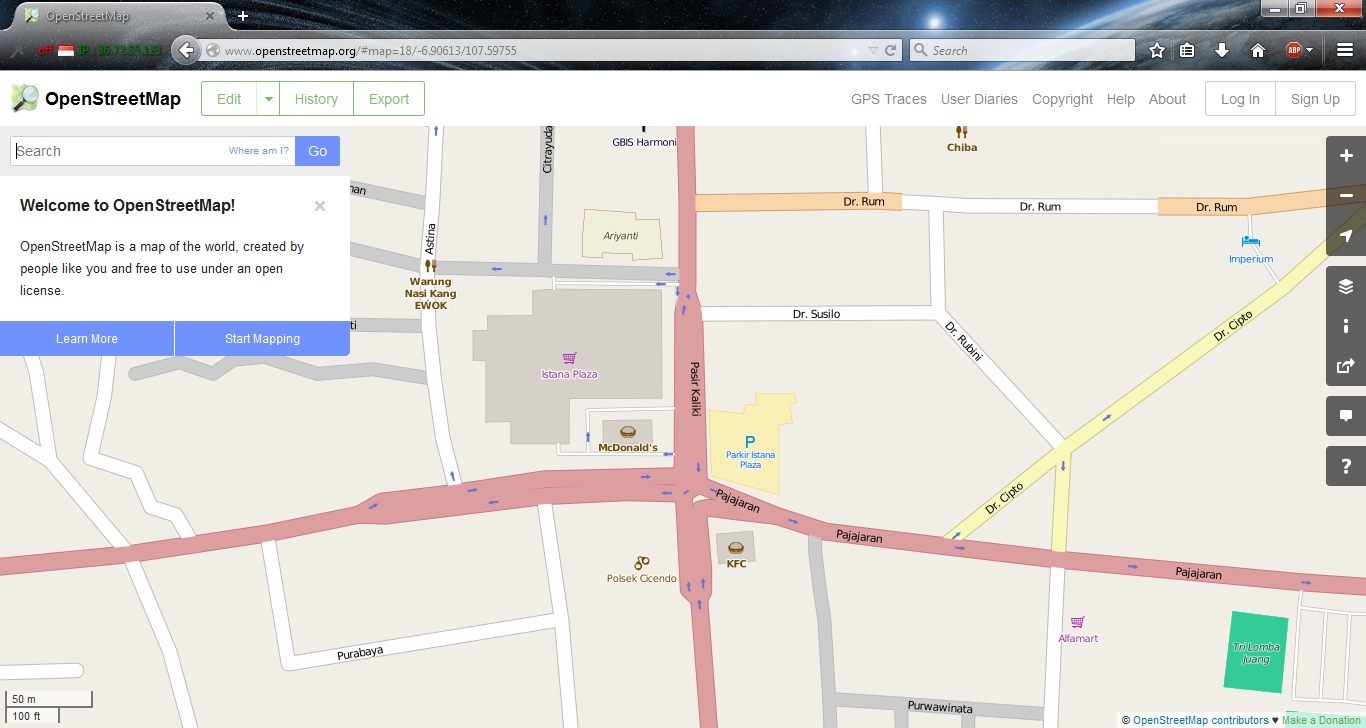
\includegraphics[scale=0.3]{Gambar/web_osm}
\caption[Tampilan website OpenStreetMap]{Tampilan website OpenStreetMap
\footnotemark[1]}
\label{fig:web_osm}
\end{figure}
\footnotetext[1]{http://www.openstreetmap.org}Data yang
disediakan oleh OpenStreetMap dalam bentuk XML biasa disebut
dengan OpenStreetMap XML dan disingkat menjadi OSMXML. OSMXML adalah dokumen XML
yang berisi data-data peta OSM. Pada dasarnya, OSMXML berisi data primitif
(node, way, dan relation) yang merupakan arsitektur dari model OSM. Node
dapat diartikan sebagai titik pada peta dijital, way merupakan informasi garis
pada peta yang melambangkan jalan atau elemen lain seperti rel kereta, dan
relation memberikan informasi node-node yang bersinggungan, elemen
relation dapat menggambarkan suatu area seperti lapangan, taman bermain, rute
bus, dan lain-lain. Sedangkan algoritma Dijkstra
adalah algoritma untuk mencari jarak terpendek antara 2 node pada sebuah graf
berarah dengan bobot yang bernilai tidak negatif pada setiap sisinya \cite{Cormen:2001}. Graf adalah himpunan objek yang terdiri dari simpul(node)
dan sisi (edge), graf dapat digambarkan sebagai kumpulan simpul yang dihubungkan
oleh garis.
Contoh graf dapat dilihat pada Gambar \ref{fig:co_graf}.
\begin{figure}[h]
\centering
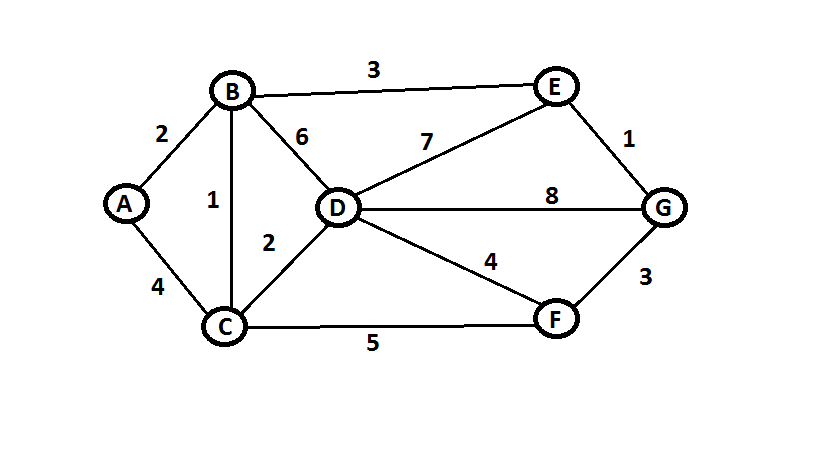
\includegraphics[scale=0.4]{Gambar/co_graf}
\caption[Contoh Graf]{Contoh Graf}
\label{fig:co_graf}
\end{figure}

Aplikasi yang dibangun akan mengolah data yang disediakan oleh OpenStreetMap
dalam bentuk XML dan memodelkannya ke dalam bentuk graf. Selanjutnya akan diimplementasikan algoritma
Dijkstra untuk mencari rute terdekat pada graf tersebut dan menunjukkan hasilnya secara visual.

\section{Rumusan Masalah}
Berdasarkan latar belakang, maka muncul rumusan masalah berikut: 
\begin{itemize}
	\item Bagaimana cara memodelkan data OSMXML menjadi sebuah graf?
	\item Bagaimana cara menggunakan atau mengimplementasikan algoritma Dijkstra
	pada sebuah graf untuk mencari rute terdekat?
	\item Bagaimana cara membuat visualisasi graf dan rute terdekat pada peta
	dijital?
\end{itemize}

\section{Tujuan}
Berdasarkan rumusan masalah yang telah diuraikan di atas, maka tujuan dari penelitian yang dilakukan
adalah:
\begin{itemize} 
	\item Mengetahui cara memodelkan data OSMXML menjadi sebuah	graf.
	\item Mempelajari cara kerja algoritma Dijkstra dan	mengimplementasikannya pada
	sebuah graf.
 	\item Mempelajari cara membuat visualisasi graf dan rute terdekat pada peta
 	dijital.
 \end{itemize}

\section{Batasan Masalah}
Batasan permasalahan dari pembuatan aplikasi ini adalah :
\begin{itemize}
	\item Aplikasi tidak mencari rute terdekat kedua dan seterusnya.
	
	\item Peta hanya menampilkan rute terdekat di wilayah Kota Bandung.
	
	\item Aplikasi tidak memperhitungkan faktor kemacetan jalan.
\end{itemize}

\section{Metodologi Penelitian}
Langkah-langkah yang akan dilakukan dalam melakukan penelitian adalah :
\begin{enumerate}
	\item Melakukan studi pustaka untuk mengetahui teori-teori yang dapat mendukung
	proses pembuatan aplikasi pencarian rute terdekat.
	\item Melakukan analisis teori-teori yang mendukung proses pembuatan aplikasi.
	\item Membuat rancangan aplikasi.
	\item Melakukan implementasi berdasarkan rancangan yang telah dibuat.
	\item Melakukan pengujian aplikasi.
	\item Melakukan pengambilan kesimpulan berdasarkan analisis dan pengujian yang
	telah dilakukan.
\end{enumerate}

\section{Sistematika Pembahasan}
Pada setiap bab akan dibahas beberapa hal sebagai berikut :
\begin{enumerate}
	\item Bab Pendahuluan\\
	Bab 1 berisi latar belakang, rumusan masalah, tujuan, batasan masalah, metodologi penelitian, dan sistematika pembahasan.
	
	\item Bab Dasar Teori\\
	Bab 2 berisi teori-teori dasar mengenai OpenStreetMap, algoritma Dijkstra,
	Google Map Api, Graf, XML, dan beberapa teori lain yang mendukung pembuatan
	aplikasi.
	
	\item Bab Analisis\\
	Bab 3 berisi deskripsi sistem yang akan dibuat, analisis dasar teori, dan
	analisis cara kerja algoritma Dijkstra pada graf.
	
	\item Bab Perancangan\\
	Bab 4 berisi perancangan antarmuka aplikasi disertai beberapa gambar,
	perancangan kelas, dan diagram sekuens.
	
	\item Bab Implementasi dan Pengujian\\
	Bab 5 berisi laporan hasil implementasi yang dilakukan disertai dokumentasi
	mengenai penjelasan aplikasi tersebut dan hasil pengujian yang dilakukan berupa
	\textit{screenshot}
	
	\item Bab Kesimpulan dan Saran\\
	Bab 6 berisi kesimpulan dari seluruh hasil penelitian dan saran untuk
	pengembangan aplikasi yang akan datang.
\end{enumerate}}{}
\ifdefstring{\vbabb}{1}{\chapter{Dasar Teori}
\section{OpenStreetMap}
OpenStreetMap (OSM) adalah portal peta terbuka yang menyediakan data dalam
bentuk peta atau XML \cite{osm}. OSM menyediakan peta dijital dan dapat diedit dari seluruh dunia, juga memungkinkan pengguna untuk mengakses gambar peta yang terdapat pada
situs \url{www.openstreetmap.org} secara gratis. OSM terbentuk dan mendapatkan
datanya dari berbagai sukarelawan yang bersedia untuk berkontribusi, misalnya para pengguna OSM yang menggunakan aplikasi untuk 
mengedit peta dan mengunggah data yang telah diedit ke situs OSM. Selain itu, OSM menyediakan 
beberapa aplikasi bagi para pengguna untuk mengedit peta, seperti iD online editor dan JOSM. 
Untuk mendapatkan gambar peta ataupun data peta dalam bentuk lain, pengguna dapat menggunakan 
fitur export pada situs OSM. Fitur export pada situs OSM dapat
dilihat pada Gambar \ref{fig:export_osm}.
\begin{figure}[h]
\centering
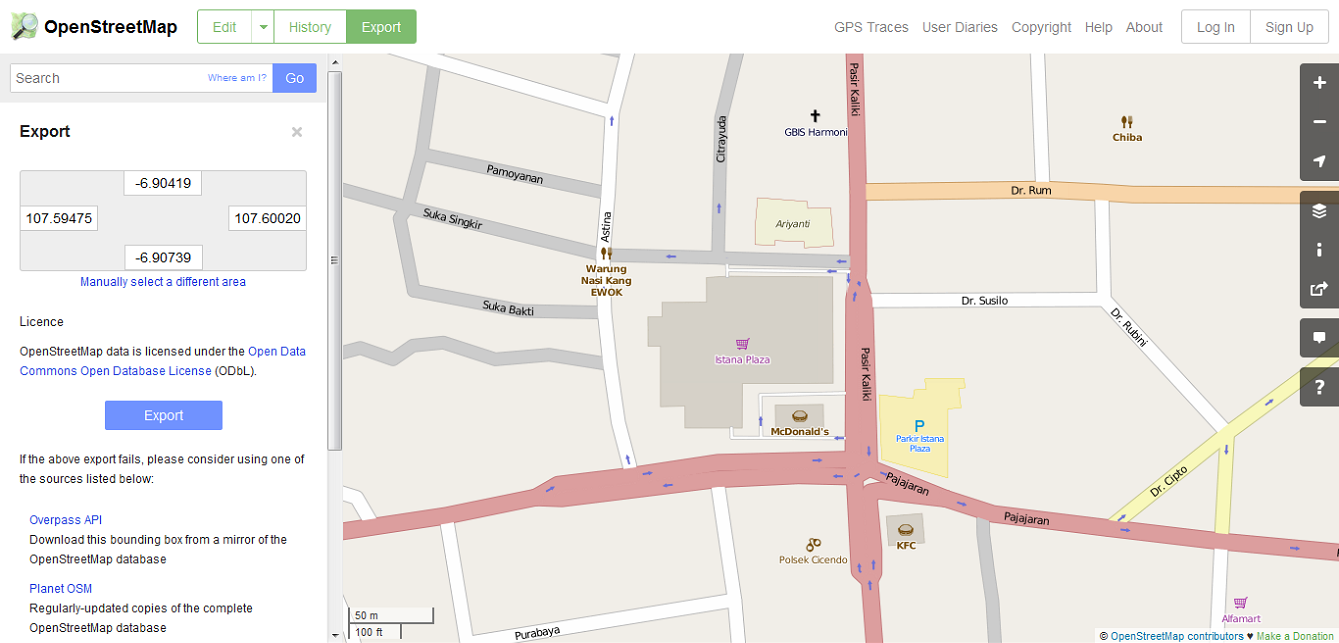
\includegraphics[scale=0.4]{Gambar/export_osm}
\caption[Ekspor data pada situs OpenStreetMap]{Ekspor data pada situs
OpenStreetMap}
\label{fig:export_osm}
\end{figure}

Berikut ini adalah beberapa data yang dapat diambil menggunakan fitur export
\cite{osm}:
\begin{enumerate}
\item OpenStreetMap XML Data

OSM XML data dapat diperoleh dengan cara menggunakan tombol Export di bagian atas untuk 
membuka sidebar. Tombol Export mengarahkan langsung browser kepada OpenStreetMap API yang 
menyediakan data mentah OSM dalam bentuk XML.

\item Mapnik \textit{Image} 

Memungkinkan ekspor data OSM dalam bentuk PNG, JPEG, SVG, PDF dan peta PostScript.

\item \textit{Embeddable} HTML

Fitur ini memungkinkan pengguna untuk mendapatkan kode HTML yang dapat disalin dan digunakan pada halaman web lain. Kode HTML tersebut akan menyisipkan peta dalam sebuah iframe lengkap dengan javascript.
\end{enumerate}

\section{XML}
XML adalah singkatan dari eXtensible Markup Language, XML adalah bahasa markup 
yang dikembangkan oleh W3C (World Wide Web Consortium)
\cite{Benoit:2000}. Berikut ini adalah contoh dokumen XML:
\lstset{basicstyle=\normalsize}
\begin{lstlisting}
<?xml version="1.0" encoding="utf-8"?>
  <catalog>
   <book id="bk101">
      <author>Gambardella, Matthew</author>
      <title>XML Developer's Guide</title>
      <genre>Computer</genre>
      <price>44.95</price>
      <publish_date>2000-10-01</publish_date>
      <description>An in-depth look at creating applications 
      with XML.</description>
   </book>
   <book id="bk102">
      <author>Ralls, Kim</author>
      <title>Midnight Rain</title>
      <genre>Fantasy</genre>
      <price>5.95</price>
      <publish_date>2000-12-16</publish_date>
      <description>A former architect battles corporate zombies, 
      an evil sorceress, and her own childhood to become queen 
      of the world.</description>
   </book>
  <catalog>
\end{lstlisting}
Contoh di atas memberikan informasi mengenai katalog buku yang disimpan pada
dokumen XML. Pada awal dokumen tertera versi XML dan \textit{encoding} yang
digunakan. Setelah itu, terdapat tag catalog yang memiliki \textit{child} yaitu
tag buku beserta informasinya. Terdapat informasi id buku yang tertera pada atribut tag buku,
seperti <book id="bk101">. Dan juga informasi lain seperti judul buku, penulis,
genre, harga, tanggal terbit, dan deskripsi.

XML dikembangkan terutama 
untuk mengatasi keterbatasan pada HTML (Hypertext Markup Language). HTML adalah 
salah satu bahasa markup yang paling populer dan terus dikembangkan, banyak tag baru 
yang diperkenalkan. Pada versi pertama, HTML memiliki satu lusin tag dan pada
HTML pada versi 4.0 sudah hampir mencapai seratus tag. Namun, pada aplikasi
seperti \textit{electronic commerce} dibutuhkan tag lebih untuk produk, harga, nama,
alamat, dan banyak lagi atau situs \textit{streaming} memerlukan tag lebih untuk
mengontrol gambar dan suara.
\lstset{language=XML}

HTML telah berkembang menjadi bahasa yang cukup kompleks, W3C memperkirakan
penggunaan komputer akan terus berkurang dan penggunaan gadget seperti smartphone 
akan bertambah. Mesin tersebut tidak sekuat PC dan tidak bisa memproses bahasa yang 
kompleks seperti HTML . Meskipun HTML adalah bahasa yang populer dan cukup sukses, HTML 
memiliki beberapa kelemahan utama dan XML dikembangkan untuk mengatasi kelemahan tersebut. 
XML adalah bahasa yang digunakan untuk menggambarkan dan memanipulasi dokumen
terstruktur. Perubahan utama pada XML adalah tidak adanya tag yang ditetapkan pada XML. 
Karena tidak ada tag yang ditetapkan, penulis dapat membuat tag yang dibutuhkan. 
Beberapa ketentuan pada XML dapat dilihat pada uraian berikut:
\begin{enumerate}
\item Tag pada XML \\
Setiap elemen pada XML terdiri dari nama dan nilai, selain itu harus memiliki
tag pembuka dan tag penutup. Contoh: 
\begin{verbatim}
<tel> 513-555-7098 </ tel>
\end{verbatim}
Elemen untuk menyimpan nomor telepon memiliki nama tag tel, ditulis dengan <tel>
dan ditutup dengan </tel>.

\item Nama pada XML \\
Pemberian nama pada XML harus dimulai dengan huruf atau underscore (\_) dan
sisanya diikuti huruf, angka, atau titik. Spasi tidak diperbolehkan pada
pemberian nama.

\item Atribut \\
Atribut memungkinkan untuk menyisipkan informasi tambahan, atribut juga memiliki
nama dan nilai. Contoh:
\begin{verbatim}
<tel preferred="true">513-555-8889</tel>
<tel>513-555-7098</tel>
\end{verbatim}
Elemen tel dapat memiliki atribut \textit{preferred}, memberikan informasi nomor
telepon yang lebih sering digunakan.

\item Elemen Kosong \\
Elemen yang tidak memiliki nilai atau isi disebut sebagai elemen kosong. Elemen
kosong biasanya memiliki atribut. Contoh:
\begin{verbatim}
<email href="mailto:jdoe@emailaholic.com"></email>
\end{verbatim}
Elemen email tidak memiliki nilai atau isi.

\item \textit{Nesting of Elements} \\
Sebuah elemen dapat memiliki elemen lain di dalamnya. Elemen yang berada di
dalam elemen lain disebut \textit{child}, sedangkan elemen yang memiliki elemen
lain disebut \textit{parent}. Contoh
\begin{verbatim}
<name>
  <fname>Jack</fname>
  <lname>Smith</lname>
</name>
\end{verbatim}
Pada contoh berikut elemen name memiliki dua
\textit{child} yaitu fname dan lname dan elemen name merupakan \textit{parent}
dari kedua elemen tersebut.

\item \textit{Root} \\
\textit{Root} merupakan elemen level tertinggi, pada dokumen XML harus
ada satu elemen pada level tertinggi. Dengan kata lain, elemen lain harus menjadi
\textit{child} dari \textit{root}.

\item Deklarasi XML \\
Deklarasi XML dituliskan pada baris pertama dokumen. Pada deklarasi tersebut
juga dituliskan versi XML yang digunakan. Contoh:
\begin{verbatim}
<?xml version="1.0"?>
\end{verbatim}
\end{enumerate}

\subsection{OSMXML} \label{ssec:osmxml}
OpenStreetMap XML atau biasa disingkat dengan OSMXML merupakan dokumen XML yang
berisi data-data peta OSM. Pada dasarnya, OSMXML berisi data primitif
(node, way, dan relation) yang merupakan arsitektur dari model OSM
\cite{osm}.
Berikut ini adalah contoh dokumen OSMXML:
\lstset{
  language=XML,
  morekeywords={osm,bounds,node,way,relation,tag,nd,member}
}
\begin{lstlisting}
<?xml version="1.0" encoding="UTF-8"?>
<osm version="0.6" generator="CGImap 0.0.2">
 <bounds minlat="54.0889580" minlon="12.2487570" maxlat="54.0913900" maxlon="12.2524800"/>
 <node id="298884269" lat="54.0901746" lon="12.2482632" user="SvenHRO" uid="46882" visible="true" version="1" changeset="676636" timestamp="2008-09-21T21:37:45Z"/>
 <node id="261728686" lat="54.0906309" lon="12.2441924" user="PikoWinter" uid="36744" visible="true" version="1" changeset="323878" timestamp="2008-05-03T13:39:23Z"/>
 <node id="1831881213" version="1" changeset="12370172" lat="54.0900666" lon="12.2539381" user="lafkor" uid="75625" visible="true" timestamp="2012-07-20T09:43:19Z">
  <tag k="name" v="Neu Broderstorf"/>
  <tag k="traffic_sign" v="city_limit"/>
 </node>
 ...
 <node id="298884272" lat="54.0901447" lon="12.2516513" user="SvenHRO" uid="46882" visible="true" version="1" changeset="676636" timestamp="2008-09-21T21:37:45Z"/>
 <way id="26659127" user="Masch" uid="55988" visible="true" version="5" changeset="4142606" timestamp="2010-03-16T11:47:08Z">
  <nd ref="292403538"/>
  <nd ref="298884289"/>
  ...
  <nd ref="261728686"/>
  <tag k="highway" v="unclassified"/>
  <tag k="name" v="Pastower Straße"/>
  <tag k="oneway" v="yes"/>
 </way>
 <relation id="56688" user="kmvar" uid="56190" visible="true" version="28" changeset="6947637" timestamp="2011-01-12T14:23:49Z">
  <member type="node" ref="294942404" role=""/>
  ...
  <member type="node" ref="364933006" role=""/>
  <member type="way" ref="4579143" role=""/>
  ...
  <member type="node" ref="249673494" role=""/>
  <tag k="name" v="Küstenbus Linie 123"/>
  <tag k="network" v="VVW"/>
  <tag k="operator" v="Regionalverkehr Küste"/>
  <tag k="ref" v="123"/>
  <tag k="route" v="bus"/>
  <tag k="type" v="route"/>
 </relation>
 ...
</osm>
\end{lstlisting}
Struktur OSMXML:
\begin{itemize}
\item Dokumen OSMXML diawali dengan tag xml yang menjelaskan versi xml dan
encoding yang digunakan, pada contoh di atas digunakan xml versi 1.0 dan
encoding UTF-8.

\item Elemen osm memberikan informasi mengenai versi API dan generator yang
digunakan. Generator adalah alat untuk membuat dokumen OSMXML pada saat fitur
export digunakan. 

\item Elemen bound memberikan informasi mengenai cakupan area pada dokumen
OSMXML tersebut. Dilengkapi dengan atribut koordinat yaitu latitude dan longitude.
Data primitif pada OSM dibagi menjadi 3 bagian, yaitu node, way, dan relation.
\begin{enumerate}
\item Elemen Node merupakan informasi titik pada sebuah peta. Node memiliki
beberapa atribut yaitu:
\begin{itemize}
\item id \\
Merupakan id dari node tersebut.

\item user \\ 
Merupakan user yang melakukan editing pada node.

\item uid \\
Id dari user.

\item lat \\
berisi informasi koordinat pada garis lintang.

\item lon \\
berisi informasi koordinat pada garis bujur.

\item timestamp \\
Berisi informasi waktu saat node tersebut diperbaharui.
\end{itemize}
Node juga memiliki elemen tag sebagai \textit{child} yang memberikan informasi
tambahan pada node tersebut, contoh:
\begin{verbatim}
<tag k="name" v="Neu Broderstorf"/>
\end{verbatim}
nama dari node tersebut adalah Neu Broderstorf.

\item Elemen Way merupakan informasi garis yang dapat diartikan sebagai jalan
ataupun elemen lain seperti rel kereta pada peta OSM. Way menyimpan informasi
node-node terurut yang dilalui oleh garis dan juga sama seperti node dilengkapi
atribut seperti id, uid, user, changeset, timestamp. Elemen way memiliki \textit{child}
elemen nd, contoh:
\begin{verbatim}
<nd ref="292403538"/>
\end{verbatim}
atribut ref pada elemen nd mengacu pada node yang memiliki id 292403538, dan
elemen tag yang memberikan informasi tambahan pada elemen way. Selain itu,
elemen way memiliki informasi lain yang disimpan pada elemen tag, elemen tag
merupakan \textit{child} dari elemen way dan menyimpan informasi jenis jalan
yaitu \textit{key highway} dan \textit{key oneway} yang memberikan informasi
arah jalan, contoh:
\begin{verbatim}
<tag k="highway" v="unclassified"/>
<tag k="oneway" v="yes"/>
\end{verbatim}
\textit{Key oneway} memiliki 4 jenis \textit{value}. Informasi arah jalan
mengikuti node-node yang telah terurut. Berikut ini adalah
penjelasan dari keempat \textit{value} tersebut:
\begin{itemize}
  \item oneway=yes \\
  Menunjukkan jalan satu arah
  
  \item oneway=no \\
  Menujukkan jalan dua arah
  
  \item oneway=-1 \\
  Menunjukkan jalan satu arah dan berlawanan
  
  \item oneway=reversible \\
  Menunjukkan jalan satu arah dan dapat berubah arah menjadi berlawanan. Contoh,
  pengalihan jalan untuk mengatasi kemacetan.
\end{itemize}

\item Elemen relation menyimpan informasi node-node dan way yang bersinggungan.
Elemen relation dapat menggambarkan suatu area seperti lapangan, taman bermain, atau
pada contoh di atas menggambarkan rute bus.
\end{enumerate}
\end{itemize}

\section{Javascript}
Javascript adalah bahasa pemrograman web yang mulai dikembangkan di perusahaan
yang bernama Netscape. Javascript memiliki lisensi dari Sun Microsystems yang sekarang sudah berganti nama 
menjadi Oracle. Saat ini, mayoritas situs web sudah menggunakan javascript.
Berikut ini adalah contoh penggunaan javascript pada dokumen HTML:
\lstset{
  language=HTML
}
\begin{lstlisting}
<!DOCTYPE html>
<html>
<head>
<script>
function myFunction() {
    document.getElementById("demo").innerHTML = "Paragraph changed.";
}
</script>
</head>
<body>
<h1>JavaScript in Head</h1>
<p id="demo">A Paragraph.</p>
<button type="button" onclick="myFunction()">Try it</button>
</body>
</html> 
\end{lstlisting}
Pada contoh di atas terdapat fungsi yang ditulis menggunakan javascript,
fungsi tersebut akan mengubah string ``A Paragraph'' pada tag <p> menjadi
``Paragraph changed'' jika \textit{button} atau tombol ``Try it'' di klik.

Seluruh browser yang terdapat pada komputer, konsol game, tablet, dan smartphone
sudah disertai dengan javascript interpreter. Interpreter adalah suatu program yang berfungsi 
untuk menerjemahkan kode program ke dalam bahasa mesin. Javascript adalah bagian yang 
cukup penting pada sebuah halaman web, jika HTML 
berfungsi untuk menentukan isi dari halaman dan CSS untuk menentukan tampilan pada halaman, javascript 
berfungsi untuk menentukan ``behavior'' dari halaman web tersebut
\cite{Flanagan:2011}.
Berikut ini adalah uraian dari struktur javascript dan beberapa contoh sintaks:
\begin{enumerate}
\item Struktur

\begin{itemize}
\item \textit{Character Set} \\
Javascript ditulis menggunakan karakter Unicode. Unicode adalah superset ASCII dan Latin-1 yang mendukung 
hampir seluruh bahasa di dunia.

\item \textit{Comments} \\
Javascript mendukung 2 jenis komentar yaitu komentar yang diletakkan setelah garis miring ganda // dan komentar yang 
diletakkan antara karakter /* dan */.
\begin{verbatim}
// This is a single-line comment.
/* This is also a comment */ // and here is another comment.
/*
* This is yet another comment.
* It has multiple lines.
*/
\end{verbatim}

\item Literal \\
Literal adalah notasi untuk merepresentasikan nilai 
dan nilai yang dituliskan akan muncul secara langsung dalam program. Literal
dapat berupa karakter, bilangan bulat, bilangan real, boolean. Berikut
ini adalah contoh literal:
\begin{verbatim}
12 // The number twelve
1.2 // The number one point two
"hello world" // A string of text
'Hi' // Another string
true // A Boolean value
false // The other Boolean value
/javascript/gi // A "regular expression" literal (for pattern matching)
null // Absence of an object 
\end{verbatim}

\item \textit{Identifier} \\
\textit{Identifier} pada javascript hanyalah nama yang digunakan untuk memberi
nama pada variabel atau fungsi. Digit tidak diperbolehkan sebagai karakter
pertama pada \textit{identifier}.

\item \textit{Reserved words} \\
\textit{Reserved words} adalah kata-kata yang tidak dapat digunakan sebagai
identifier, karena digunakan oleh javascript sebagai keyword. Beberapa contoh keyword seperti break, delete, if, 
null, true, false, try, dan lain-lain.

\item \textit{Optional Semicolons} \\
Seperti banyak bahasa pemrograman lain, javascript menggunakan titik koma (;) untuk memisahkan perintah 
yang ditulis. Hal ini penting untuk membuat kode program menjadi jelas mengenai awal dan akhir. Pada 
javascript, titik koma dapat dihilangkan jika perintah ditulis pada baris yang berbeda, berikut adalah 
contoh penggunaan titik koma pada javascript:
\begin{verbatim}
a = 3;
b = 4;
\end{verbatim}
titik koma pertama dapat dihilangkan, namun jika ditulis pada baris yang sama, titik koma tetap diperlukan
\begin{verbatim}
a = 3; b = 4;
\end{verbatim}
\end{itemize}

\item Sintaks
\begin{itemize}
\item Deklarasi Variabel \\
Pembuatan variabel pada javascript menggunakan keyword var. Contoh deklarasi atau pembuatan variabel pada javascript:
\begin{verbatim}
var i;
var i, sum;
var message = "hello";
var i = 0, j = 0, k = 0;
\end{verbatim}


\item Fungsi \\
Fungsi adalah blok kode program yang hanya didefinisikan sekali, tapi dapat
dipanggil atau dijalankan berulang kali. Pada javascript, fungsi dapat dibuat menggunakan keyword function. 
Sebuah fungsi harus memiliki nama, sepasang tanda kurung untuk parameter, dan sepasang kurung kurawal. 
Berikut ini adalah beberapa contoh fungsi:
\begin{verbatim}
// Print the name and value of each property of o. Return undefined.
function printprops(o) {
  for(var p in o)
    console.log(p + ": " + o[p] + "\n");
}
\end{verbatim}
\begin{verbatim}
// Compute the distance between Cartesian points (x1,y1) and (x2,y2).
function distance(x1, y1, x2, y2) {
  var dx = x2 - x1;
  var dy = y2 - y1;
  return Math.sqrt(dx*dx + dy*dy);
}
\end{verbatim}
\end{itemize}
\end{enumerate}

\subsection{XMLHttpRequest}
XMLHttpRequest adalah salah satu objek pada javascript yang dapat digunakan
untuk mendapatkan \textit{file} XML dari \textit{server} secara \textit{asynchronous}
atau \textit{synchronous} \cite{Edmond:2006}. \textit{Asynchronous} berarti
bahwa pertukaran data dilakukan tanpa harus memuat ulang seluruh halaman \textit{web}, sedangkan 
pertukaran data \textit{synchronous} harus memuat ulang seluruh halaman
\textit{web}. Berikut ini adalah contoh penggunaan XMLHttpRequest:
\begin{verbatim}
var objXMLHTTP = new XMLHttpRequest();

objXMLHTTP.open('GET', 'books.xml', false);
objXMLHTTP.send(null);

var objXML = objXMLHTTP.responseXML;
\end{verbatim}
Langkah pertama adalah dengan membuat objek XMLHttpRequest. Selanjutnya, dengan
memanggil fungsi open(``method'', ``url'', asynchronous). Parameter
\textit{method} menentukan metode yang digunakan, contoh ``GET'' untuk menerima
data dan ``POST'' untuk mengirim data, parameter url adalah alamat
\textit{file}, dan parameter boolean ``false'' menunjukkan bahwa permintaan tersebut
dilakukan secara \textit{synchronous}. Langkah terakhir adalah mendapatkan
respon dari \textit{server}. Berikut ini penjelasan dari setiap \textit{method}
yang digunakan:
\begin{enumerate}
  \item open("method","url", asynchronous,"username","password")\\
  Melakukan inisialisasi permintaan\\
	Parameter:
  \begin{itemize}
    \item \textit{method}\\
    Method pada HTTP yang digunakan seperti ``GET'' dan ``POST''.
    
    \item \textit{url}\\
    Alamat url tujuan 
    
    \item \textit{asynchronous}\\
    boolean Opsional, secara default bernilai \textit{true}. \textit{True}
    menyatakan bahwa operasi yang dijalankan secara \textit{asynchronous}. Nilai
    \textit{false} menyatakan sebaliknya.
    
    \item \textit{username}\\
    Opsional, berisikan \textit{username} yang digunakan untuk keperluan
    otentikasi.
    Secara default, berisi string kosong.
    
    \item \textit{password}\\
    Opsional, berisikan \textit{password} yang digunakan untuk keperluan
    otentikasi. Secara default, berisi string kosong.
  \end{itemize}
  
  \item send(content)\\
  Mengirimkan permintaan\\
  Parameter:
  \begin{itemize}
    \item \textit{content}\\
    Opsional, \textit{content} dapat berisi string atau data lainnya seperti
    Array, dokumen, dan lain-lain.
  \end{itemize}
  
  \item responseXML\\
  Respon dari permintaan\\
  Return:\\
  DOM Object
\end{enumerate}

\subsection{XML DOM}
DOM adalah singkatan dari \textit{Document Object Model}, XML DOM adalah API
umum untuk menangani dokumen XML \cite{Edmond:2006}. API adalah singkatan dari
\textit{Application Programming Interface} merupakan fungsi atau perintah yang dapat digunakan untuk
menangani masalah pemrograman tertentu. XML DOM menyediakan fungsi standar
untuk mengakses, memodifikasi, dan menciptakan berbagai bagian dari sebuah dokumen XML.
Contoh:
\begin{verbatim}
var myNodeset = objXML.getElementsByTagName('plant');
var name = myNodeset[0].getAttribute('name');
\end{verbatim}
Pemanggilan fungsi getElementsByTagName('plant') akan mengembalikan satu set
node yang memiliki nama tag 'plant'. Contoh lain, pemanggilan fungsi
getAttribute() akan mengembalikan nilai atribut. Berikut ini penjelasan dari 
setiap \textit{method} yang digunakan:
\begin{enumerate}
  \item getElementsByTagName('tagName')\\
  Mengembalikan elemen-elemen yang memiliki kesesuaian nama.\\
  Parameter:
  \begin{itemize}
    \item tagName\\
    String yang menentukan nama elemen yang dicari.
  \end{itemize}
  Return:\\
  objek berisi elemen yang memiliki nama sesuai dengan yang dicari.
  
  \item getAttribute('name')\\
  Mengembalikan nilai atribut\\
  Parameter:
  \begin{itemize}
    \item name\\
    String yang menentukan nama atribut yang dicari.
  \end{itemize}
  Return:\\
  Mengembalikan string jika atribut memiliki nilai, jika tidak mengembalikan
  \textit{null}.
\end{enumerate}


\subsection{Google Maps Javascript API}
Google Maps Javascript API memungkinkan untuk sebuah halaman web menampilkan
peta dunia yang datanya didapat dari server google \cite{gmap}. Google
menyediakan fungsi atau perintah untuk menampilkan dan menyesuaikan peta sesuai dengan
kebutuhan. 
\setcounter{secnumdepth}{3}
\setcounter{tocdepth}{3}
\subsubsection{Elemen Dasar Google Maps}
Google Maps Javascript API menyediakan fungsi dan kelas untuk memuat sebuah peta
pada halaman html. Berikut ini adalah contoh halaman web yang menampilkan peta
di lokasi Sydney, Australia:
\lstset{
  language=HTML
}
\begin{lstlisting}
<!DOCTYPE html>
<html>
  <head>
    <style type="text/css">
      html, body, #map-canvas { height: 100%; margin: 0; padding: 0;}
    </style>
    <script type="text/javascript"
      src="https://maps.googleapis.com/maps/api/js?key=API_KEY">
    </script>
    <script type="text/javascript">
      function initialize() {
        var mapOptions = {
          center: { lat: -34.397, lng: 150.644},
          zoom: 8
        };
        var map = new google.maps.Map(document.getElementById('map-canvas'),
            mapOptions);
      }
      google.maps.event.addDomListener(window, 'load', initialize);
    </script>
  </head>
  <body>
<div id="map-canvas"></div>
  </body>
</html>
\end{lstlisting}
\begin{itemize}
\item Declaring \\
Google menyarankan untuk membuat deklarasi tipe dokumen pada awal dokumen yaitu
dengan menulis <!DOCTYPE html>. Setelah itu diperlukan CSS yang bekerja untuk
mengatur tampilan peta pada halaman web.
\begin{verbatim}
<style type="text/css">
  html { height: 100% }
  body { height: 100%; margin: 0; padding: 0 }
  #map-canvas { height: 100% }
</style>
\end{verbatim}
Kode CSS pada contoh menunjukkan tag yang memiliki id map-canvas akan memiliki
tinggi 100\% pada saat ditampilkan dan juga menunjukkan persentase yang sama
pada <html> dan <body>.

\item Loading Google Maps API\\
Untuk dapat menampilkan peta diperlukan juga melakukan \textit{load} javascript.
URL yang terdapat pada tag script adalah lokasi file javascript yang akan memuat
seluruh simbol dan definisi yang dibutuhkan untuk menggunakan Google Maps API
ini. Paramater key berisi API key yang dimiliki oleh pengguna.
\begin{verbatim}
<html>
  <head>
    <script type="text/javascript"
      src="https://maps.googleapis.com/maps/api/js?key=API_KEY">
    </script>
\end{verbatim}

\item Initialize \\
Setelah melakukan load javascript, diperlukan pemanggilan fungsi initialize. Di
dalam fungsi tersebut dapat ditambahkan beberapa variabel yang dibutuhkan.
\begin{verbatim}
function initialize() {}
\end{verbatim}
Untuk inisialisasi peta, diperlukan variabel \textit{map options}
\begin{verbatim}
var mapOptions = {};
\end{verbatim}
Selanjutnya diperlukan koordinat pusat peta yang akan ditampilkan, sedangkan
zoom menunjukkan level zoom yang ingin ditampilkan
\begin{verbatim}
center: new google.maps.LatLng(-34.397, 150.644),
zoom: 8
\end{verbatim}

\item Map Object \\
objek peta perlu dibuat dengan cara melakukan inisialisasi kelas
google.maps.Map. Pada contoh, peta diletakkan pada <div> yang memiliki id
map-canvas.
\begin{verbatim}
var map = new google.maps.Map(document.getElementById("map-canvas"),
    mapOptions);
\end{verbatim}

\item Loading the Map \\
Google Maps API menyediakan fungsi untuk memuat peta. Pada potongan kode
di bawah, fungsi \textit{listener} akan memanggil fungsi \textit{initialize}
ketika halaman dimuat.
\begin{verbatim}
google.maps.event.addDomListener(window, 'load', initialize);
\end{verbatim}
\end{itemize}
Berikut ini adalah penjelasan kelas dan fungsi yang digunakan:
\begin{enumerate}
  \item google.maps.Map class\\
  Membuat peta baru pada halaman html.\\
  Konstruktor:
  \begin{itemize}
    \item mapDiv:Node\\
    node yang digunakan untuk membuat peta.
    
    \item opts?:MapOptions\\
    Opsi dari \textit{map} yang akan dibuat. 
  \end{itemize}
  
  \item google.maps.LatLng class\\
  Membuat objek Latlng yang merepresentasikan titik geografis.\\
  Konstruktor:
  \begin{itemize}
    \item lat:number\\
    \textit{Latitude} dalam derajat.
    
    \item lng:number\\
    \textit{Longitude} dalam derajat.
    
    \item noWrap?:boolean\\
    \textit{Latitude} ditentukan dalam rentang derajat -90 hingga 90 dan
    \textit{longitude} ditentukan dalam rentang derajat -180 hingga 180. Nilai
    \textit{true} pada boolean noWrap untuk mengaktifkan nilai di luar
    batas tersebut.
  \end{itemize}
  
  \item google.maps.event.addDomListener(instance:Object, eventName:string,
  handler:Function)\\
  Menambahkan fungsi \textit{listener}\\
  Parameter:
  \begin{itemize}
    \item instance:Object\\
    Objek yang ditambahkan \textit{listener}.
    
    \item eventName:string\\
    Nama \textit{Event}.
    
    \item handler:Function\\
    Fungsi yang dipanggil ketika \textit{event} terjadi.
  \end{itemize}
  Return:\\
  MapsEventListener
\end{enumerate}

\subsubsection{Menggambar pada Peta}
Peta pada Google Maps API dapat ditambahkan objek seperti titik, garis, area,
atau objek lainnya. objek tersebut dinamakan \textit{overlay}. Terdapat beberapa
jenis \textit{overlay} yang dapat ditambahkan pada peta yaitu \textit{marker}
dan \textit{polyline}. Berikut ini adalah penjelasan kelas dan fungsi yang
digunakan:
\begin{enumerate}
  \item google.maps.Marker class \\
  Membuat \textit{marker} pada peta dengan opsi tertentu.\\
  Konstruktor:
  \begin{itemize}
    \item opts?:MarkerOptions\\
    Opsi dari \textit{marker} yang dibuat.
  \end{itemize}
  
  \item google.maps.Polyline class\\
  Membuat \textit{polyline} pada peta dengan opsi tertentu.\\
  Konstruktor:
  \begin{itemize}
    \item opts?:PolylineOptions\\
    Opsi dari \textit{polyline} yang dibuat.
  \end{itemize}
  
  \item setMap(map:Map)\\
  Menyisipkan \textit{marker} atau \textit{polyline} pada peta tertentu.\\
  Parameter:
  \begin{itemize}
    \item map:Map\\
    Peta yang disisipkan \textit{marker} atau \textit{polyline}.
  \end{itemize}
  
  \item setIcon(icon:string|Icon|Symbol)\\
  Mengubah \textit{icon} pada \textit{marker}.\\
  Parameter:
  \begin{itemize}
    \item icon:string|Icon|Symbol\\
    \textit{Icon yang digunakan}.
  \end{itemize}
\end{enumerate}

Berikut ini adalah contoh penggunaan \textit{marker} dan \textit{polyline} pada
peta:
\begin{enumerate}
\item \textit{Marker} \\
Lokasi tunggal pada peta ditunjukkan oleh \textit{Marker}.
\begin{itemize}
  \item Menambahkan \textit{Marker} \\
  Untuk menampilkan \textit{marker} pada peta harus membuat objek
  google.maps.Marker. Berikut ini adalah atribut penting pada saat
  membuat objek \textit{marker}:
  \begin{enumerate}
    \item \textit{position} \\
    atribut \textit{position} diperlukan untuk mengatur letak \textit{marker}
    pada peta.
    
    \item \textit{map} \\
    atribut \textit{map} bersifat opsional, untuk menentukan marker
    tersebut akan diletakkan pada peta. Jika atribut \textit{map} tidak diatur,
    maka \textit{marker} akan tetap dibuat tetapi tidak akan ditampilkan pada
    peta.
  \end{enumerate}
  Berikut ini adalah contoh kode program untuk menambahkan \textit{marker} pada
  peta:
\begin{verbatim}
var myLatlng = new google.maps.LatLng(-25.363882,131.044922);
	var mapOptions = {
	  zoom: 4,
	  center: myLatlng
	}
	var map = new google.maps.Map(document.getElementById
	("map-canvas"), mapOptions);
	
	// To add the marker to the map, use the 'map' property
	var marker = new google.maps.Marker({
	    position: myLatlng,
	    map: map,
	    title:"Hello World!"
	});
\end{verbatim}
  Pada contoh, objek google.maps.Marker yang dibuat disimpan pada variabel
  \textit{marker}, terdapat atribut \textit{position} menggunakan variabel
  \textit{myLatlng} yang berisi koordinat (-25.363882,131.044922), atribut map
  menunjukkan bahwa \textit{marker} akan ditampilkan pada objek map yang tersimpan pada variabel
  \textit{map}, dan atribut yang menunjukkan judul \textit{marker}. 
  
  \item Mengubah \textit{icon marker}\\
  Untuk mengubah \textit{icon}, diperlukan pengaturan pada konstruktor
  \textit{marker} tersebut. Pada contoh, \textit{icon marker} diubah
  menjadi beachflag.png.
\begin{verbatim}
  var image = 'images/beachflag.png';
  var myLatLng = new google.maps.LatLng(-33.890542, 151.274856);
  var beachMarker = new google.maps.Marker({
      position: myLatLng,
      map: map,
      icon: image
  });
\end{verbatim}
Selain pengaturan pada kontruktor, pengubahan \textit{icon} juga dapat dilakukan
dengan cara memanggil fungsi setIcon()
\begin{verbatim}
	beachMarkers.setIcon('images/beachflag.png');
\end{verbatim}

  \item Menghapus \textit{Marker} pada peta\\
  Untuk menghapus \textit{marker} pada peta, hanya diperlukan pemanggilan
  fungsi setMap() dan mengisi parameter fungsi tersebut dengan \textit{null}.
  Contoh:
\begin{verbatim}
marker.setMap(null);
\end{verbatim}
  Pada contoh di atas hanya menghilangkan \textit{marker} dari peta dan tidak
  menghapus objek \textit{marker}.
  
  \item Animasi \textit{Marker} \\
  Menambahkan animasi pada \textit{marker}, hanya memerlukan pengaturan atribut
  pada konstruktor google.maps.Marker. Contoh:
\begin{verbatim}
  var marker = new google.maps.Marker({
	    position: myLatlng,
	    map: map,
	    animation: google.maps.Animation.BOUNCE,
	    title:"Hello World!"
	});
\end{verbatim}
  Pada contoh, menambahkan animasi \textit{bounce} pada marker sehingga
  \textit{marker} bergerak melompat-lompat pada peta. 
  
  \item Mengubah Ikon \\
  Gambar \textit{marker} pada peta dapat diubah sesuai keinginan, hanya
  memerlukan pengaturan atribut pada konstruktor google.maps.Marker. Contoh:
\begin{verbatim}
  var image = 'images/beachflag.png';
  var myLatLng = new google.maps.LatLng(-33.890542, 151.274856);
  var beachMarker = new google.maps.Marker({
      position: myLatLng,
      map: map,
      icon: image
  });
\end{verbatim}
  Pada contoh, ikon \textit{marker} akan ditampilkan menggunakan \textit{file}
  gambar beachflag.png
  
  \item \textit{Draggable} \\
  Draggable memungkinkan pengguna untuk menyeret marker ke lokasi yang berbeda,
  hanya memerlukan pengaturan atribut pada konstruktor google.maps.Marker. Contoh:
\begin{verbatim}
  var marker = new google.maps.Marker({
	    position: myLatlng,
	    map: map,
	    draggable: true,
	    title:"Hello World!"
	});
\end{verbatim}
\end{itemize}
\item \textit{Polyline} \\
Objek \textit{polyline} adalah serangkaian garis pada peta, \textit{polyline}
berguna untuk menunjukkan dari satu titik ke titik lain. \textit{Polyline}
memiliki atribut yang dapat diubah sesuai kebutuhan seperti warna,
\textit{opacity}, dan \textit{weight}. Berikut ini penjelasan dari
beberapa atribut tersebut:
\begin{itemize}
  \item \textit{strokeColor} \\
  Atribut \textit{strokeColor} menentukan warna dalam format
  heksadesimal, contoh \\ "\#FFFFFF''.
  
  \item \textit{strokeOpacity} \\
  Atribut \textit{strokeOpacity} menentukan \textit{opacity} dalam nilai antara
  0.0 dan 1.0.
  
  \item \textit{strokeWeight} \\
  Atribut \textit{strokeWeight} menentukan lebar garis dalam piksel.
\end{itemize}
Berikut ini adalah contoh potongan kode program untuk menampilkan
\textit{polyline} pada peta:
\begin{verbatim}
var flightPlanCoordinates = [
    new google.maps.LatLng(37.772323, -122.214897),
    new google.maps.LatLng(21.291982, -157.821856),
    new google.maps.LatLng(-18.142599, 178.431),
    new google.maps.LatLng(-27.46758, 153.027892)
  ];
  var flightPath = new google.maps.Polyline({
    path: flightPlanCoordinates,
    strokeColor: '#FF0000',
    strokeOpacity: 1.0,
    strokeWeight: 2
  });

  flightPath.setMap(map);
\end{verbatim}
Pada contoh, akan menampilkan polyline pada peta yang akan menghubungkan setiap 
koordinat yang terdapat pada variabel \textit{flightPlanCoordinates}.
\textit{Polyline} yang ditampilkan pada peta dapat dilihat pada Gambar \ref{fig:polyline}.
\begin{figure}[h]
\centering
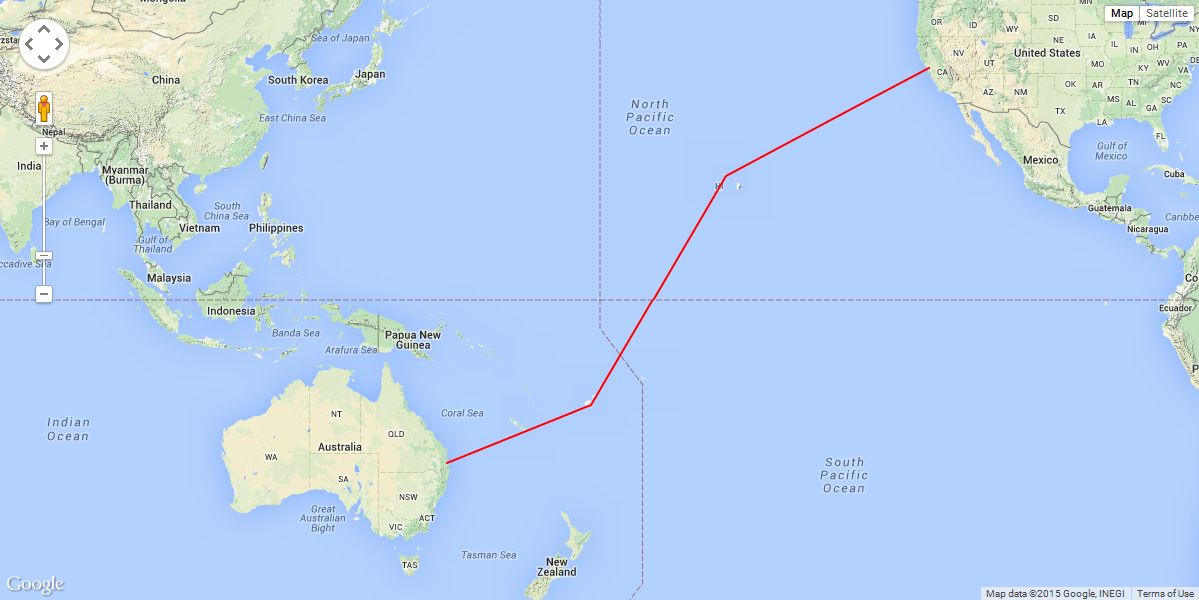
\includegraphics[scale=0.4]{Gambar/polyline}
\caption[Polyline pada Peta]{Polyline pada Peta}
\label{fig:polyline}
\end{figure}
\end{enumerate}

\subsubsection{\textit{Geometry Library}}
Gambar pada Google Maps adalah dua dimensi, sedangkan bumi adalah tiga dimensi
yang menyerupai bentuk bola. Hal ini tentu akan berbeda ketika mengukur suatu
jarak dari satu titik ke titik lain, misalnya jarak terpendek antara dua titik 
pada bola bukanlah garis lurus, tetapi menyerupai lingkaran besar atau busur. 
Karena perbedaan tersebut, diperlukan \textit{spherical geometry} untuk
menghitung data geometris pada permukaan bumi seperti sudut, jarak, dan area 
yang berdasarkan garis lintang dan garis bujur. Google Maps JavaScript API 
menyediakan \textit{geometry library} yang memiliki fungsi utilitas tersebut,
fungsi utilitas tersebut dinamakan google.maps.geometry.spherical. Untuk
menghitung jarak antara dua titik dapat memanggil fungsi
computeDistanceBetween().
\begin{enumerate}
  \item google.maps.geometry.spherical namespace \\
  Fungsi utilitas untuk menghitung sudut, jarak, dan area. Secara
  \textit{default}, radius bumi yang digunakan adalah 6378137 meter.
  
  \item computeDistanceBetween(from:LatLng, to:LatLng, radius?:number) \\
  Menghitung jarak antara dua titik.\\
  Parameter:
  \begin{itemize}
    \item from:LatLng\\
    Koordinat titik pertama.
    
    \item to:LatLng\\
    Koordinat titik kedua.
    
    \item radius?:number\\
    Radius yang digunakan.
  \end{itemize}
\end{enumerate}
Berikut ini adalah contoh penggunaan fungsi computeDistanceBetween() untuk
menghitung jarak antara koordinat Kota Jakarta dan koordinat Kota Bandung:
\begin{verbatim}
var jakarta = new google.maps.LatLng(-6.1745,106.8227);
var bandung = new google.maps.LatLng(-6.9167,107.6000);

var distance = google.maps.geometry.spherical
.computeDistanceBetween(jakarta, bandung);
\end{verbatim}
setelah menggunakan fungsi computeDistanceBetween(), didapatkan jarak antara dua
titik koordinat tersebut adalah 119231.23264342443 meter atau lebih kurang
119,2 kilometer.
 
\subsubsection{\textit{Info Window}}
\textit{Info window} adalah kelas yang disediakan Google Maps untuk menampilkan
konten (biasanya berupa teks atau gambar) pada jendela \textit{popup}.
\textit{Info window} memiliki ujung yang melekat ke lokasi tertentu pada peta.
Biasanya \textit{info window} diletakkan pada \textit{marker} yang ada pada
peta, tetapi \textit{info window} juga dapat diletakkan pada koordinat peta
tertentu. Berikut ini adalah contoh potongan kode program yang menampilkan
\textit{marker} beserta \textit{info window}:
\begin{verbatim}
  var contentString = 'Info Window';

  var infowindow = new google.maps.InfoWindow({
      content: contentString
  });

  var marker = new google.maps.Marker({
      position: myLatlng,
      map: map,
      title: 'Uluru (Ayers Rock)'
  });
  google.maps.event.addListener(marker, 'click', function() {
    infowindow.open(map,marker);
  });
\end{verbatim}
Pada contoh, terdapat variabel \textit{contentString} yang berisi teks yang akan
dimuat pada \textit{info window}. Selanjutnya, diperlukan variabel
\textit{infowindow} yang menginisialisasi \textit{info window} dan variabel
\textit{marker} yang menginisialisasi \textit{marker}. Dan \textit{listener}
yang memanggil fungsi \textit{open} ketika \textit{marker} tersebut diklik.
Berikut ini adalah penjelasan dari kelas dan fungsi yang digunakan:
\begin{enumerate}
\item google.maps.InfoWindow class\\
  Membuat \textit{overlay} yang berbentuk seperti gelembung dan memuat konten
  seperti teks atau gambar.\\
  Konstruktor:
  \begin{itemize}
    \item opts?:InfoWindowOptions\\
    Opsi dari \textit{info window} yang dibuat.
  \end{itemize}
  
\item open(map?:Map|StreetViewPanorama, anchor?:MVCObject)\\
  Membuka info window pada peta.\\
  Parameter
  \begin{itemize}
    \item map?:Map|StreetViewPanorama\\
    Membuka \textit{info window} pada peta yang diberikan.
    
    \item anchor?:MVCObject\\
    Objek yang berasosiasi dengan \textit{info window}, contoh: \textit{marker}.
  \end{itemize}
\end{enumerate}
\textit{Info Window} yang ditampilkan pada peta dapat dilihat pada Gambar
\ref{fig:infowindow}.
\begin{figure}[h]
\centering
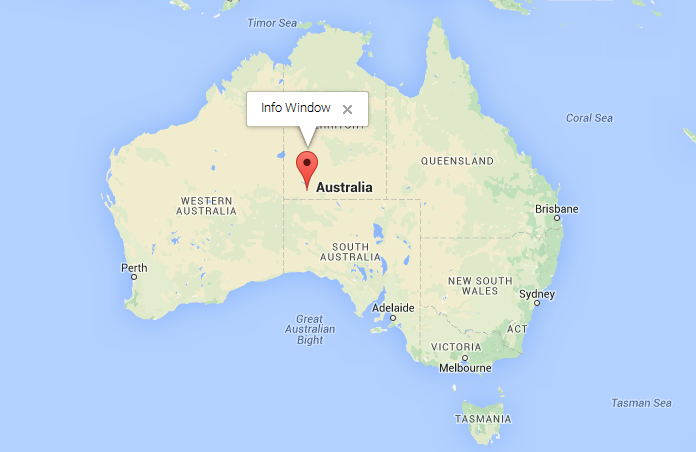
\includegraphics[scale=0.6]{Gambar/infowindow}
\caption[Info Window pada Peta]{Info Window pada Peta}
\label{fig:infowindow}
\end{figure}


\section{Graf}
Graf adalah himpunan objek yang terdiri dari node (simpul) dan edge (sisi), graf 
digambarkan sebagai node yang dihubungkan oleh edge. Terdapat berbagai
macam jenis graf, tetapi pada subbab ini akan dibahas beberapa jenis graf
seperti graf tidak berarah, graf berarah, dan graf berbobot. Contoh graf dapat
dilihat pada Gambar \ref{fig:graph}. Graf mengikuti aturan berikut \footnotemark[2]:
\footnotetext[2]{http://web.cecs.pdx.edu/sheard/course/Cs163/Doc/Graphs.html}
\begin{enumerate}
\item Graf terdiri dari dua bagian yang disebut node dan edge.
\item Node digambarkan berdasarkan tipenya dan nilainya mungkin terbatas atau
tidak terbatas. 
\item Setiap node menghubungkan dua buah edge.
\item Node digambarkan sebagai kotak atau lingkaran dan edge digambarkan sebagai
garis atau busur.
\end{enumerate}

\begin{figure}[h]
\centering
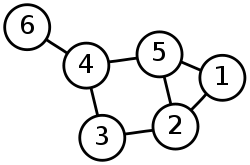
\includegraphics[scale=1]{Gambar/graph}
\caption[Contoh Graf]{Contoh Graf}
\label{fig:graph}
\end{figure}
Berdasarkan contoh pada Gambar \ref{fig:graph}  didapatkan informasi tipe dari
node adalah bilangan bulat \\
Himpunan node = {1,2,3,4,5,6} \\ 
Himpunan edge = {(6,4),(4,5),(4,3),(3,2),(5,2),(2,1),(5,1)}

\subsection{Graf Tidak Berarah}
Graf tidak berarah adalah graf yang tidak memiliki arah pada setiap edgenya,
sehingga setiap node tidak memiliki urutan. Graf tidak berarah digambarkan dengan garis lurus
antara node. Contoh graf berarah dapat dilihat pada Gambar
\ref{fig:graph}.

\subsection{Graf Berarah}
Graf berarah memiliki arah pada setiap edgenya. Pada graf berarah, edge biasanya
digambarkan dengan panah sesuai arahnya. Contoh graf berarah dapat dilihat pada
Gambar \ref{fig:direc_graph}.
\begin{figure}[h]
\centering
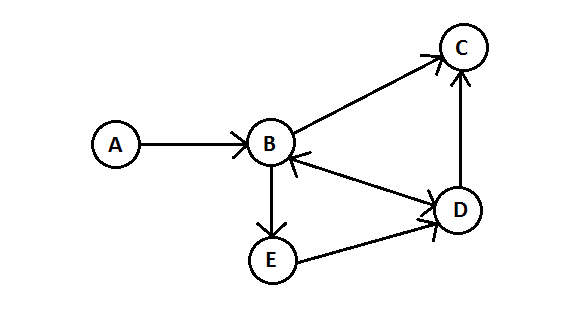
\includegraphics[scale=1]{Gambar/direc_graph}
\caption[Contoh Graf Berarah]{Contoh Graf Berarah}
\label{fig:direc_graph}
\end{figure}
Berdasarkan contoh pada Gambar \ref{fig:direc_graph}  didapatkan informasi tipe
dari node adalah huruf kapital. \\
Himpunan node = {A, B, C, D, E} \\ 
Himpunan edge = {(A, B), (B, C), (D, C), (B, D), (D, B), (E, D), (B, E)}

\subsection{Graf Berbobot}
Graf berbobot adalah graf yang memiliki nilai pada setiap edgenya. Nilai
tersebut dapat berupa bilangan bulat ataupun bilangan pecahan desimal. Nilai
tersebut dapat digunakan untuk menyimpan jarak dari suatu node ke node lain.
Contoh graf berbobot dapat dilihat pada Gambar \ref{fig:weight_graph}.
\begin{figure}[h]
\centering
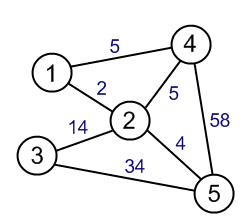
\includegraphics[scale=1]{Gambar/weight_graph}
\caption[Contoh Graf Berbobot]{Contoh Graf Berbobot}
\label{fig:weight_graph}
\end{figure}
Berdasarkan contoh pada Gambar \ref{fig:weight_graph}  didapatkan informasi tipe
dari node adalah bilangan bulat dan tipe dari bobot adalah bilangan bulat. \\
Himpunan node = {1,2,3,4,5} \\ 
Himpunan edge = {(1,4,5) ,(4,5,58) ,(3,5,34) ,(2,4,5) ,(2,5,4) ,(3,2,14) ,(1,2,2)} 

\subsection{Representasi Graf}
Terdapat dua cara untuk merepresentasikan graf yaitu dengan \textit{adjacency
list} dan \textit{adjacency matrix} \cite{Cormen:2001}. Keduanya dapat
merepresentasikan graf berarah ataupun graf tidak berarah. \textit{Adjacency list} merepresentasikan
graf ke dalam bentuk array, sedangkan \textit{adjacency matrix}
merepresentasikan graf ke dalam bentuk matriks.
\begin{itemize}
  \item \textit{Adjacency List}\\
  \textit{Adjacency List} merupakan representasi graf ke dalam bentuk array,
  panjang array sesuai dengan jumlah node pada graf. Setiap index pada array
  mengacu pada setiap node graf, setiap index array tersebut memiliki list yang
  merepresentasikan hubungan dengan node-node lainnya. Contoh representasi graf
  tidak berarah dalam bentuk \textit{adjacency list} dapat dilihat pada Gambar 
  \ref{fig:adjlist_undirec} dan representasi graf berarah
  dalam bentuk \textit{adjacency list} dapat dilihat pada Gambar
  \ref{fig:adjlist_direc}.
  
\begin{figure}[h]
\centering
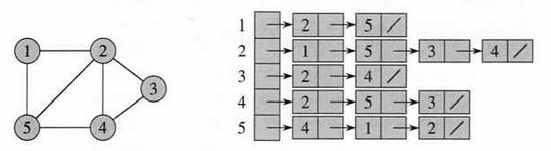
\includegraphics[scale=1]{Gambar/adjlist_undirec}
\caption[Contoh Adjacency List]{Contoh Adjacency List (Graf Tidak Berarah)}
\label{fig:adjlist_undirec}
\end{figure}

\begin{figure}[h]
\centering
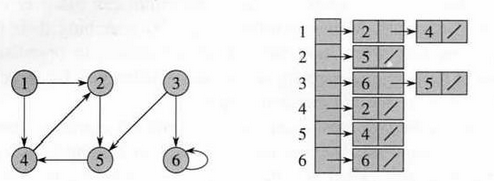
\includegraphics[scale=1]{Gambar/adjlist_direc}
\caption[Contoh Adjacency List]{Contoh Adjacency List (Graf Berarah)}
\label{fig:adjlist_direc}
\end{figure}
  
  \item \textit{Adjacency Matrix}\\
  \textit{Adjacency Matrix} merupakan representasi graf ke dalam bentuk matriks
  nxn, pada matriks tersebut menyatakan hubungan antar node atau pada graf.
  Nilai n pada matriks nxn sesuai dengan jumlah node pada graf. Nilai 1 pada
  matriks menandakan terdapat hubungan pada node dan sebaliknya jika bernilai
  0. Contoh representasi graf tidak berarah dalam bentuk \textit{adjacency
  matrix} dapat dilihat pada Gambar \ref{fig:adjmat_undirec} dan representasi
  graf berarah dalam bentuk \textit{adjacency matrix} dapat dilihat pada Gambar
  \ref{fig:adjmat_direc}.
  
\begin{figure}[h]
\centering
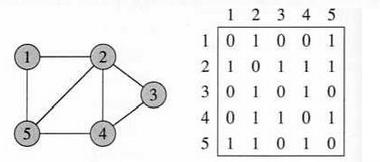
\includegraphics[scale=0.9]{Gambar/adjmat_undirec}
\caption[Contoh Adjacency Matrix]{Contoh Adjacency Matrix (Graf Tidak Berarah)}
\label{fig:adjmat_undirec}
\end{figure}

\begin{figure}[h]
\centering
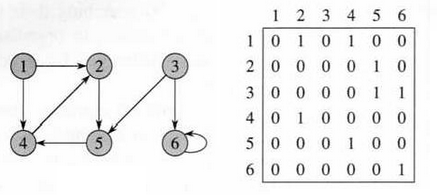
\includegraphics[scale=0.9]{Gambar/adjmat_direc}
\caption[Contoh Adjacency Matrix]{Contoh Adjacency Matrix (Graf Berarah)}
\label{fig:adjmat_direc}
\end{figure}
\end{itemize}

\section{Algoritma Dijkstra}
Algoritma dijkstra adalah algoritma yang dapat mencari jalur terpendek pada graf
berarah dengan persamaan G=(V,E) untuk kasus pada setiap sisinya bernilai tidak
negatif \cite{Cormen:2001}. Algoritma ini menggunakan prinsip greedy. Prinsip
greedy pada algoritma dijkstra adalah memilih sisi yang memiliki bobot paling
kecil dan memasukannya dalam himpunan solusi. Berikut ini adalah
\textit{pseudocode} dari algoritma dijkstra:
\begin{algorithm}{}\label{dijkstra}
\caption{$Dijkstra$}
\begin{algorithmic}
\State $dist[s] \leftarrow 0$
\ForAll{$v \in V$}
\State $dist[v] \leftarrow \infty$ 
\EndFor
\State $S \leftarrow \emptyset$
\State $Q \leftarrow V$
\While{$Q \neq \emptyset$} 
\State $u \leftarrow  minDistance(Q,dist)$
\State $S \leftarrow u$
\ForAll{$v \in neighbors[u]$}
\If{$dist[v] > dist[u] + w(u,  v)$}
\State $d[v] \leftarrow d[u] + w(u,  v)$
\EndIf
\EndFor
\EndWhile \\
\Return dist
\end{algorithmic}
\end{algorithm}

\section{Haversine \textit{Formula}}
Haversine \textit{formula} adalah persamaan yang dapat memberikan jarak antara
dua titik berdasarkan \textit{latitude} atau garis lintang dan
\textit{longitude} atau garis bujur \cite{haversine}. Haversine
\textit{formula} dinyatakan dalam persamaan berikut ini:
\\
\[d=2r\sin^{-1}(\sqrt{\sin^2(\frac{\phi_2-\phi_1}{2})+\cos(\phi_1)\cos(\phi_2)\sin^2(\frac{\psi_2-\psi_1}{2})})\]
dimana:
\begin{itemize}
  \item d : jarak antara dua buah titik
  
  \item r : radius bumi (6371 km)
   
  \item $\phi_1, \phi_2$ : \textit{latitude} dari titik 1 and \textit{latitude}
  dari titik 2
  
  \item $\psi_1, \psi_2$ : \textit{longitude} dari titik 1 and
  \textit{longitude} dari titik 2
\end{itemize}
}{}
\ifdefstring{\vbabc}{1}{\chapter{Analisis}
Pada bab ini akan dipaparkan analisis yang dilakukan dalam pembuatan aplikasi
ini. Bagaimana data XML didapatkan dari situs
\url{www.openstreetmap.org}, dibahas pada subbab \ref{ssec:analisis_osm}.
Pembacaannya menggunakan beberapa fungsi javascript, dibahas pada
subbab \ref{ssec:analisis_js}. Setelah itu, data tersebut disimpan atau dikonversi 
ke dalam bentuk graf sehingga dapat diimplementasikan algoritma
Dijkstra untuk mencari rute terpendek dari satu node ke node lain. Berdasarkan 
informasi yang telah diolah, maka dapat dibuat visualisasi data atau informasi
menggunakan Google Maps Javascript API. Pada akhir bab ini, juga dibahas
mengenai diagram \textit{use case} dan skenario untuk memperjelas apa saja 
yang dapat dilakukan oleh \textit{user} pada aplikasi ini.

\section{Analisis OpenStreetMap} \label{ssec:analisis_osm}
OpenStreetMap adalah portal peta terbuka yang menyediakan data dalam bentuk peta
ataupun dokumen XML. Aplikasi yang dibuat berbasis OpenStreetMap, hal ini
berarti aplikasi yang dibuat menggunakan data yang diperoleh dari situs
\url{www.openstreetmap.org}. Untuk mendapatkan data peta pada situs
OpenStreetMap, user harus mengunjungi situs tersebut dan menggunakan fitur
\textit{export}. Data yang digunakan adalah data peta yang berbentuk
dokumen XML atau biasa disebut dengan OSMXML. Selanjutnya, informasi yang
terkandung di dalam dokumen OSMXML tersebut diproses untuk mengetahui node dan
edge pada peta. Informasi tersebut akan diubah ke dalam bentuk graf yang akan
diproses lebih lanjut menggunakan algoritma Dijkstra untuk mengetahui jarak
terpendek dari satu node ke node lain.

\subsection{Langkah-Langkah Pengambilan Data OSMXML}
Berikut ini adalah langkah-langkah pengambilan data OSMXML yang akan digunakan:
\begin{enumerate}
  \item Mengunjungi situs \url{www.openstreetmap.org}.
  
  \item Menggunakan fitur \textit{search} untuk mencari area lokasi yang
  diinginkan. penggunaan fitur ini dapat dilihat pada Gambar
  \ref{fig:osmsearch_analisis} .
\begin{figure}[h]
\centering
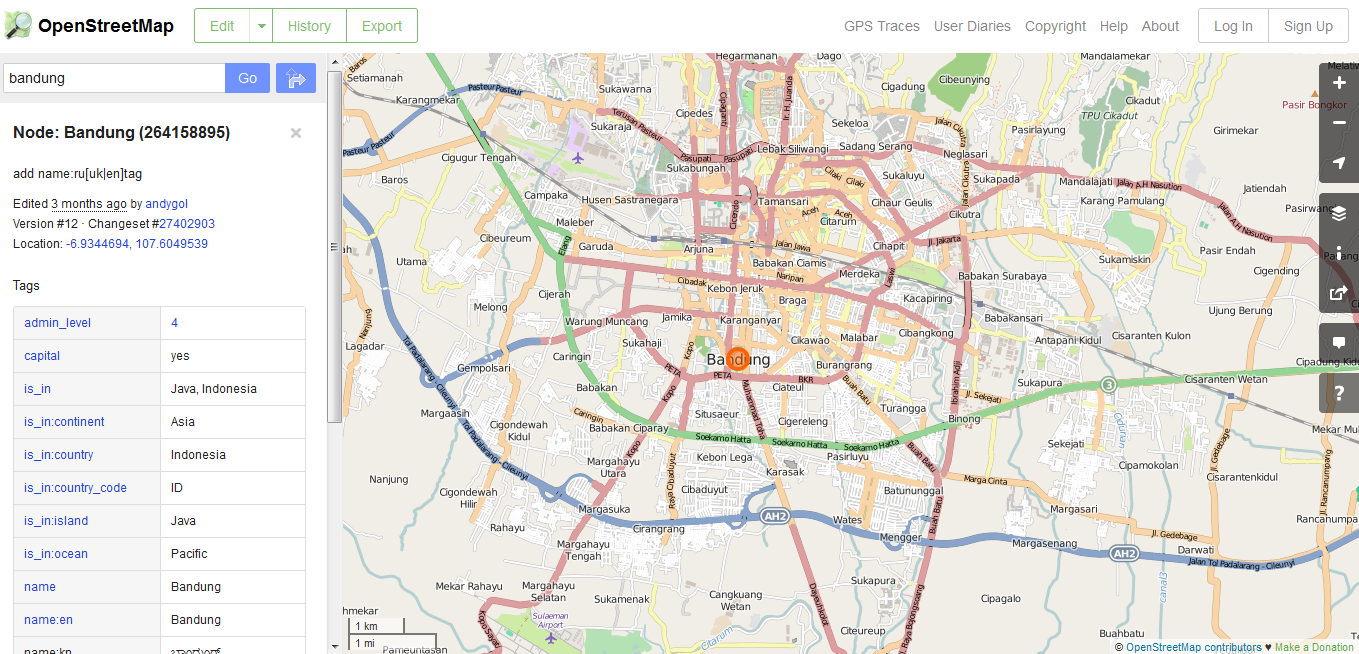
\includegraphics[scale=0.4]{Gambar/osmsearch_analisis}
\caption[Fitur search pada situs OpenStreetMap]{Fitur search pada situs
OpenStreetMap}
\label{fig:osmsearch_analisis}
\end{figure}
  
  \item Menggunakan fitur \textit{export} untuk mengunduh data dalam
  bentuk dokumen OSMXML. penggunaan fitur ini dapat dilihat pada Gambar
  \ref{fig:osmxml_analisis}.
\begin{figure}[h]
\centering
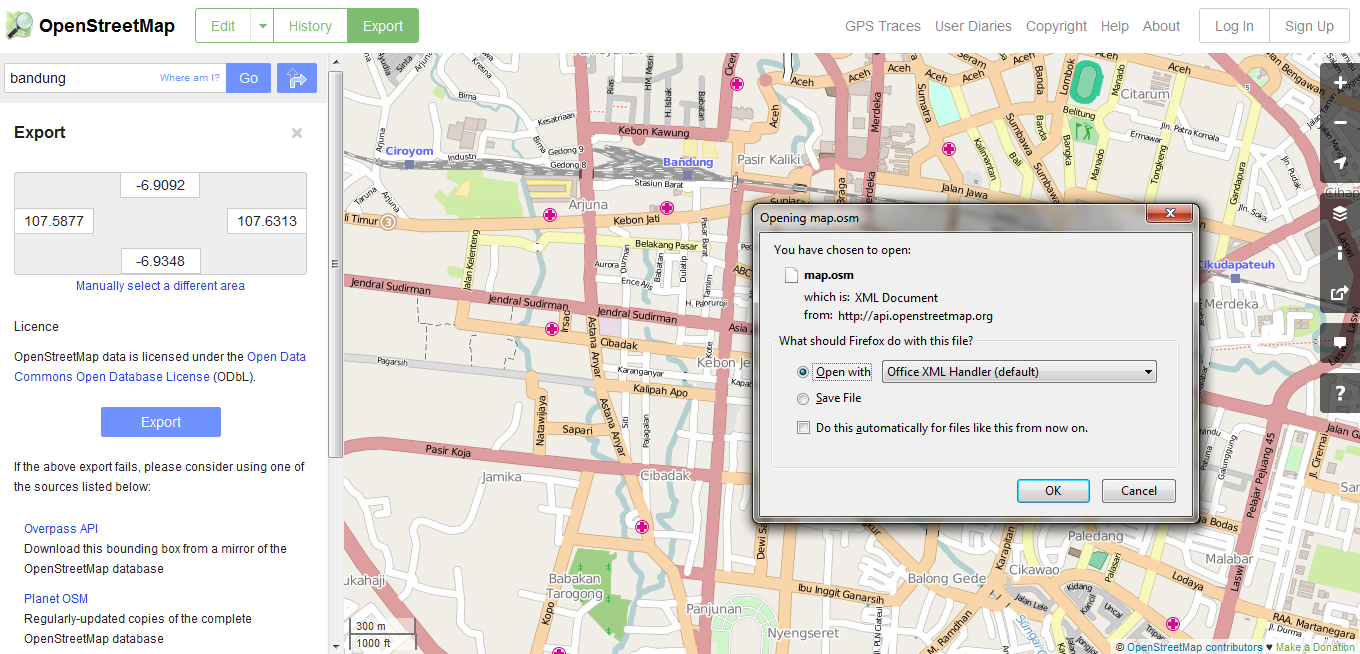
\includegraphics[scale=0.4]{Gambar/osmxml_analisis}
\caption[Fitur search pada situs OpenStreetMap]{Fitur \textit{export} pada situs
OpenStreetMap}
\label{fig:osmxml_analisis}
\end{figure}
\end{enumerate}

\subsection{OSMXML}
Sesuai dengan pembahasan pada subbab \ref{ssec:osmxml}, OSMXML merupakan dokumen
XML yang mengandung data-data peta OpenStreetMap. Berikut ini adalah dokumen
OSMXML yang sudah diunduh dan digunakan pada proses analisis.
\begin{lstlisting}
<?xml version="1.0" encoding="UTF-8"?>
<osm version="0.6" generator="CGImap 0.3.3 (29805 thorn-03.openstreetmap.org)" copyright="OpenStreetMap and contributors" attribution="http://www.openstreetmap.org/copyright" license="http://opendatacommons.org/licenses/odbl/1-0/">
 <bounds minlat="-6.9076500" minlon="107.5961800" maxlat="-6.9044500" maxlon="107.6016300"/>
 <node id="25418868" visible="true" version="6" changeset="27915808" timestamp="2015-01-04T17:54:58Z" user="isonpurba" uid="2552445" lat="-6.9064389" lon="107.5976351"/>
 <node id="25433683" visible="true" version="3" changeset="839915" timestamp="2009-03-21T14:18:48Z" user="adhitya" uid="7748" lat="-6.9067659" lon="107.5989458"/>
 ...
 <node id="25433687" visible="true" version="2" changeset="839915" timestamp="2009-03-21T14:18:36Z" user="adhitya" uid="7748" lat="-6.9040267" lon="107.5969508"/>
 <node id="25433688" visible="true" version="2" changeset="839915" timestamp="2009-03-21T14:18:58Z" user="adhitya" uid="7748" lat="-6.9039393" lon="107.5963723"/>
 <node id="25500626" visible="true" version="3" changeset="839915" timestamp="2009-03-21T14:22:17Z" user="adhitya" uid="7748" lat="-6.9070329" lon="107.6019401"/>
 ...
<node id="3030289971" visible="true" version="1" changeset="24892866" timestamp="2014-08-20T18:40:31Z" user="albahrimaraxsa" uid="2162153" lat="-6.9066710" lon="107.5982569"/>
 <node id="2325451442" visible="true" version="4" changeset="27916144" timestamp="2015-01-04T18:06:33Z" user="isonpurba" uid="2552445" lat="-6.9045011" lon="107.6024922"/>
 <way id="4567626" visible="true" version="4" changeset="15861148" timestamp="2013-04-25T13:56:12Z" user="mrdoggie94" uid="1331966">
  <nd ref="25433682"/>
  <nd ref="25433681"/>
  <nd ref="25433680"/>
  <tag k="avgspeed" v="15"/>
  <tag k="highway" v="residential"/>
  <tag k="name" v="Dr. Rubini"/>
 </way>
 <way id="4567634" visible="true" version="2" changeset="7821743" timestamp="2011-04-10T11:15:30Z" user="evo2mind" uid="234610">
  <nd ref="25433681"/>
  <nd ref="28802396"/>
  <tag k="avgspeed" v="15"/>
  <tag k="highway" v="residential"/>
  <tag k="name" v="Dr. Susilo"/>
 </way>
 ...
</osm>
\end{lstlisting}
Node dan way memiliki informasi penting yang digunakan pada aplikasi. Pada
tag node terdapat atribut id yang menunjukkan id pada setiap node, kemudian
terdapat atribut lat dan lon yang memberikan informasi titik koordinat
(\textit{latitude} dan \textit{longitude}) node tersebut. Informasi yang
didapatkan, disimpan ke dalam bentuk node pada graf. Tag way akan
menunjukkan hubungan pada node-node yang terdapat pada dokumen, dan disimpan
sebagai edge pada graf. Selain itu, tag way tidak hanya memberikan informasi 
jalan raya atau jalan besar saja, tetapi juga beberapa elemen peta
lain seperti area sekeliling bangunan atau area sekitar tempat parkir. Maka dari
itu, diperlukan \textit{filter} pada tag way, karena hanya informasi jalan raya
atau jalan besar saja yang diperlukan oleh aplikasi. Data atau dokumen OSMXML
yang telah diperoleh, selanjutnya dibaca menggunakan javascript yang dibahas
pada subbab \ref{ssec:analisis_js}.

\section{Analisis Javascript} \label{ssec:analisis_js}
Javascript diperlukan untuk membaca dokumen OSMXML, sehingga seluruh informasi
yang diperlukan dapat diubah ke dalam bentuk graf yang dapat diproses lebih
lanjut. XMLHttpRequest adalah salah satu objek pada javascript yang dapat
digunakan untuk mendapatkan \textit{file} XML. Berikut ini adalah langkah-langkah yang
dilakukan untuk membaca dokumen OSMXML menggunakan javascript:
\begin{enumerate}
  \item Membuat Objek XMLHttpRequest. 
\begin{verbatim}
xmlhttp=new XMLHttpRequest();
xmlhttp.open("GET","map.xml",false);
xmlhttp.send();
xmlDoc=xmlhttp.responseXML;
\end{verbatim}
Objek XMLHttpRequest digunakan untuk membaca \textit{file} XML yang telah
diunduh sebelumnya. Tahap-tahap yang dilakukan adalah sebagai berikut:
\begin{enumerate}
  \item Membuat objek XMLHttpRequest.
  
  \item Objek ini akan menginisialisasi permintaan dengan memanggil fungsi
  open(), pada kode program di atas menggunakan \textit{method} ``GET'' yaitu meminta dokumen ``map.xml'' 
  dan parameter ``false'' menunjukkan bahwa permintaan tersebut \textit{synchronous}.
  
  \item Objek mengirimkan permintaan yang telah diinisialisasi sebelumnya dengan
  memanggil \textit{method} send();
  
  \item Tahap terakhir adalah mendapatkan respon dari permintaan yang telah
  dikirimkan. Objek mengakses atribut responseXML, jika permintaan berhasil
  maka variabel xmlDoc akan berisi dokumen XML yang diminta, jika gagal maka
  variabel akan bernilai \textit{null}.
\end{enumerate}

  \item Menampilkan informasi node yang didapat pada layar.
\begin{verbatim}
document.write("<div style='float: left'>");
document.write("<table><tr><th>Node</th><th>Id</th>
<th>Latitude</th><th>Longitude</th></tr>");
document.write("<caption>Node</caption>");

var node=xmlDoc.getElementsByTagName("node");
for (i=0;i<node.length;i++){
  document.write("<tr><td>");
  document.write(i);
  document.write("</td><td>");
  document.write(node[i].getAttribute('id'));
  document.write("</td><td>");
  document.write(node[i].getAttribute('lat'));
  document.write("</td><td>");
  document.write(node[i].getAttribute('lon'));
  document.write("</td></tr>");
}
document.write("</table>");
document.write("</div>");
\end{verbatim}
Kode diatas menampilkan informasi node pada dokumen OSMXML dalam bentuk tabel.
Berikut ini adalah tahap-tahap yang dilakukan:
\begin{enumerate}
  \item Membuat tag <div> sebagai tempat tabel.
  
  \item Membuat tabel.
  
  \item Membuat variabel node, variabel ini berisi informasi seluruh node yang
  terdapat pada variabel xmlDoc, \textit{method} yang digunakan adalah
  getElementsByTagName(). Sebelumnya xmlDoc sudah berisi dengan dokumen ``map.xml''.
  
  \item Melakukan \textit{print} pada tabel, beberapa atribut yang ditampilkan
  adalah id node, \textit{latitude}, dan \textit{longitude}.
\end{enumerate}

  \item Membuat fungsi untuk melakukan \textit{filter} pada elemen way.
\begin{verbatim}
function isHighway(way,index){
  var tag = way[index].getElementsByTagName("tag");
  for (hg=0;hg<tag.length;hg++){
    if(tag[hg].getAttribute('k') == "highway"){
      return true;
    }
  }
  return false;
}
\end{verbatim}
\textit{Filter} dilakukan karena hanya elemen way yang berjenis \textit{highway}
saja yang akan digunakan. Berikut ini adalah tahap-tahap yang dilakukan:
\begin{enumerate}
  \item Membuat fungsi isHighway() dengan parameter \textit{input} way dan
  index. Parameter way berisi informasi seluruh way, sedangkan parameter index
  menunjukkan tag way pada index tersebut yang akan dicari.
  
  \item Membuat variabel yang menyimpan informasi way pada index yang dicari,
  pada kode program variabel tersebut diberi nama ``tag''.
  
  \item Lakukan pengulangan untuk mencari setiap \textit{child} pada variabel
  ``tag'' yang memiliki atribut ``k=highway'', jika ditemukan fungsi akan
  mengembalikan \textit{true} dan \textit{false} jika tidak ditemukan.
\end{enumerate}
	
	\item Menampilkan informasi way yang didapat pada layar.
\begin{verbatim}
document.write("<div style='margin-left: 20px;float: left'>");
document.write("<table><tr><th>Way</th><th>Id Way</th>
<th>Edge</th><th>Id Node 1</th><th>Id Node 2</th></tr>");
document.write("<caption>Edge</caption>");

var way = xmlDoc.getElementsByTagName("way");
var nd;
for (i=0;i<way.length;i++){
  nd = way[i].getElementsByTagName("nd");
  if(isHighway(way,i)){
    for (j=0;j<nd.length-1;j++){
      document.write("<tr><td>");
      document.write(i);
      document.write("</td><td>");
      document.write(way[i].getAttribute('id'));
      document.write("</td><td>");
      document.write(j);
      document.write("</td><td>");
      document.write(nd[j].getAttribute('ref'));
      document.write("</td><td>");
      document.write(nd[j+1].getAttribute('ref'));	
      document.write("</td></tr>");
    }
  }
}
document.write("</div>");
\end{verbatim}
Kode diatas menampilkan informasi way pada dokumen OSMXML dalam bentuk tabel.
\begin{enumerate}
  \item Membuat tag <div> sebagai tempat tabel.
  
  \item Membuat tabel.
  
  \item Membuat variabel way, variabel ini berisi informasi seluruh way yang
  terdapat pada variabel xmlDoc, \textit{method} yang digunakan adalah
  getElementsByTagName(). Sebelumnya xmlDoc sudah berisi dengan dokumen ``map.xml''.
  
  \item Membuat variabel yang berisi informasi way pada index tertentu, dan
  lakukan \textit{filter} dengan menggunakan fungsi isHighway().
  
  \item Melakukan \textit{print} pada tabel, beberapa atribut yang ditampilkan
  adalah id way, id node pertama, dan id node kedua.
\end{enumerate}
\end{enumerate}
\begin{figure}[h]
\centering
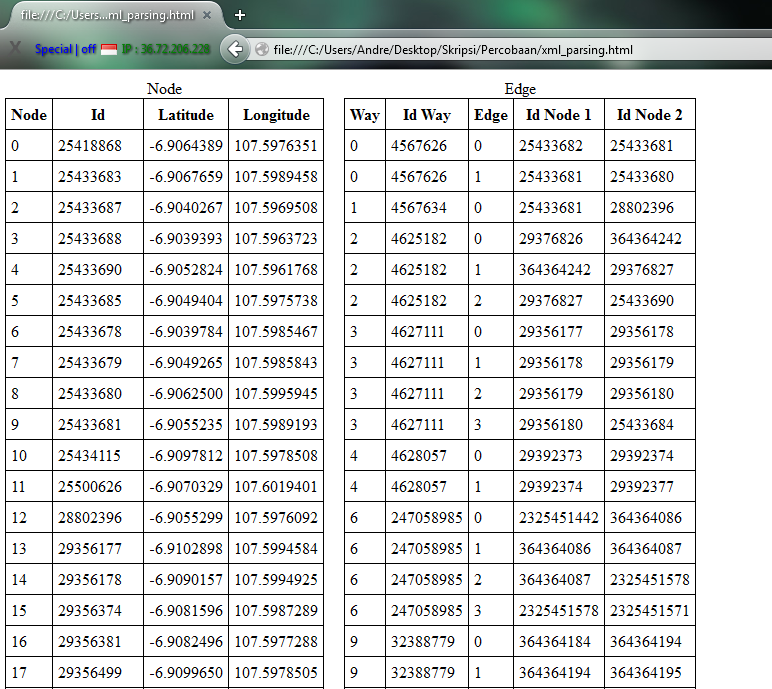
\includegraphics[scale=0.5]{Gambar/xml_parsing}
\caption[Parsing XML menggunakan Javascript]{Parsing XML menggunakan
Javascript}
\label{fig:xml_parsing}
\end{figure}
Hasil dari kode program di atas dapat dilihat pada Gambar \ref{fig:xml_parsing}.
Pada Gambar \ref{fig:xml_parsing} dapat dilihat terdiri dari dua tabel yang menunjukkan 
informasi node dan edge yang sudah dibaca. Tabel 
node menunjukkan atribut penting yang akan digunakan yaitu id node, \textit{latitude}, dan
\textit{longitude}. Sedangkan tabel edge menujukkan informasi yang didapatkan
dari tag way yang sudah dilakukan \textit{filter}, yaitu hanya tag way yang
memiliki \textit{child} highway saja yang akan digunakan. Pada tabel edge
terdapat informasi penting yang akan digunakan, yaitu id way, id node pertama, 
dan id node kedua. Informasi yang sudah didapatkan, selanjutnya akan dimodelkan
ke dalam bentuk graf yang akan dibahas pada subbab \ref{ssec:analisis_graf}.

\section{Menghitung Jarak Antara Dua Titik}
Untuk menghitung jarak antara dua titik dapat digunakan rumus haversine atau
dikenal dengan haversine \textit{formula}. Analisis rumus haversine dilakukan
dengan implementasi rumus tersebut dengan contoh kasus perhitungan
jarak antara koordinat Kota Bandung (-6.9167,107.6000) dan koordinat Kota
Jakarta (-6.1745,106.8227). Berikut ini adalah rumus haversine yang telah
diimplementasikan:
\begin{verbatim}
function getDistance(lat1,lon1,lat2,lon2){
  var R = 6371; 
  var dLat = deg2rad(lat2-lat1); 
  var dLon = deg2rad(lon2-lon1); 
  var a = 
    Math.sin(dLat/2) * Math.sin(dLat/2) +
    Math.cos(deg2rad(lat1)) * Math.cos(deg2rad(lat2)) * 
    Math.sin(dLon/2) * Math.sin(dLon/2); 
  var c = 2 * Math.atan2(Math.sqrt(a), Math.sqrt(1-a)); 
  var d = R * c; 
  return d;
}

function deg2rad(deg){
  return deg * (Math.PI/180);
}
\end{verbatim}
Hasil yang ditunjukkan dari rumus haversine adalah 119.09781542340916 km dapat
dilihat pada Gambar \ref{fig:analisis_haver}.

\begin{figure}[h]
\centering
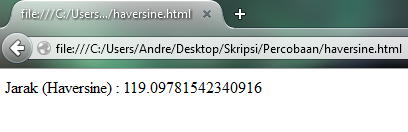
\includegraphics[scale=1]{Gambar/analisis_haver}
\caption[Perhitungan Jarak Dengan Haversine Formula]{Perhitungan Jarak Dengan Haversine Formula}
\label{fig:analisis_haver}
\end{figure}
Saat proses analisis, ternyata Google Maps Javascript API menyediakan suatu
\textit{library} untuk mengukur jarak antara dua titik. \textit{Library}
tersebut adalah \textit{geometry library} yang menyediakan fungsi utilitas yaitu
google.maps.geometry.spherical. Google tidak mempublikasikan algoritma yang
digunakan untuk perhitungan jarak tersebut. Untuk menghitung jarak antara dua titik
digunakan fungsi computeDistanceBetween(). Sama seperti rumus haversine,
analisis fungsi computeDistanceBetween() dilakukan dengan implementasi contoh
kasus perhitungan jarak antara koordinat Kota Bandung dan Jakarta. Berikut ini
adalah fungsi computeDistanceBetween() yang telah diimplementasikan:
\begin{verbatim}
var jakarta = new google.maps.LatLng(-6.1745,106.8227);
var bandung = new google.maps.LatLng(-6.9167,107.6000);
var distance = google.maps.geometry.spherical.
computeDistanceBetween(jakarta, bandung);
\end{verbatim}
Hasil yang ditunjukkan dari fungsi computeDistanceBetween() adalah
119.23123264342443 km dapat dilihat pada Gambar \ref{fig:analisis_geometry}.

\begin{figure}[h]
\centering
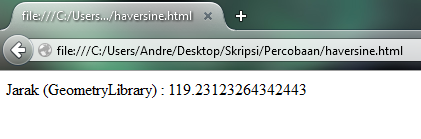
\includegraphics[scale=1]{Gambar/analisis_geometry}
\caption[Perhitungan Jarak Dengan Geometry Library]{Perhitungan Jarak Dengan
Geometry Library}
\label{fig:analisis_geometry}
\end{figure}
Terdapat perbedaan atau selisih yang dihasilkan oleh rumus haversine dan
fungsi computeDistanceBetween() sebesar 0.133417220015275 km. Fungsi 
computeDistanceBetween() yang akan digunakan untuk pembuatan aplikasi, bukan
rumus haversine. Hal ini karena aplikasi menggunakan Google Maps Javascript
API, sehingga fungsi tersebut lebih cocok untuk digunakan.

\section{Pemodelan OSMXML Menjadi Graf} \label{ssec:analisis_graf}
Pada subbab \ref{ssec:analisis_js}, dokumen OSMXML sudah dibaca dan tahap
selanjutnya adalah memodelkan data OSMXML tersebut ke dalam bentuk graf. Seperti
yang sudah diketahui, graf terdiri dari node dan edge. Informasi node dan edge
yang sudah didapatkan akan dimodelkan ke dalam bentuk graf berarah, hal ini
karena jalan yang menghubungkan node-node tersebut memiliki arah, baik searah
maupun dua arah, arah jalan diketahui dengan melihat informasi tag oneway. Untuk
merepresentasikan graf tersebut, digunakan \textit{adjacency list}.
Penggunaan \textit{adjacency list} disebabkan oleh penggunaan memori yang lebih
kecil dibandingkan dengan \textit{adjacency matrix}. Hal ini karena, setelah
dilakukan \textit{filter} diketahui bahwa graf tersebut berjenis
\textit{sparse} (graf yang memiliki jumlah edge dekat dengan jumlah minimum
edge). Berikut ini adalah langkah-langkah yang dilakukan untuk memodelkan OSMXML
menjadi graf:
\begin{enumerate}
  \item Membuat kelas Node dan kelas Neighbor.
\begin{verbatim}
function Node(id, neighbors){
  this.id = id;
  this.adjList = neighbors;
}

function Neighbor(vnum, nbr, weight){
  this.vertexNum = vnum;
  this.weight = weight;
  this.next = nbr;
}
\end{verbatim}
Kedua kelas tersebut digunakan untuk menyimpan informasi id node dan jarak. Id
node disimpan pada kelas node menggunakan atribut id, sedangkan jarak disimpan
pada kelas neighbor menggunakan atribut weight.

  \item Membaca seluruh informasi node dan menyimpan pada kelas node.
\begin{verbatim}
var adjLists = [];
for(i=0;i<node.length;i++){
  adjLists.push(new Node(node[i].getAttribute('id'),null));
}
\end{verbatim}
  Berikut ini adalah tahap-tahap yang dilakukan untuk menyimpan seluruh
  informasi tersebut:
  \begin{enumerate}
    \item Membuat variabel adjLists, variabel ini bertipe array.
    
    \item Lakukan pengulangan untuk memasukkan informasi node satu persatu.
  \end{enumerate}

  \item Membuat fungsi untuk menentukan arah pada setiap node yang terhubung
  dengan node lain.
\begin{verbatim}
function wayDirection(way,index){
  var tag = way[index].getElementsByTagName("tag");
  for (hg=0;hg<tag.length;hg++){
    if(tag[hg].getAttribute('k') == "oneway"){
      return tag[hg].getAttribute('v');
    }
  }
  return false;
}
\end{verbatim}
  Berikut ini adalah tahap-tahap yang dilakukan:
  \begin{enumerate}
  \item Membuat fungsi wayDirection() dengan parameter \textit{input} way dan
  index. Parameter way berisi informasi seluruh way, sedangkan parameter index
  menunjukkan tag way pada index tersebut yang akan dicari informasi arahnya.
  
  \item Membuat variabel yang menyimpan informasi way pada index yang dicari,
  pada kode program variabel tersebut diberi nama ``tag''.
  
  \item Lakukan pengulangan untuk mencari setiap \textit{child} pada variabel
  ``tag'' untuk mencari atribut ``k=oneway'', jika ditemukan fungsi akan
  mengembalikan \textit{value} dari \textit{key} tersebut dan \textit{false}
  jika tidak ditemukan.
  \end{enumerate}

  \item Membuat fungsi untuk mendapatkan informasi koordinat node
  (\textit{latitude} dan \textit{longitude}).
\begin{verbatim}
function getLatByAtt(str){
  for (n=0;n<node.length;n++){
    if(node[n].getAttribute('id') == str){
      return node[n].getAttribute('lat');
    }
  }
  return -1;
}

function getLonByAtt(str){
  for (m=0;m<node.length;m++){
    if(node[m].getAttribute('id') == str){
      return node[m].getAttribute('lon');
    }
  }
  return -1;
}
\end{verbatim}
  Kode di atas terdiri dari dua fungsi, fungsi getLatByAtt() mencari informasi
  \textit{latitude} dan fungsi getLatByAtt() mencari informasi
  \textit{longitude}. Kedua fungsi tersebut melakukan pencarian node berdasarkan
  parameter \textit{input} str yang merupakan id node, jika ditemukan fungsi
  akan mengembalikan nilai \textit{latitude} atau \textit{longitude} dan
  mengembalikan nilai -1 jika tidak ditemukan.

  \item Membaca seluruh informasi edge yang terdapat pada tag way. Berikut ini
  adalah tahap-tahap yang dilakukan:
  \begin{enumerate}
    \item Melakukan pengulangan untuk setiap way.
    
    \item Melakukan \textit{filter} untuk setiap way, hanya ``highway'' saja
    yang akan dimasukkan informasinya ke dalam \textit{adjacency list}.
    
    \item Melakukan pemanggilan fungsi wayDirection() dan memasukkan nilai
    didapatkan dari fungsi tersebut ke variabel, pada kode di atas menggunakan
    variabel ``oneway''.
    
    \item Cari jarak antar node.
    
    \item Memasukkan informasi edge berdasarkan arah yang dimasukkan ke dalam
    variabel ``oneway''.
  \end{enumerate}

  \item Membuat fungsi untuk menampilkan graf ke layar
\begin{verbatim}
function print(list){
  for (j=0; j < list.length; j++){
    document.write(j);
    for (nbr=list[j].adjList; nbr != null;nbr=nbr.next) {
      document.write("---->");
      document.write('('+nbr.vertexNum+')');
    }
    document.write("<br>");
  }
}
\end{verbatim}
  Fungsi akan menerima parameter \textit{input} berupa array, yaitu
  variabel adjLists. Selanjutnya dilakukan pembacaan setiap index array dan
  hasilnya ditampilkan di layar.
\end{enumerate}
Hasil dari kode program di atas dapat dilihat pada Gambar
\ref{fig:graf_analisis}.
Pada Gambar \ref{fig:graf_analisis}, data pada OSMXML sudah dimodelkan ke dalam
bentuk graf menggunakan representasi \textit{adjacency list}. Tahap
selanjutnya, graf tersebut akan divisualisasikan menggunakan Google Maps
Javascript API yang dibahas pada subbab \ref{ssec:analisis_gmap}.
\clearpage
\begin{figure}[h]
\centering
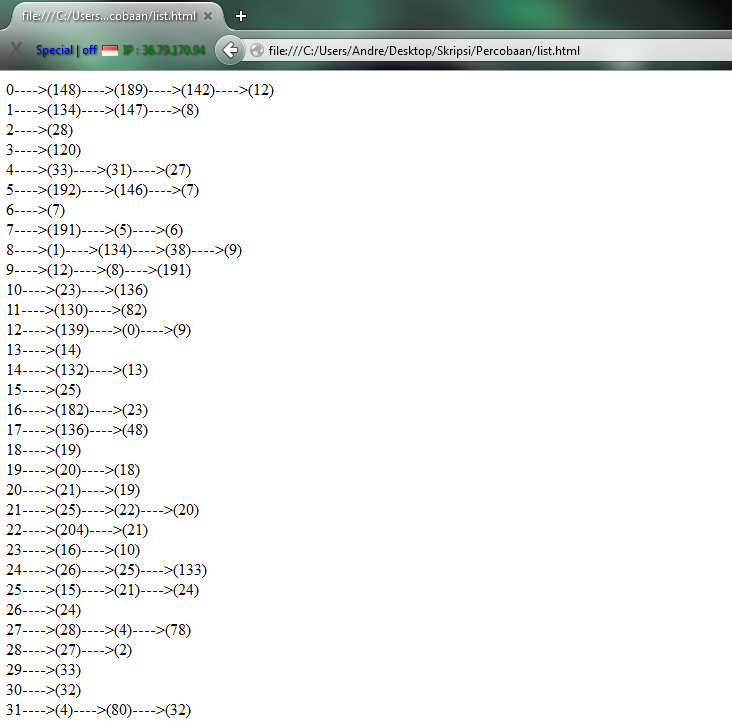
\includegraphics[scale=0.5]{Gambar/graf_analisis}
\caption[Pemodelan OSMXML menjadi Graf]{Pemodelan OSMXML menjadi Graf}
\label{fig:graf_analisis}
\end{figure}

\section{Visualisasi} \label{ssec:analisis_gmap}
Data OSMXML yang sudah dimodelkan ke dalam bentuk graf, selanjutnya
divisualisasikan menggunakan Google Maps Javascript API. Peta ditampilkan dalam 
bentuk \textit{roadmap}, karena peta jenis ini memberikan 
informasi mengenai nama jalan, sehingga peta jenis ini lebih cocok untuk aplikasi 
yang dibangun. Berikut ini langkah-langkah yang dilakukan untuk membuat
visualisasi graf:
\begin{enumerate}
  \item Melakukan \textit{load} Google Maps Javascript API.
\begin{verbatim}
<script src="https://maps.googleapis.com/maps/api
/js?v=3.exp&libraries=geometry"></script>
\end{verbatim}

  \item Membuat elemen div sebagai wadah atau tempat untuk peta.
\begin{verbatim}
<div id="googleMap" style="width:75%;height:600px;float:left"></div>
\end{verbatim}
  
  \item Membuat objek google.maps.Map dengan parameter \textit{input map
  options} (variabel mapProp). Peta disisipkan pada elemen div yang memiliki id
  googleMap.
\begin{verbatim}
var mapProp = {
  center:new google.maps.LatLng(-6.906845432118958,107.59851515293121),
  zoom:17,
  mapTypeId:google.maps.MapTypeId.ROADMAP
};

var map=new google.maps.Map(document.getElementById("googleMap"),mapProp);
\end{verbatim}
  Berikut ini tahap-tahap yang dilakukan:
  \begin{enumerate}
    \item Membuat variabel untuk mendefinisikan properti peta, pada kode
    di atas dilakukan pengaturan titik tengah, zoom pada level 17, dan tipe peta
    yaitu ``ROADMAP''.
    
    \item Membuat objek google.maps.Map, objek tersebut memiliki parameter
    properti peta (variabel mapProp), selanjutnya peta disisipkan pada elemen
    div yang memiliki id googleMap.
  \end{enumerate}

  \item Membuat objek \textit{marker} untuk setiap node pada peta.
\begin{verbatim}
for (j=0;j<nd.length;j++){
  id = uniqueId();
  marker = new google.maps.Marker({
    id: id,
    position: new google.maps.LatLng(getLatByAtt(nd[j].getAttribute('ref')),
    getLonByAtt(nd[j].getAttribute('ref'))), map: map,
    icon: image,
  });
  markers[id] = marker;
\end{verbatim}
  Dilakukan pengulangan untuk setiap node dan membuat objek \textit{marker},
  membaca atribut \textit{latitude} dan \textit{longitude}, lalu menampilkan
  seluruh \textit{marker} pada peta.

  \item Membuat objek \textit{polyline} yang menghubungkan setiap node pada
  peta.
\begin{verbatim}
for (k=0;k<nd.length-1;k++){
  line = new google.maps.Polyline({
    path: [new google.maps.LatLng(getLatByAtt(nd[k].getAttribute('ref')),
    getLonByAtt(nd[k].getAttribute('ref'))), new
    google.maps.LatLng(getLatByAtt(nd[k+1].getAttribute('ref')),
    getLonByAtt(nd[k+1].getAttribute('ref')))], 
    strokeColor: "#000000",
    strokeOpacity: 1.0, 
    strokeWeight: 3,
    map: map
  });
}
\end{verbatim}
  
  \item Membuat fungsi untuk menambahkan \textit{info window} pada setiap node
  untuk memberikan informasi id dan index node.
\begin{verbatim}
function addInfoWindow(marker, message) {
  var infoWindow = new google.maps.InfoWindow({
    content: message
  });
  
  google.maps.event.addDomListener(marker, 'click', function () {
    infoWindow.open(map, marker);
  });
}
\end{verbatim}
  Berikut ini adalah tahap-tahap yang dilakukan:
  \begin{enumerate}
    \item Membuat fungsi addInfoWindow dengan parameter \textit{input} yaitu
    \textit{marker} dan pesan.
    
    \item Membuat objek google.maps.InfoWindow.
    
    \item Menambahkan objek google.maps.InfoWindow pada \textit{listener} yang
    berasosiasi dengan parameter \textit{marker}.
  \end{enumerate}
\end{enumerate}
\begin{figure}[h]
\centering
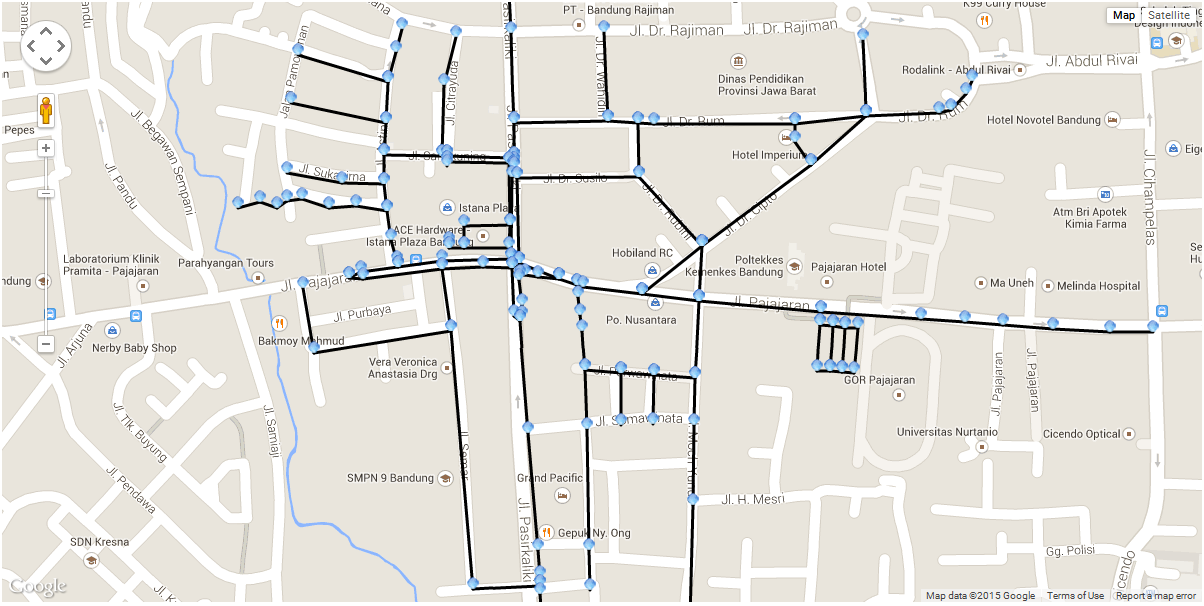
\includegraphics[scale=0.5]{Gambar/visualisasi_graf}
\caption[Visualisasi]{Visualisasi}
\label{fig:visualisasi}
\end{figure}
Hasil dari langkah-langkah di atas dapat dilihat pada Gambar
\ref{fig:visualisasi}. Setiap node pada graf yang sudah dilakukan
\textit{filter} akan diwakili oleh marker. Setiap marker tersebut akan memiliki \textit{info
window} yang akan memberikan informasi seperti id node, index node pada graf,
dan dua buah \textit{hyperlink} yang berfungsi untuk menjadikan marker yang
dipilih menjadi asal atau tujuan. Contoh \textit{info window} yang ditampilkan
pada peta dapat dilihat pada Gambar \ref{fig:visualisasi_infowindow}. Setiap
edge pada graf akan menjadi garis pada peta yang dibuat menggunakan \textit{polyline}.
\clearpage
\begin{figure}[h]
\centering
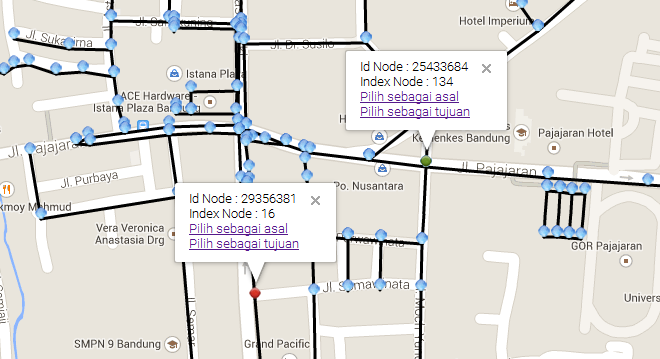
\includegraphics[scale=0.9]{Gambar/visualisasi_infowindow}
\caption[Info Window]{Info Window}
\label{fig:visualisasi_infowindow}
\end{figure}

\section{Algoritma Dijkstra}
Untuk pencarian rute terdekat, aplikasi menggunakan algoritma Dijkstra.
Algoritma tersebut diimplementasikan pada graf yang sudah dimodelkan
sebelumnya. Fungsi dijkstra menerima \textit{input} berupa objek ``edge''
yang berisi informasi dari graf, selanjutnya fungsi akan mengeluarkan \textit{output}
yaitu jalur terpendek dari satu titik ke titik lain dalam bentuk array. Untuk
hasil implementasi algoritma Dijkstra dapat dilihat pada Bab 5. Contoh kasus
yang digunakan, yaitu mencari rute terdekat dari titik asal ``16'' dan 
titik tujuan ``198'', output yang dihasilkan dapat dilihat pada Gambar
\ref{fig:output_dijkstra}.
\begin{figure}[h]
\centering
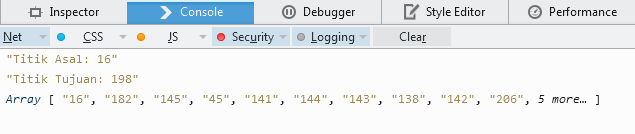
\includegraphics[scale=0.9]{Gambar/output_dijkstra}
\caption[Keluaran fungsi Dijkstra]{Keluaran fungsi Dijkstra}
\label{fig:output_dijkstra}
\end{figure}
Visualisasi rute terdekat dapat dilihat pada Gambar
\ref{fig:visualisasi_dijkstra}.
 \begin{figure}[h]
\centering
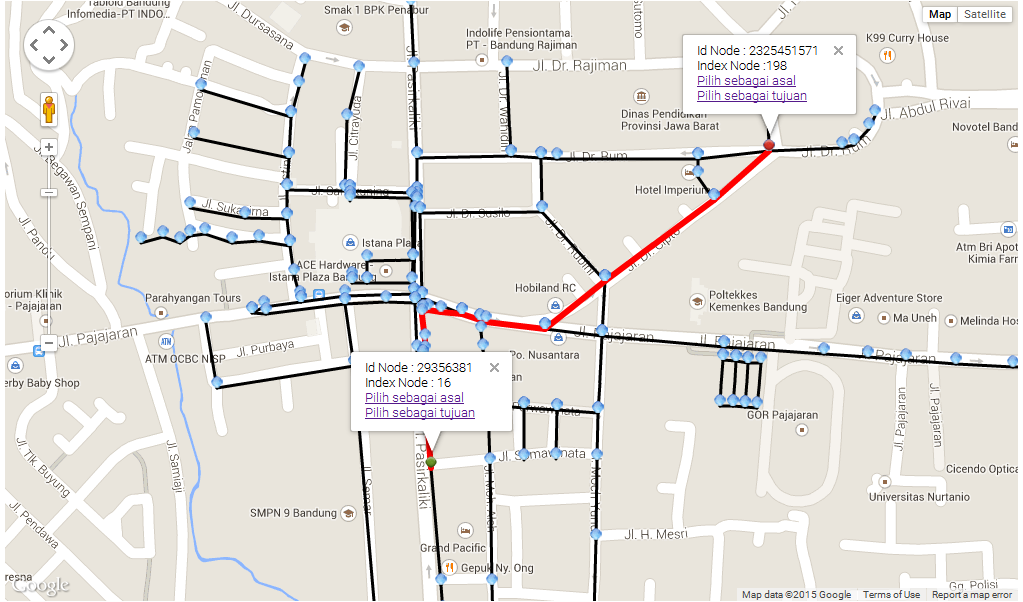
\includegraphics[scale=0.6]{Gambar/visualisasi_dijkstra}
\caption[Visualisasi Rute Terdekat]{Visualisasi Rute Terdekat}
\label{fig:visualisasi_dijkstra}
\end{figure}

\section{Analisis Berorientasi Objek}
Aplikasi pencarian rute terdekat yang dibangun akan mengolah data yang
disediakan oleh OpenStreetMap dalam bentuk XML dan memodelkannya ke dalam bentuk graf. 
\textit{User} dapat memilih titik asal dan titik tujuan, selanjutnya akan
diimplementasikan algoritma Dijkstra untuk mencari rute terdekat antara kedua titik 
tersebut dan menunjukkan hasilnya secara visual menggunakan Google Maps
Javascript API. Pada subbab ini akan membahas interaksi antara \textit{user}
dengan sistem yaitu menggunakan diagram \textit{use case} dan skenario. Setelahnya,
dibahas juga diagram kelas untuk menunjukkan kelas-kelas yang ada pada sistem
dan hubungannya.

\subsection{Diagram \textit{Use Case}}
Diagram \textit{use case} adalah pemodelan yang berfungsi memperjelas interaksi
antara aktor atau \textit{user} dengan sistem. 
Diagram \textit{use case} aplikasi pencarian rute terdekat dapat dilihat pada
Gambar \ref{fig:usecase}.
Berdasarkan analisis yang telah dilakukan, maka \textit{user} dapat melakukan
interaksi sebagai berikut:
\begin{enumerate}
  \item Memilih titik asal.\\
  \textit{User} dapat menekan salah satu \textit{marker} yang ada pada peta dan
  menekan \textit{link} ``pilih titik asal''. Selanjutnya, akan ditampilkan
  informasi titik yang sudah dipilih pada sisi kanan layar.
  
  \item Memilih titik tujuan.\\
  \textit{User} dapat menekan salah satu \textit{marker} yang ada pada peta dan
  menekan \textit{link} ``pilih titik tujuan''. Selanjutnya, akan ditampilkan
  informasi titik yang sudah dipilih pada sisi kanan layar.
  
  \item Mencari rute terdekat dari titik asal ke titik tujuan.\\
  \textit{User} dapat menekan tombol ``Cari'' untuk mencari rute terdekat dari
  kedua titik yang telah dipilih sebelumnya.
\end{enumerate}
\begin{figure}[h]
\centering
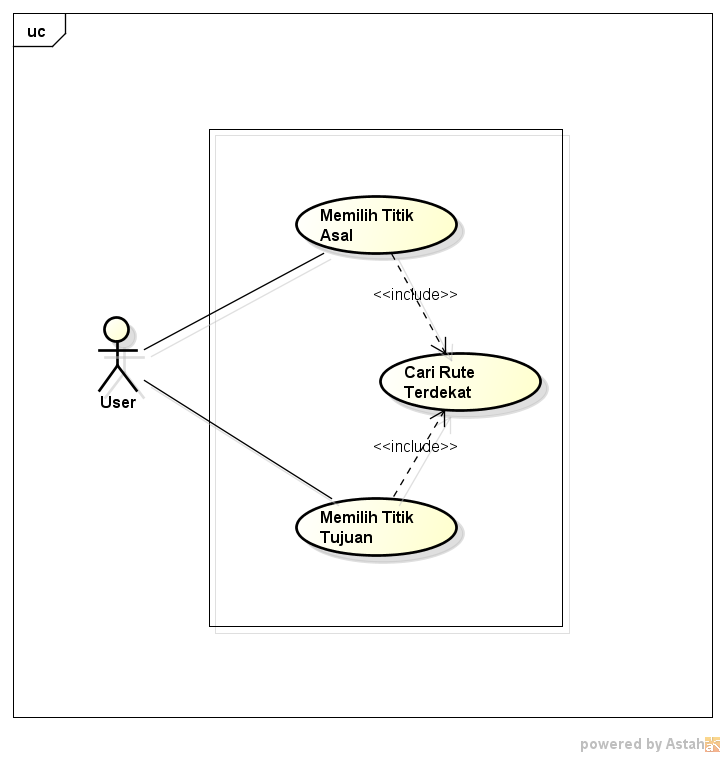
\includegraphics[scale=0.65]{Gambar/usecase}
\caption[Diagram Use Case]{Diagram \textit{use case}}
\label{fig:usecase}
\end{figure}

\subsection{Skenario}
Berikut ini adalah skenario untuk setiap \textit{use case}:
\begin{enumerate}
  \item Skenario memilih titik asal dapat dilihat pada Tabel
  \ref{tab:titik_asal}.  
\begin{table}[h]
\caption{Skenario memilih titik asal} 
\label{tab:titik_asal}
\begin{tabular}{|c|c|}
\hline
Nama          & Memilih titik asal                                              \\ \hline
Aktor         & User                                                            \\ \hline
Kondisi Awal  & Titik asal belum terpilih                                       \\ \hline
Kondisi Akhir & Titik asal sudah terpilih dan ditampilkan di sisi kanan layar   \\ \hline
Skenario      & User menekan marker pada peta dan menekan link pilih titik asal \\ \hline
Deskripsi     & User memilih titik pada peta untuk dijadikan titik asal         \\ \hline
Eksepsi       & -                                                               \\ \hline
\end{tabular}
\end{table}

  \item Skenario memilih titik tujuan dapat dilihat pada Tabel
  \ref{tab:titik_tujuan}.
\begin{table}[h]
\caption{Skenario memilih titik tujuan} 
\label{tab:titik_tujuan}
\begin{tabular}{|c|c|}
\hline
Nama          & Memilih titik tujuan                                              \\ \hline
Aktor         & User                                                              \\ \hline
Kondisi Awal  & Titik tujuan belum terpilih                                       \\ \hline
Kondisi Akhir & Titik tujuan sudah terpilih dan ditampilkan di sisi kanan layar   \\ \hline
Skenario      & User menekan marker pada peta dan menekan link pilih titik tujuan \\ \hline
Deskripsi     & User memilih titik pada peta untuk dijadikan titik tujuan         \\ \hline
Eksepsi       & -                                                                 \\ \hline
\end{tabular}
\end{table}

  \item Skenario cari rute terdekat dapat dilihat pada Tabel
  \ref{tab:rute_terdekat}.
\begin{table}[h]
\caption{Skenario cari rute terdekat} 
\label{tab:rute_terdekat}
\begin{tabular}{|c|c|}
\hline
Nama          & Cari rute terdekat                                                                                        \\ \hline
Aktor         & User                                                                                                      \\ \hline
Kondisi Awal  & Titik asal dan titik tujuan sudah terpilih                                                                \\ \hline
Kondisi Akhir & Sistem menampilkan rute terdekat menggunakan polyline                                                     \\ \hline
Skenario      & User menekan tombol Cari!                                                                                 \\ \hline
Deskripsi     & \begin{tabular}[c]{@{}c@{}}User menekan tombol Cari! dan sistem menampilkan rute \\ terdekat\end{tabular}                        \\ \hline
Eksepsi       & \begin{tabular}[c]{@{}c@{}}Jika user belum memilih titik asal atau tujuan \\ akan ditampilkan alert atau peringatan\end{tabular} \\ \hline
\end{tabular}
\end{table}
\end{enumerate}

\subsection{Diagram Kelas Sederhana}
Pada bagian ini, akan dijelaskan diagram kelas yang digunakan untuk memenuhi
kebutuhan \textit{user} yang sudah dijelaskan pada bagian diagram \textit{use
case} dan skenario. Berikut ini adalah diagram kelas sederhana yang dapat
dilihat pada Gambar \ref{fig:diagram_kelas}.
\begin{figure}[h]
\centering
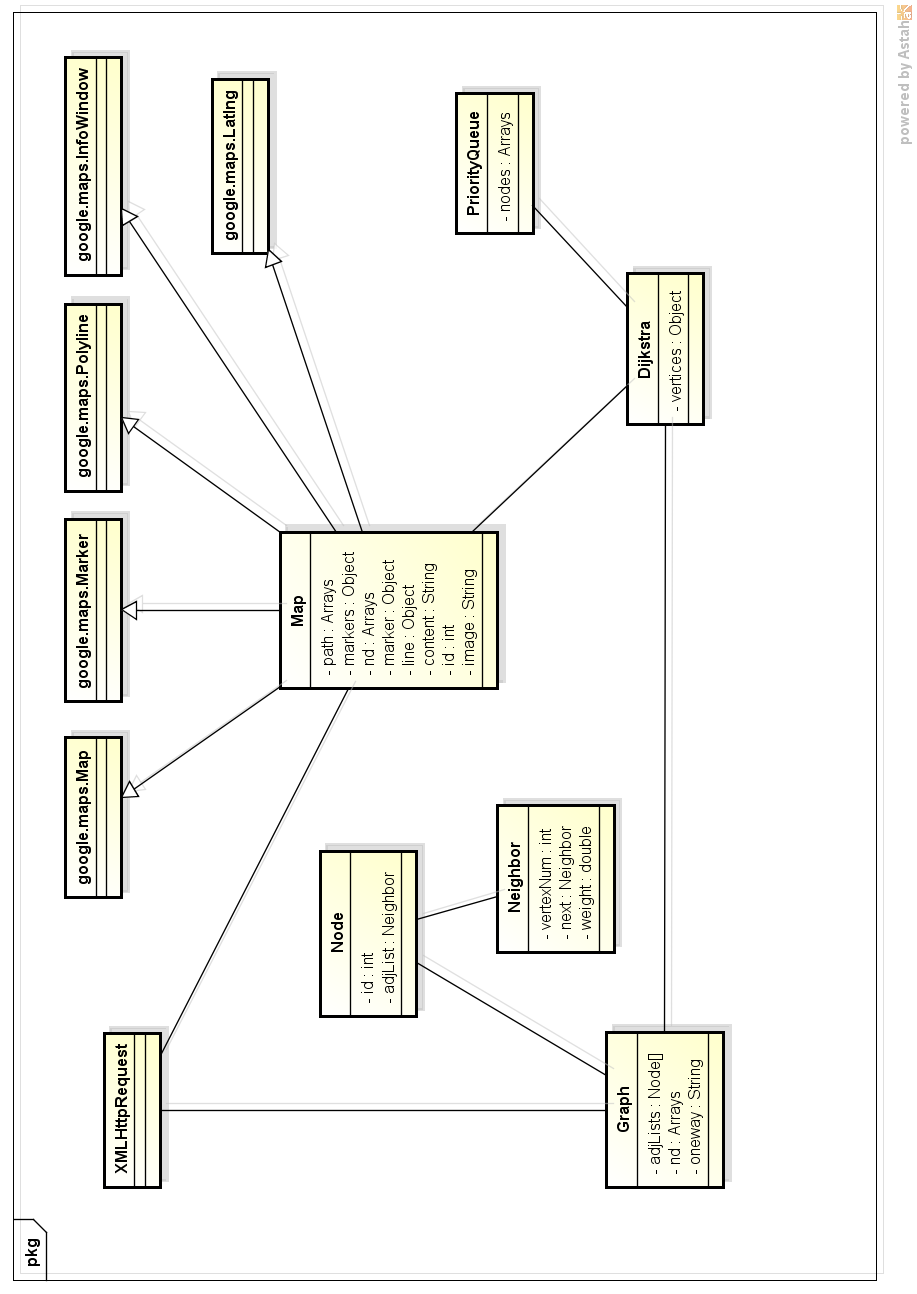
\includegraphics[scale=0.6]{Gambar/diagram_kelas}
\caption[Diagram Kelas Sederhana]{Diagram Kelas Sederhana}
\label{fig:diagram_kelas}
\end{figure}
Berikut ini adalah penjelasan dari setiap kelas yang terdapat pada diagram
kelas sederhana:
\begin{itemize}
  \item Kelas XMLHttpRequest\\
  Kelas ini berfungsi untuk melakukan \textit{load} dokumen OSMXML.
  
  \item Kelas Node dan Neighbor\\
  Kedua kelas ini akan menyimpan informasi yang didapatkan dari OSMXML sebagai
  representasi dari graf yaitu \textit{adjacency list}.
  
  \item Kelas Graph\\
  Kelas ini berfungsi untuk mengubah informasi yang didapatkan dari OSMXML
  menjadi graf.
  
  \item Kelas Map\\
  Kelas ini berfungsi untuk melakukan \textit{generate} peta, visualisasi graf,
  dan visualisasi rute terdekat.
  
  \item Kelas google.maps.Map\\
  Kelas ini berfungsi untuk membuat objek peta.
  
  \item Kelas google.maps.Marker\\
  Kelas ini berfungsi untuk membuat objek \textit{marker} yang akan digunakan
  sebagai visualisasi node pada peta.
  
  \item Kelas google.maps.Polyline\\
  Kelas ini berfungsi untuk membuat objek \textit{polyline} yang akan digunakan
  sebagai visualisasi edge pada peta.
  
  \item Kelas google.maps.InfoWindow\\
  Kelas ini berfungsi untuk membuat objek \textit{InfoWindow} yang akan
  disisipkan pada setiap objek \textit{marker}.
  
  \item Kelas google.maps.Latlng\\
  Kelas ini berfungsi untuk membuat objek Latlng. Latlng merupakan objek yang
  berisi informasi koordinat (\textit{latitude} dan \textit{longitude}).
  
  \item Kelas Dijkstra\\
  Kelas ini berfungsi untuk mencari rute terdekat berdasarkan \textit{input}
  titik asal dan titik tujuan.
  
  \item Kelas PriorityQueue\\
  Kelas ini merupakan struktur data \textit{queue} yang digunakan pada
  kelas dijkstra.
\end{itemize}



















}{}
\ifdefstring{\vbabd}{1}{\chapter{Perancangan}
Pada bab ini dijelaskan perancangan aplikasi pencarian rute terdekat
berbasis OpenStreetMap. Pada bagian pertama dijelaskan perancangan antar
muka untuk aplikasi yang dibangun. Diawali dengan \textit{user} membuka
aplikasi, selanjutnya \textit{user} dapat memilih titik-titik yang terdapat pada
peta sebagai titik asal ataupun titik tujuan. Setelah itu, \textit{user} dapat
menekan tombol cari dan aplikasi memulai proses pencarian rute terdekat antara
kedua titik tersebut.

Pada bagian kedua dijelaskan rancangan untuk aplikasi agar dapat
menjalankan fungsinya melalui diagram kelas. Pada bagian ketiga dijelaskan
bagaimana alur aplikasi dari \textit{user} hingga mengeluarkan \textit{output} yaitu rute terdekat
menggunakan diagram \textit{sequence}.

\section{Perancangan Antar Muka}
Pada subbab ini akan dijelaskan rancangan antar muka untuk aplikasi pencarian
rute terdekat. Aplikasi yang dibangun akan memiliki tampilan awal seperti pada
Gambar \ref{fig:mockup_1}.
\begin{figure}[h]
\centering
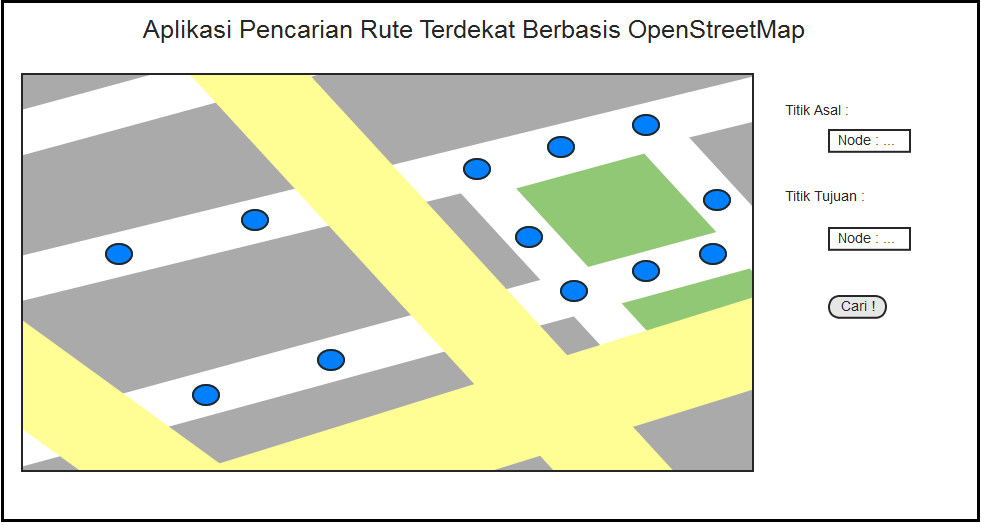
\includegraphics[scale=0.57]{Gambar/mockup_1}
\caption[Rancangan Antar Muka Awal Aplikasi]{Rancangan Antar Muka Awal Aplikasi}
\label{fig:mockup_1}
\end{figure}

Setelah halaman awal terbuka, \textit{User} dapat menekan setiap titik tersebut
dan akan menampilkan \textit{info window} yang memberikan informasi titik
beserta \textit{link}. \textit{User} dapat menekan \textit{link} tersebut untuk
menjadikannya sebagai titik asal ataupun titik tujuan. Rancangan antar muka saat
user memilih titik, dapat dilihat pada Gambar \ref{fig:mockup_2}.
\begin{figure}[h]
\centering
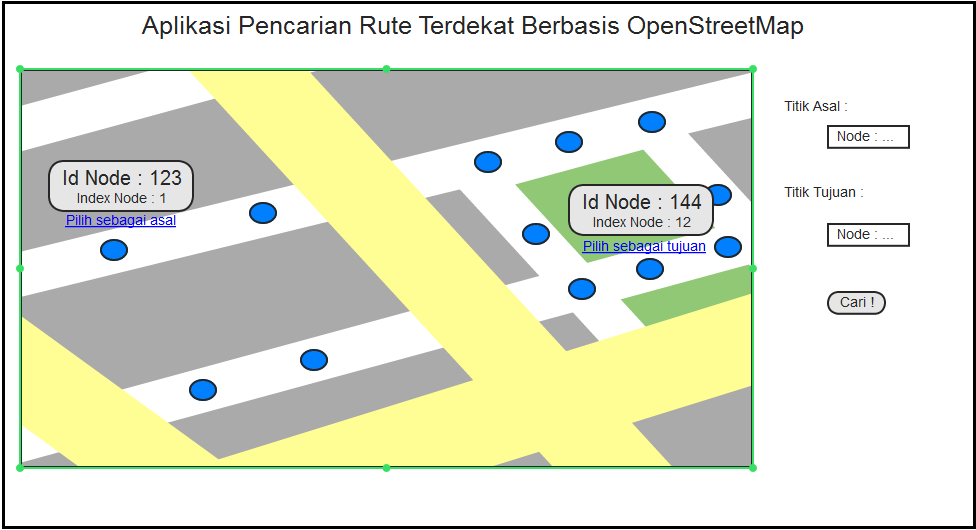
\includegraphics[scale=0.57]{Gambar/mockup_2}
\caption[Rancangan Pemilihan Titik]{Rancangan Pemilihan Titik}
\label{fig:mockup_2}
\end{figure}

Setelah user memilih titik asal dan titik tujuan, user dapat menekan tombol
``Cari!'' untuk melihat rute terdekat antara kedua titik tersebut. Rute tersebut
divisualisasikan dengan menggunakan \textit{polyline} yang berwarna merah.
Rancangan pada tahap ini dapat dilihat pada Gambar \ref{fig:mockup_3}.
\begin{figure}[h]
\centering
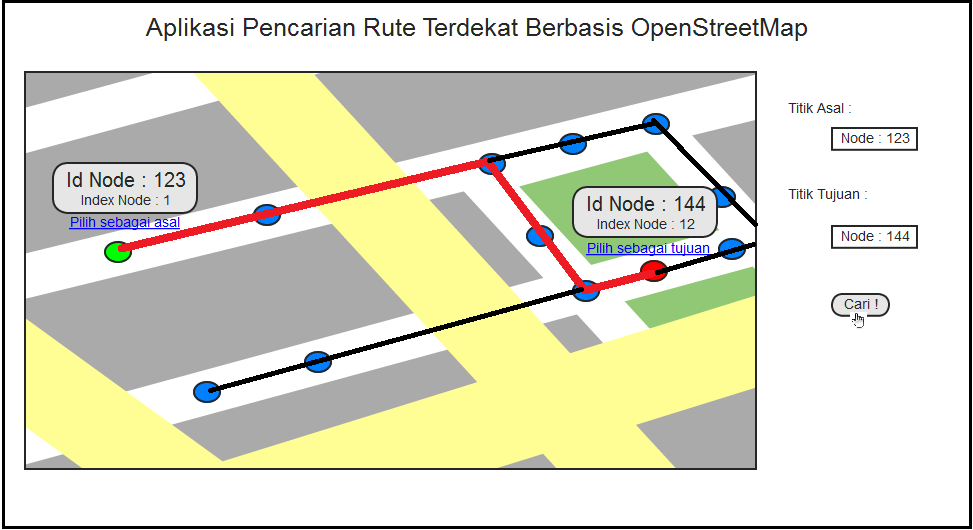
\includegraphics[scale=0.57]{Gambar/mockup_3}
\caption[Rancangan Cari Rute]{Rancangan Cari Rute}
\label{fig:mockup_3}
\end{figure}

\section{Perancangan Kelas}
Pada bagian ini akan dibahas perancangan kelas yang dilakukan untuk aplikasi
yang akan dibangun. Perancangan kelas bertujuan untuk menjelaskan
seluruh atribut dan fungsi yang akan diimplementasikan pada setiap kelas
yang sudah dibahas pada bab analisis. Perancangan kelas yang dibuat dapat 
dilihat pada Gambar \ref{fig:perancangan_kelas}. Berikut ini adalah penjelasan
dari setiap kelas beserta atribut dan fungsi yang digunakan:
\begin{itemize}
  \item Kelas XMLHttpRequest\\
  Kelas ini berfungsi untuk melakukan \textit{load} dokumen OSMXML.
  \begin{itemize}
    \item Fungsi
    \begin{itemize}
      \item open()\\
      Fungsi open() digunakan untuk membuka dokumen OSMXML.
      
      \item send()\\
      Fungsi send() digunakan untuk mengirimkan dokumen OSMXML yang sudah
      dibuka.
    \end{itemize}
  \end{itemize}
  
  \item Kelas Node dan Neighbor\\
  Kedua kelas ini akan menyimpan informasi yang didapatkan dari OSMXML sebagai
  representasi dari graf yaitu \textit{adjacency list}.
  \begin{itemize}
    \item Atribut Kelas Node
    \begin{itemize}
      \item id : int\\
      Atribut id menyimpan id node yang didapatkan dari dokumen OSMXML.
      
      \item adjList : Neighbor\\
      Atribut adjList menyimpan objek Neighbor.
    \end{itemize}
  \end{itemize}
  \begin{itemize}
    \item Atribut Kelas Neighbor
    \begin{itemize}
      \item vertexNum : int\\
      Atribut vertexNum menyimpan index dari node.
      
      \item next : Neighbor\\
      Atribut next menyimpan objek Neighbor.
      
      \item weight : double\\
      Atribut weight menyimpan jarak antar node.
    \end{itemize}
  \end{itemize}
  
  \item Kelas Graph\\
  Kelas ini berfungsi untuk mengubah informasi yang didapatkan dari OSMXML
  menjadi graf.
  \begin{itemize}
    \item Atribut
    \begin{itemize}
      \item adjLists : Array of Node\\
      Atribut adjLists merupakan \textit{array} yang menyimpan objek node.
      
      \item nd : Array\\
      Atribut nd menyimpan informasi berupa id node yang terdapat pada tag way
      di dalam dokumen OSMXML, atribut nd bertipe array.
      
      \item oneway : String\\
      Atribut nd menyimpan informasi berupa \textit{value} dari \textit{key}
      oneway yang terdapat pada tag way di dalam dokumen OSMXML, atribut oneway bertipe String.

\begin{figure}[h]
\centering
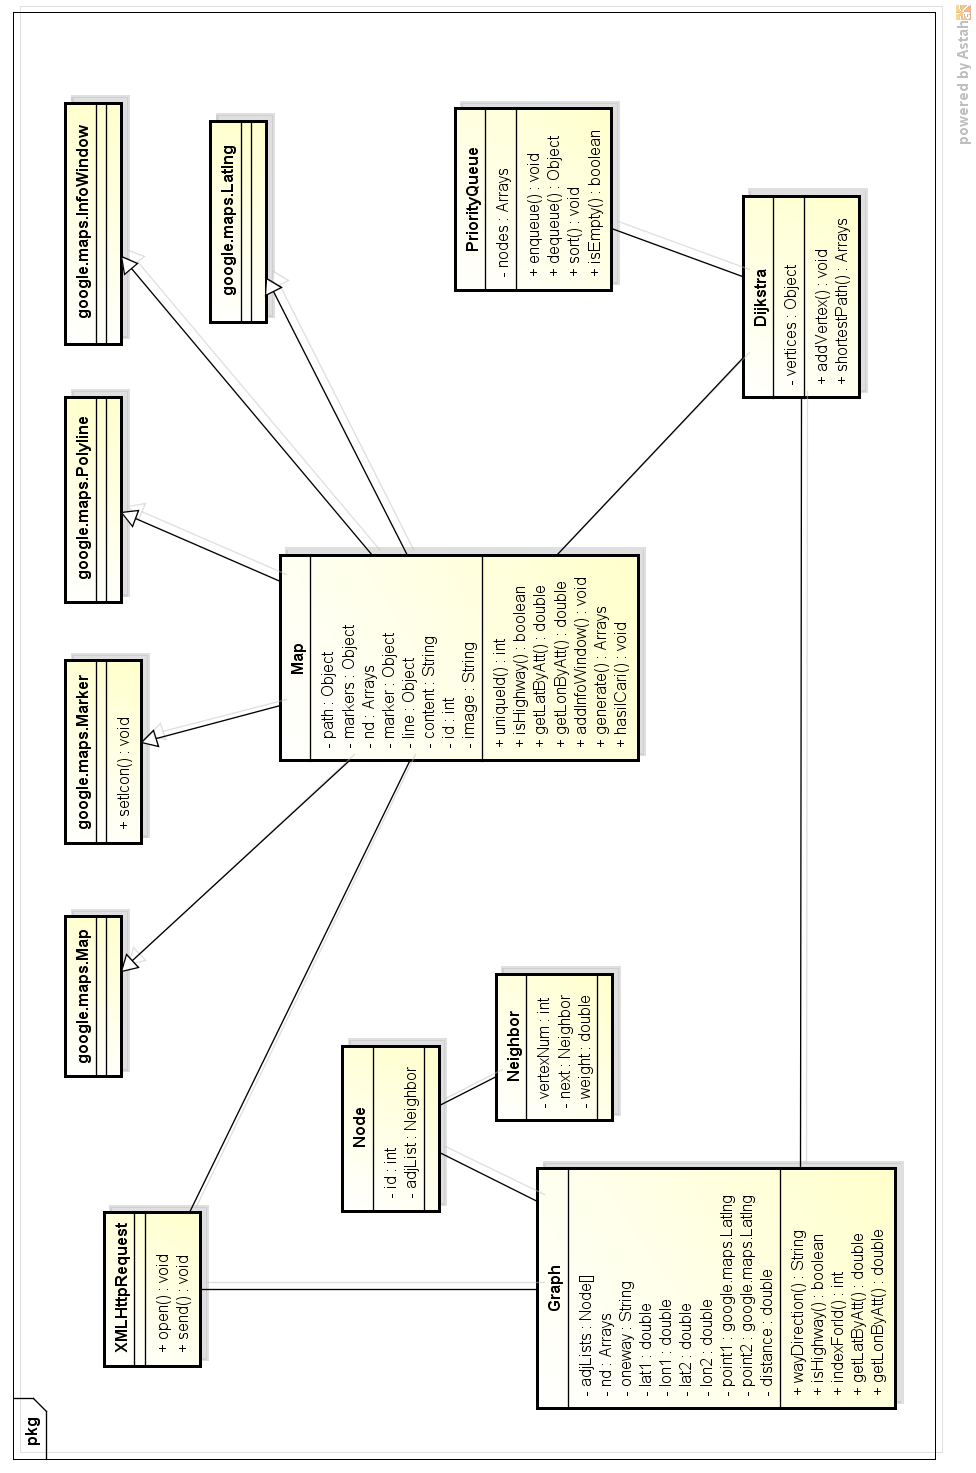
\includegraphics[scale=0.6]{Gambar/perancangan_kelas}
\caption[Diagram Kelas]{Diagram Kelas}
\label{fig:perancangan_kelas}
\end{figure}
\clearpage
    \end{itemize}
  \end{itemize}
  \begin{itemize}
    \item Fungsi
    \begin{itemize}
      \item wayDirection() : String\\
      Fungsi ini digunakan untuk mengetahui arah pada setiap node berdasarkan
      \textit{value} yang terdapat pada OSMXML.
      
      \item isHighway() : boolean\\
      Fungsi ini digunakan untuk melakukan \textit{filter} pada tag way, yaitu
      hanya way yang bertipe ``Highway'' saja yang akan digunakan pada pemodelan
      graf.
      
      \item indexForId() : int\\
      Fungsi ini digunakan untuk mengetahui index node pada graf berdasarkan id
      node.
      
      \item getLatByAtt() : double\\
      Fungsi ini digunakan untuk mendapatkan informasi \textit{latitude} pada
      sebuah node berdasarkan atributnya, yaitu id node.
      
      \item getLonByAtt() : double\\
      Fungsi ini digunakan untuk mendapatkan informasi \textit{longitude} pada
      sebuah node berdasarkan atributnya, yaitu id node.
    \end{itemize}
  \end{itemize}
  
  \item Kelas Map\\
  Kelas ini berfungsi untuk melakukan \textit{generate} peta, visualisasi graf,
  dan visualisasi rute terdekat.
  \begin{itemize}
    \item Atribut
    \begin{itemize}
      \item path : Object\\
      Atribut path adalah variabel yang menyimpan informasi titik koordinat
      dalam bentuk objek, atribut path digunakan untuk pembuatan \textit{marker}
      dan \textit{polyline}.
      
      \item markers : Object\\
      Atribut ini menyimpan seluruh objek \textit{marker}.
      
      \item nd : Arrays\\
      Atribut nd menyimpan informasi berupa id node yang terdapat pada tag way
      di dalam dokumen OSMXML, atribut nd bertipe array.
      
      \item marker : Object\\
      Atribut ini menyimpan objek \textit{marker} untuk ditampilkan pada peta.
      
      \item line : Object\\
      Atribut ini menyimpan objek \textit{polyline} untuk ditampilkan pada peta.
      
      \item content : String\\
      Atribut ini merupakan isi dari \textit{info window} yang disisipkan pada
      setiap marker. Atribut ini berisi id node, index node, \textit{link} titik
      asal, dan \textit{link} titik tujuan.
      
      \item id : int\\
      Atribut ini merupakan id yang digunakan untuk melakukan \textit{generate}
      id pada fungsi uniqueId. 
      
      \item image : String\\
      Atribut ini menyimpan alamat dari \textit{image} atau gambar yang
      digunakan oleh \textit{marker}.
    \end{itemize}
  \end{itemize}
  \begin{itemize}
    \item Fungsi
    \begin{itemize}
      \item uniqueId() : id\\
      Fungsi ini digunakan untuk melakukan \textit{generate} id, id tersebut
      digunakan oleh \textit{marker}.
      
      \item isHighway() : boolean\\
      Fungsi ini digunakan untuk melakukan \textit{filter} pada tag way, hanya
      way yang bertipe ``Highway'' saja yang digunakan. Fungsi ini digunakan
      pada saat pembuatan objek \textit{marker} pada peta.
      
       \item getLatByAtt() : double\\
      Fungsi ini digunakan untuk mendapatkan informasi \textit{latitude} pada
      sebuah node berdasarkan atributnya, yaitu id node.
      
      \item getLonByAtt() : double\\
      Fungsi ini digunakan untuk mendapatkan informasi \textit{longitude} pada
      sebuah node berdasarkan atributnya, yaitu id node.
      
      \item addInfoWindow()\\
      Fungsi ini digunakan untuk menambahkan objek \textit{info window} pada
      setiap \textit{marker}.
      
      \item generate() : Arrays\\
      Fungsi ini digunakan untuk menampilkan secara keseluruhan \textit{marker}
      dan \textit{polyline} pada peta. Fungsi akan mengembalikan
      objek \textit{marker} di dalam bentuk array.
      
      \item hasilCari()\\
      Fungsi ini digunakan untuk melakukan visualisasi rute terdekat menggunakan
      \textit{polyline}.
    \end{itemize}
  \end{itemize}
  
  \item Kelas google.maps.Map\\
  Kelas ini berfungsi untuk membuat objek peta.
  
  \item Kelas google.maps.Marker\\
  Kelas ini berfungsi untuk membuat objek \textit{marker} yang akan digunakan
  sebagai visualisasi node pada peta.
  \begin{itemize}
    \item Fungsi
    \begin{itemize}
      \item SetIcon()\\
      Fungsi ini digunakan untuk mengubah icon dari \textit{marker}.
    \end{itemize}
  \end{itemize}
  
  \item Kelas google.maps.Polyline\\
  Kelas ini berfungsi untuk membuat objek \textit{polyline} yang akan digunakan
  sebagai visualisasi edge pada peta.
  
  \item Kelas google.maps.InfoWindow\\
  Kelas ini berfungsi untuk membuat objek \textit{InfoWindow} yang akan
  disisipkan pada setiap objek \textit{marker}.
  
  \item Kelas google.maps.Latlng\\
  Kelas ini berfungsi untuk membuat objek Latlng. Latlng merupakan objek yang
  berisi informasi koordinat (\textit{latitude} dan \textit{longitude}).
  
  \item Kelas Dijkstra\\
  Kelas ini berfungsi untuk mencari rute terdekat berdasarkan \textit{input}
  titik asal dan titik tujuan.
  \begin{itemize}
    \item Atribut
    \begin{itemize}
      \item nodes : Object\\
      Atribut ini menyimpan informasi node dalam bentuk objek.
    \end{itemize}
  \end{itemize}
  \begin{itemize}
    \item Fungsi
    \begin{itemize}
      \item addNode()\\
      Fungsi ini digunakan untuk menambahkan satu node beserta edgenya.
      
      \item shortestPath() : Arrays\\
      Fungsi ini digunakan untuk pencarian rute terdekat, fungsi akan
      mengembalikan rute atau jalur terpendek dalam bentuk array.
    \end{itemize}
  \end{itemize}
  
  \item Kelas PriorityQueue\\
  Kelas ini merupakan struktur data \textit{priority queue} yang digunakan pada
  kelas dijkstra.
  \begin{itemize}
    \item Atribut
    \begin{itemize}
      \item queue : Array\\
      Atribut ini merupakan \textit{priority queue} dari kelas PriorityQueue.
    \end{itemize}
  \end{itemize}
  \begin{itemize}
    \item Fungsi
    \begin{itemize}
      \item enqueue()\\
      Fungsi ini digunakan untuk menambahkan objek ke dalam \textit{priority
      queue}.
      
      \item dequeue() : Object\\
      Fungsi ini digunakan untuk mengeluarkan objek dari dalam \textit{priority
      queue}.
      
      \item isEmpty() : boolean\\
      Fungsi ini digunakan untuk pengecekan isi dari \textit{priority queue}.
      jika \textit{priority queue} kosong, fungsi akan mengembalikan ``true''
      dan sebaliknya ``false'' jika \textit{priority queue} tidak kosong.
    \end{itemize}
  \end{itemize}
\end{itemize}

\section{Diagram Sekuens}
Diagram sekuens adalah diagram yang digunakan untuk menggambarkan interaksi
antara objek dengan waktu, interaksi tersebut digambarkan dengan grafik dua
dimensi. Kedua dimensi tersebut adalah dimensi horizontal dan dimensi vertikal.
Dimensi horizontal menggambarkan objek yang berperan, sedangkan dimensi
vertikal menggambarkan waktu. Pesan yang dikirimkan oleh objek digambarkan
dengan panah dan pesan balasan dilambangkan dengan panah bergaris putus-putus.
Diagram sekuens mengacu kepada diagram \textit{use case} yang
terdapat pada bab 3, dapat dilihat pada Gambar \ref{fig:usecase}. Berikut ini
adalah diagram sekuens berdasarkan diagram \textit{use case} tersebut:
\begin{enumerate}
  \item Pemilihan Titik Asal\\
  Diagram sekuens untuk pemilihan titik asal dapat dilihat pada Gambar
  \ref{fig:sd_titikAsal}.
\begin{figure}[h]
\centering
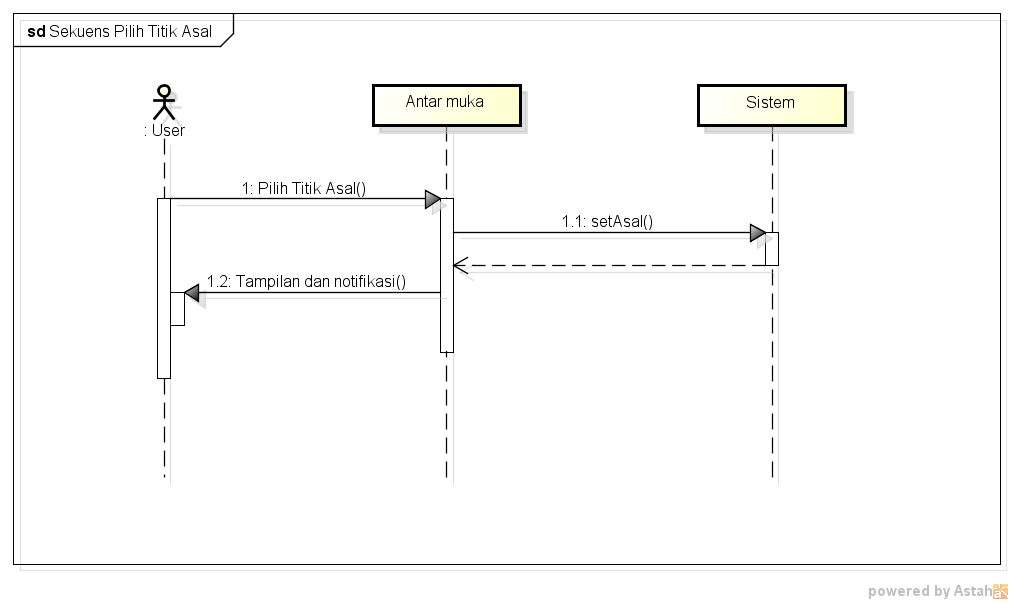
\includegraphics[scale=0.5]{Gambar/sd_titikAsal}
\caption[Diagram Sekuens Pemilihan Titik Asal]{Diagram Sekuens Pemilihan Titik
Asal}
\label{fig:sd_titikAsal}
\end{figure}
  
  \item Pemilihan Titik Tujuan\\
  Diagram sekuens untuk pemilihan titik asal dapat dilihat pada Gambar
  \ref{fig:sd_titikTujuan}.
\begin{figure}[H]
\centering
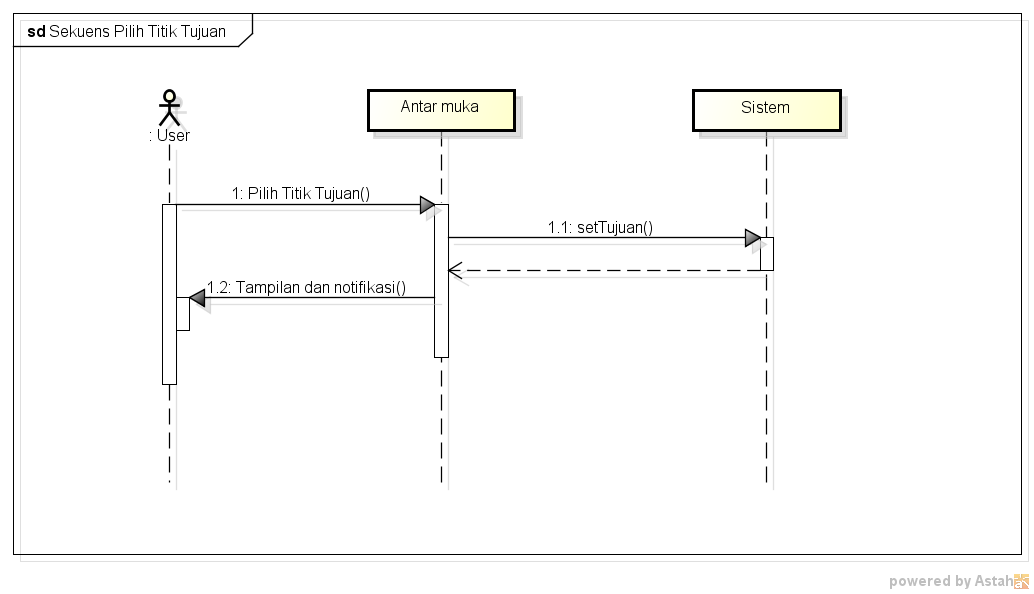
\includegraphics[scale=0.5]{Gambar/sd_titikTujuan}
\caption[Diagram Sekuens Pemilihan Titik Tujuan]{Diagram Sekuens Pemilihan Titik
Tujuan}
\label{fig:sd_titikTujuan}
\end{figure}
  
  \item Pencarian Rute Terdekat\\
  Diagram sekuens untuk pencarian rute terdekat dapat dilihat pada Gambar
  \ref{fig:sd_rute}.
\begin{figure}[h]
\centering
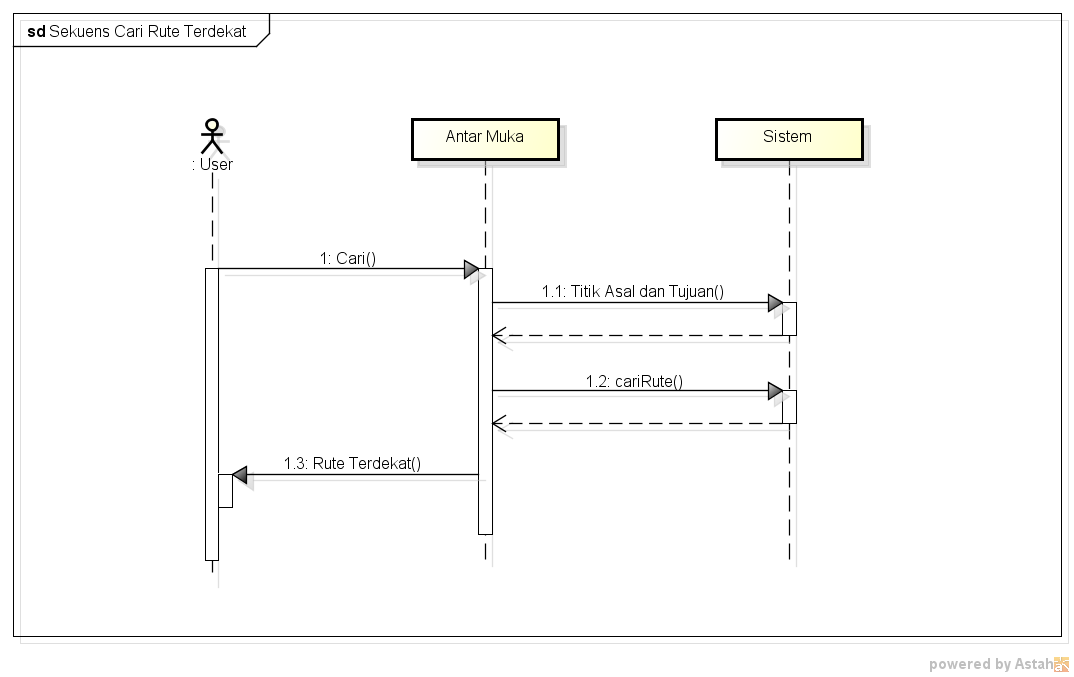
\includegraphics[scale=0.47]{Gambar/sd_rute}
\caption[Diagram Sekuens Pencarian Rute Terdekat]{Diagram Sekuens Pencarian Rute Terdekat}
\label{fig:sd_rute}
\end{figure}
\end{enumerate}}{}
\ifdefstring{\vbabe}{1}{\chapter{Implementasi dan Pengujian}
Pada bagian ini akan dijelaskan tentang implementasi dan pengujian yang
dilakukan. Implementasi adalah tahapan setelah proses perancangan selesai,
rancangan yang sudah dibuat, diimplementasikan menggunakan kode program. Bahasa
pemrograman yang digunakan adalah javascript. Setelah implementasi dilakukan,
akan dilakukan juga beberapa pengujian. Pengujian dilakukan untuk mengetahui
apakah fungsi-fungsi utama aplikasi sudah berjalan dengan baik dan
juga untuk mengetahui kekurangan yang dimiliki aplikasi tersebut.

\section{Implementasi}
Implementasi dilakukan menggunakan bahasa pemrograman javascript, hasil
implementasi adalah dokumen HTML. Berikut ini adalah lingkungan pembangunan
aplikasi pada saat implementasi dilakukan:
\begin{enumerate}
  \item Processor\\
  Intel Core i5-2410M CPU @ 2.30Ghz (4 CPU)
  
  \item Memory\\
  4096MB RAM
  
  \item Display\\
  AMD Radeon HD 6470M
  
  \item Operating System\\
  Windows 7 Ultimate 64-bit
  
  \item Browser\\
  Mozilla Firefox Version 37.0 dan Google Chrome Version 41.0.2272.118 m 
  
  \item Bahasa Pemrograman\\
  Javascript
  
  \item Teks Editor\\
  Notepad++
\end{enumerate}

\section{Pengujian}
Pada subbab ini akan dibahas pengujian yang dilakukan. Pengujian yang dilakukan
dibagi menjadi dua tahap yaitu pengujian fungsional dan pengujian eksperimental.
Pengujian fungsional menguji tampilan antar muka aplikasi beserta method atau
fungsi dasar, sedangkan pengujian eksperimental dilakukan dengan menggunakan
tiga dokumen OSMXML yang berbeda.

\subsection{Pengujian Fungsional}
Pengujian fungsional menguji tampilan antar muka aplikasi beserta method atau
fungsi dasar. Seluruh pengujian fungsional menggunakan dokumen OSMXML
yang bernama ``test.xml'', dokumen ini memiliki batas koordinat yaitu ``<bounds
minlat="-6.9131000" minlon="107.5931000" maxlat="-6.9003000"
maxlon="107.6149000"/>'', cakupan area tersebut berlokasi di Kota Bandung.
Berikut ini adalah daftar fungsi yang diujikan:
\begin{enumerate}
  \item Tampilan antar muka.\\
  Pada tampilan antar muka aplikasi terdapat elemen ``<div>'' sebagai tempat
  untuk menampilkan peta dengan ukuran lebar 75\% dari lebar layar dan tinggi 600px. 
  Di sebelah kanan layar terdapat 2 buah \textit{TextBox} yang menampilkan informasi titik asal
  dan titik tujuan ketika \textit{user} memilih. Selain itu, terdapat 2 buah
  tombol yaitu ``Cari!'' untuk mencari rute terdekat antara kedua titik
  dan tombol kedua adalah ``Reload'' untuk memuat ulang aplikasi. Hasil
  pengujian tampilan antar muka dapat dilihat pada Gambar \ref{fig:pu_antarmuka}.
\begin{figure}[h]
\centering
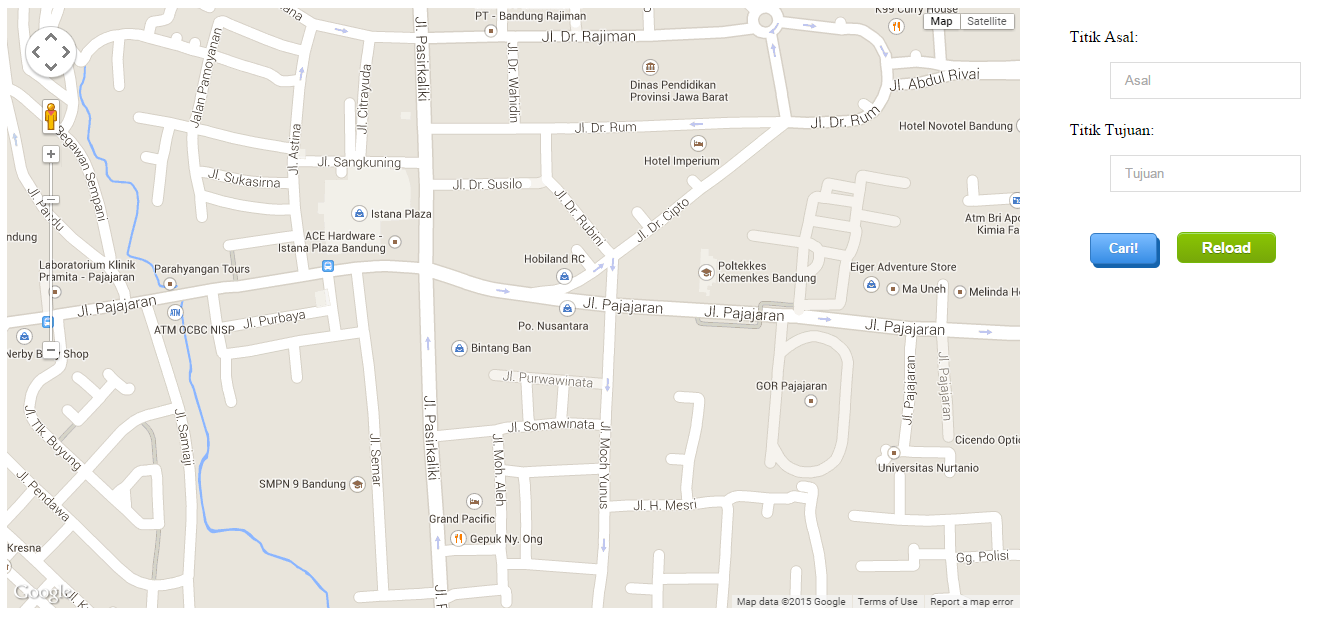
\includegraphics[scale=0.45]{Gambar/pu_antarmuka}
\caption[Pengujian Antar Muka]{Pengujian Antar Muka}
\label{fig:pu_antarmuka}
\end{figure}
  
  \item Fungsi untuk membaca dokumen OSMXML.\\
  Aplikasi mendapatkan informasi dari dokumen OSMXML. Pengujian
  fungsi ini dilakukan untuk memastikan bahwa dokumen OSMXML dapat dibaca dengan
  baik. Pengujian dilakukan dengan cara membandingkan dokumen OSMXML dengan
  informasi yang sudah dibaca. Contoh kasus adalah membandingkan 10 node
  pertama, potongan informasi 10 node pertama pada ``test.xml'' dapat dilihat
  pada Gambar \ref{fig:pu_osmxml2} dan hasil pengujian dapat dilihat pada Gambar
  \ref{fig:pu_osmxml1}. Pada Gambar \ref{fig:pu_osmxml2} menunjukkan bahwa hasil
  pembacaan sama dengan ``test.xml'' pada Gambar \ref{fig:pu_osmxml1}, hal ini
  menunjukkan fungsi untuk membaca dokumen OSMXML sudah berjalan dengan baik.
\begin{figure}[h]
\centering
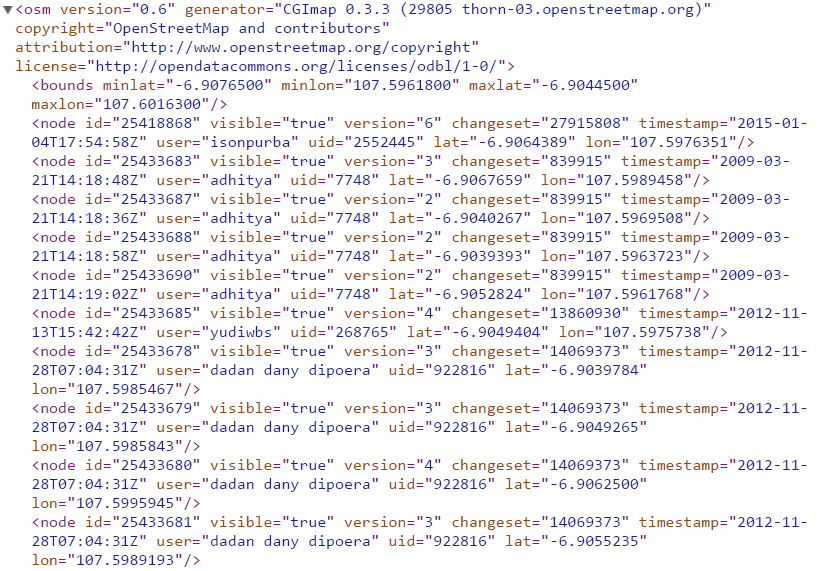
\includegraphics[scale=0.7]{Gambar/pu_osmxml2}
\caption[Dokumen test.xml]{Dokumen test.xml}
\label{fig:pu_osmxml2}
\end{figure}

\begin{figure}[h]
\centering
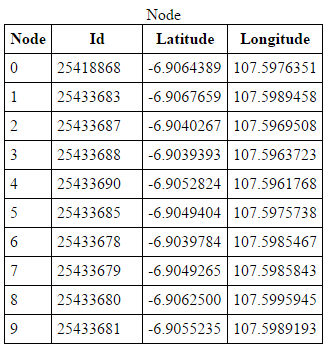
\includegraphics[scale=1]{Gambar/pu_osmxml1}
\caption[Pengujian Fungsi OSMXML]{Pengujian Fungsi OSMXML}
\label{fig:pu_osmxml1}
\end{figure}
\clearpage

  \item Fungsi untuk mengukur jarak antara dua titik.\\
  Pengukuran jarak antara dua titik menggunakan \textit{geometry spherical}.
  Contoh kasus adalah mencari jarak setiap titik yang terdapat pada tag way
  dengan id 190605660, hasil pengujian dapat dilihat pada Gambar
  \ref{fig:pu_jarak1} dan \ref{fig:pu_jarak2}.
\begin{figure}[h]
\centering
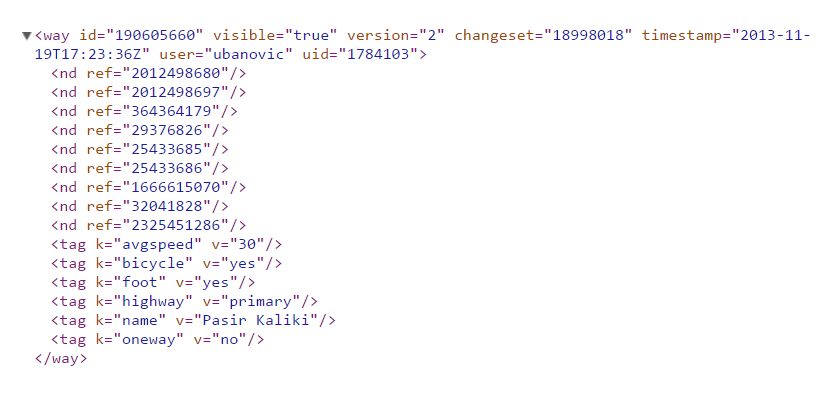
\includegraphics[scale=0.7]{Gambar/pu_jarak1}
\caption[Dokumen test.xml]{Dokumen test.xml}
\label{fig:pu_jarak1}
\end{figure}

\begin{figure}[h]
\centering
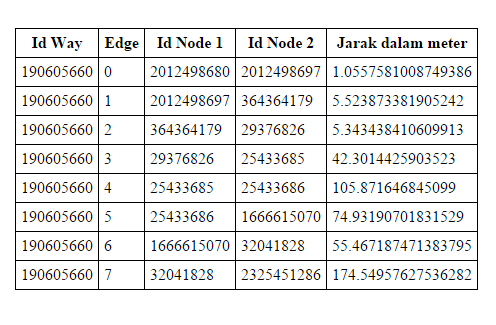
\includegraphics[scale=1]{Gambar/pu_jarak2}
\caption[Pengujian Jarak]{Pengujian Jarak}
\label{fig:pu_jarak2}
\end{figure}

\item Fungsi untuk mengubah informasi OSMXML menjadi graf.
\begin{figure}[h]
\centering
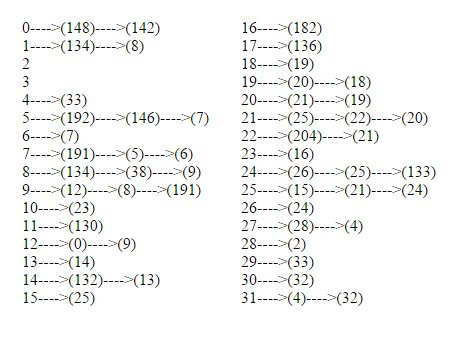
\includegraphics[scale=1]{Gambar/pu_graf}
\caption[Pengujian Fungsi OSMXML Menjadi Graf]{Pengujian Fungsi OSMXML Menjadi Graf}
\label{fig:pu_graf}
\end{figure}\\
  Informasi yang didapatkan dari OSMXML, selanjutnya diubah menjadi graf.
  Pengujian dilakukan dengan mengubah seluruh ``test.xml'' menjadi graf
  menggunakan \textit{adjacency list}. Berikut hasil pengujian, dapat dilihat
  pada Gambar \ref{fig:pu_graf}. Pada Gambar \ref{fig:pu_graf} hanya ditampilkan
  hingga 32 node, hal ini dikarenakan ``test.xml'' memiliki 207 buah node dan 
  terlalu banyak jika ditampilkan seluruhnya.
  
  \item Fungsi untuk melakukan visualisasi.\\
  Fungsi ini menggambarkan setiap node menggunakan \textit{marker} dan
  setiap edge menggunakan \text{polyline} pada peta, hasil pengujian dapat
  dilihat pada Gambar \ref{fig:pu_visual}.
\begin{figure}[h]
\centering
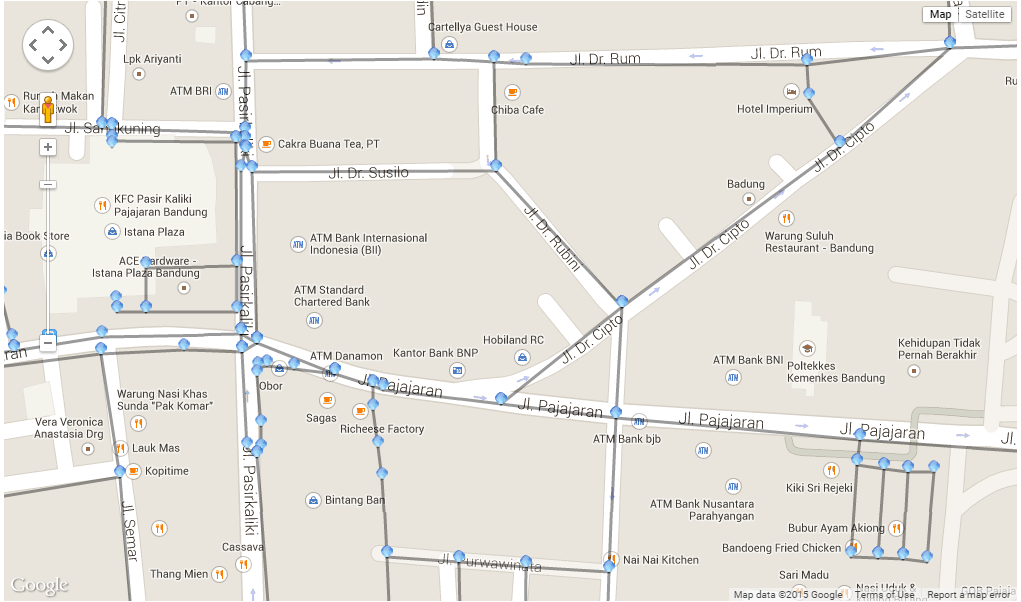
\includegraphics[scale=0.5]{Gambar/pu_visual}
\caption[Pengujian Fungsi Visualisasi]{Pengujian Fungsi Visualisasi}
\label{fig:pu_visual}
\end{figure}

  \item Fungsi untuk memilih titik asal dan titik tujuan.\\
  Pengujian dilakukan dengan memilih titik asal dan titik tujuan. Titik asal
  yang sudah dipilih berganti \textit{icon} dengan warna hijau dan titik tujuan
  yang sudah dipilih berganti \textit{icon} dengan warna merah. Informasi
  Id Node dari kedua titik yang sudah dipilih, ditampilkan di sebelah kanan
  layar. Hasil pengujian dapat dilihat pada Gambar \ref{fig:pu_titik}.
\begin{figure}[h]
\centering
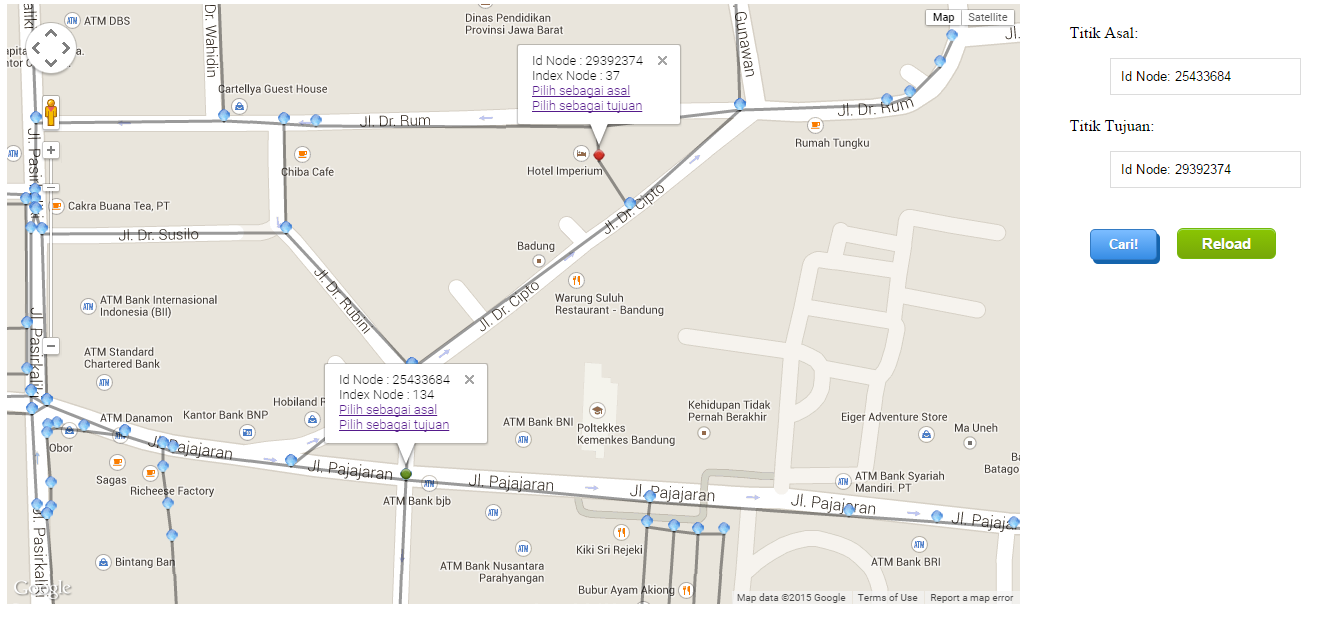
\includegraphics[scale=0.45]{Gambar/pu_titik}
\caption[Pengujian Titik Asal dan Tujuan]{Pengujian Titik Asal dan Tujuan}
\label{fig:pu_titik}
\end{figure}
  
  \item Fungsi untuk mencari rute terdekat antar dua titik menggunakan
  algoritma dijkstra.\\
  Pengujian dilakukan dengan contoh kasus mencari rute terdekat dari titik asal
  (id node : 29356381, index node : 16) ke titik tujuan (id node : 25500626,
  index node : 11), hasil pengujian dapat dilihat pada Gambar \ref{fig:pu_rute}.
\begin{figure}[h]
\centering
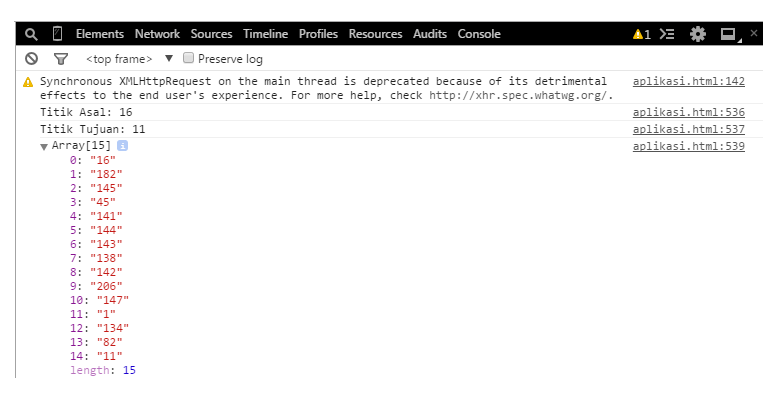
\includegraphics[scale=0.8]{Gambar/pu_rute}
\caption[Pengujian Rute Terdekat]{Pengujian Rute Terdekat}
\label{fig:pu_rute}
\end{figure}

  \item Fungsi untuk visualisasi rute terdekat.\\
  Pengujian dilakukan dengan contoh kasus yang sama pada fungsi pencari rute
  terdekat, rute terdekat digambarkan dengan \textit{polyline} berwarna
  merah. Hasil pengujian dapat dilihat pada Gambar \ref{fig:pu_visualrute}.
\begin{figure}[h]
\centering
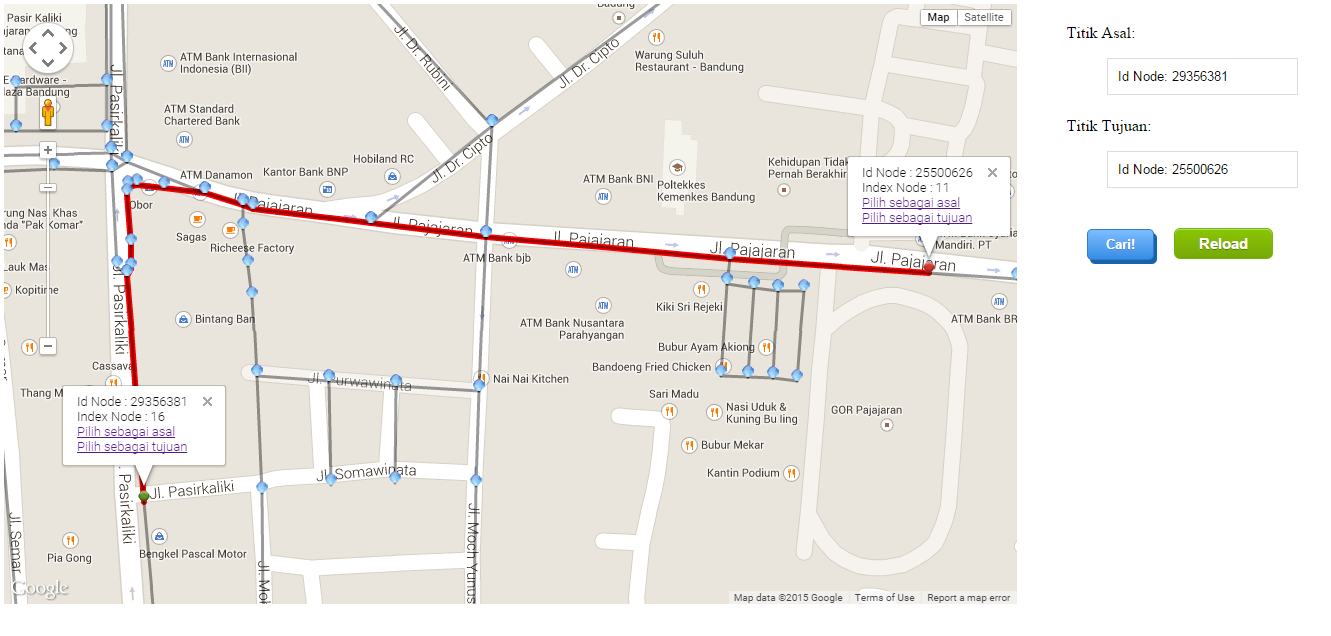
\includegraphics[scale=0.45]{Gambar/pu_visualrute}
\caption[Pengujian Visualisasi Rute Terdekat]{Pengujian Visualisasi Rute
Terdekat}
\label{fig:pu_visualrute}
\end{figure}
\end{enumerate}

\subsection{Pengujian Eksperimental}
Pengujian eksperimental dilakukan dengan menggunakan tiga dokumen OSMXML yang
berbeda. Ketiga dokumen tersebut diberi nama bandung1.xml, bandung2.xml, dan
bandung3.xml, berikut ini adalah cakupan area dari ketiga OSMXML tersebut:
\begin{enumerate}
  \item Bandung 1
  \begin{itemize}
    \item Batas Atas : -6.9044500
    
    \item Batas Bawah : -6.9076500
    
    \item Batas Kiri : 107.5961800
    
    \item Batas Kanan : 107.6016300
  \end{itemize}

  \item Bandung 2
  \begin{itemize}
    \item Batas Atas : -6.9003000
    
    \item Batas Bawah : -6.9131000
    
    \item Batas Kiri : 107.5931000
    
    \item Batas Kanan : 107.6149000
  \end{itemize}
  
  \item Bandung 3
  \begin{itemize}
    \item Batas Atas : -6.8194
    
    \item Batas Bawah : -6.9959
    
    \item Batas Kiri : 107.553
    
    \item Batas Kanan : 107.745
  \end{itemize}
\end{enumerate}

\setcounter{secnumdepth}{3}
\setcounter{tocdepth}{3}
\subsubsection{Pengujian Eksperimental Bandung 1}
\begin{figure}[h]
\centering
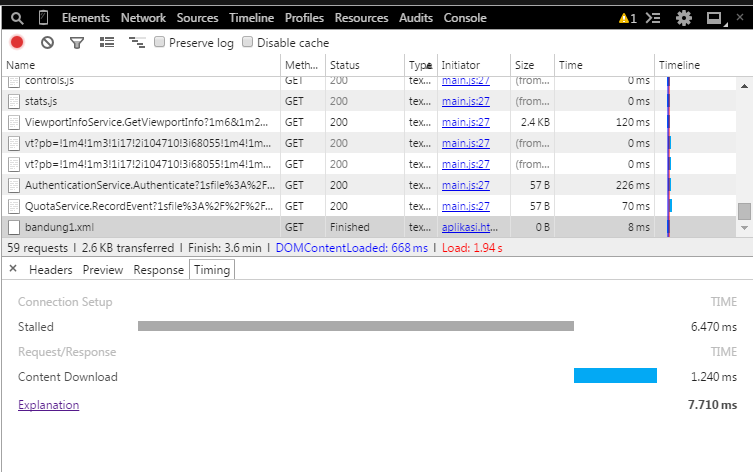
\includegraphics[scale=0.75]{Gambar/pu_bandung1}
\caption[Pengujian Bandung 1]{Pengujian Bandung 1}
\label{fig:pu_bandung1}
\end{figure}
Pengujian dilakukan dengan melihat waktu \textit{load} ``bandung1.xml''
(ukuran \textit{file} sebesar 98Kb), hasil pengujian dapat dilihat pada Gambar
\ref{fig:pu_bandung1}.
Pada Gambar \ref{fig:pu_bandung1} menunjukkan total waktu yang dibutuhkan untuk 
melakukan \textit{load} ``bandung1.xml'' adalah 7.710ms. Berikut ini
adalah aplikasi yang menggunakan dokumen ``bandung1.xml'' dapat dilihat pada
Gambar \ref{fig:bandung1_load}.
\begin{figure}[h]
\centering
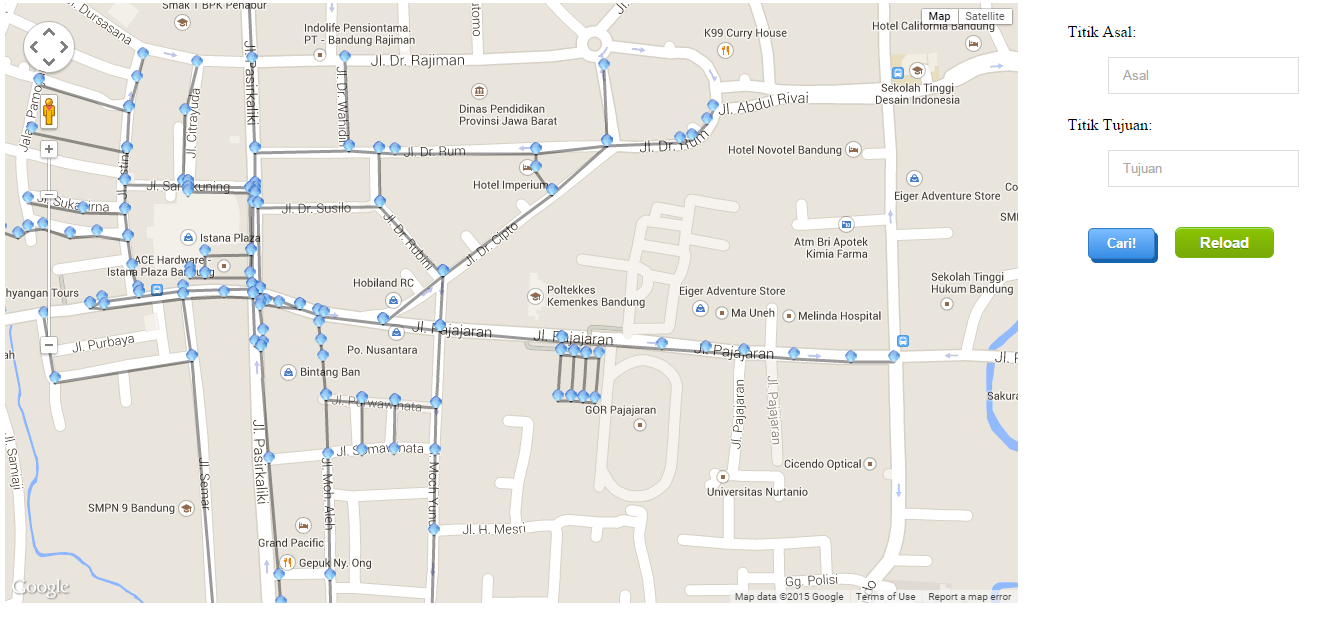
\includegraphics[scale=0.45]{Gambar/bandung1_load}
\caption[Pengujian Bandung 1]{Pengujian Bandung 1}
\label{fig:bandung1_load}
\end{figure}\\
Setelah melakukan \textit{load} aplikasi menggunakan ``bandung1.xml'', pengujian
dilanjutkan dengan mencari rute terdekat dari titik asal (Id Node : 25433686,
Index Node : 192) ke titik tujuan (Id Node : 2325451571, Index Node : 198).
\begin{figure}[h]
\centering
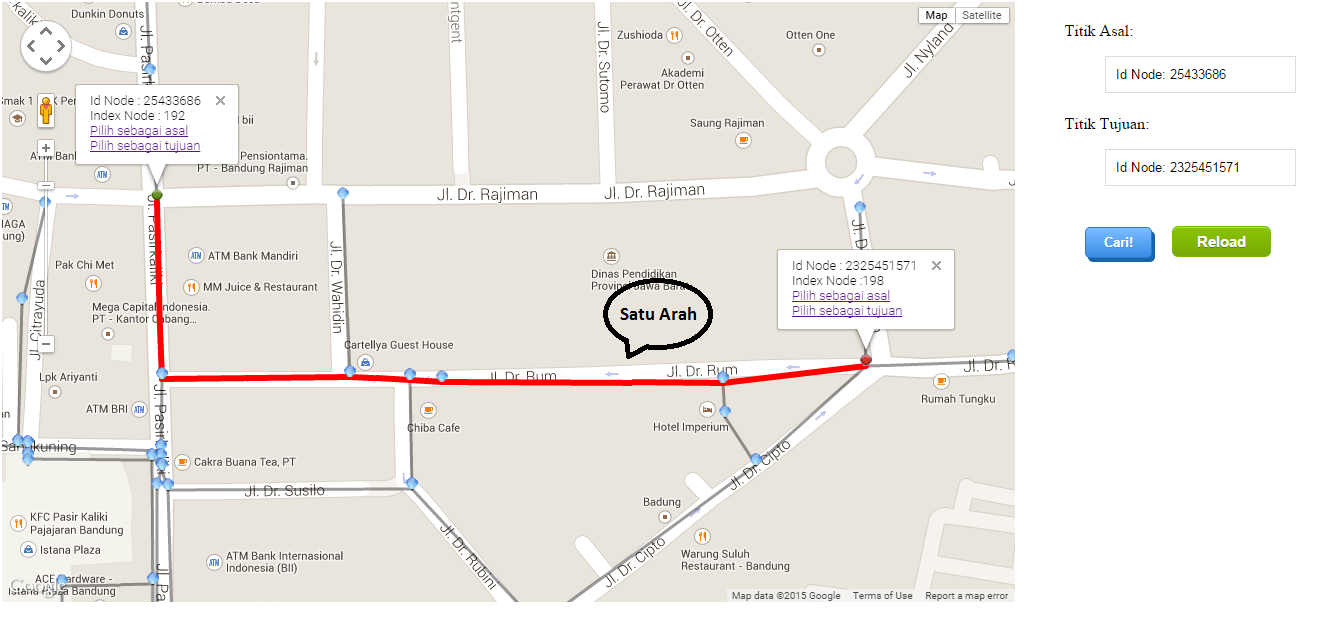
\includegraphics[scale=0.45]{Gambar/pu_bandung1_rute}
\caption[Pengujian Bandung 1]{Pengujian Bandung 1}
\label{fig:pu_bandung1_rute}
\end{figure}
Pada Gambar \ref{fig:pu_bandung1_rute} ditemukan \textit{bug} yaitu aplikasi
menunjukkan rute terdekat (dalam kasus pengujian melalui Jl. Dr Rum) walaupun
rute tersebut melawan arah (pada peta Google Maps menunjukkan bahwa Jl. Dr Rum
adalah jalan satu arah). Setelah dilakukan penelitian lebih lanjut, ternyata kesalahan
ditemukan pada dokumen OSMXML yaitu ``bandung1.xml'' yang tidak memberikan
informasi ``oneway'', sehingga aplikasi memasukkan informasi yang salah tersebut
ke dalam graf sebagai jalan dua arah. Berikut ini adalah potongan dokumen
``bandung1.xml'' yang memberikan informasi Jl. Dr Rum, dapat dilihat pada Gambar
\ref{fig:bandung1_xml} 
\begin{figure}[h]
\centering
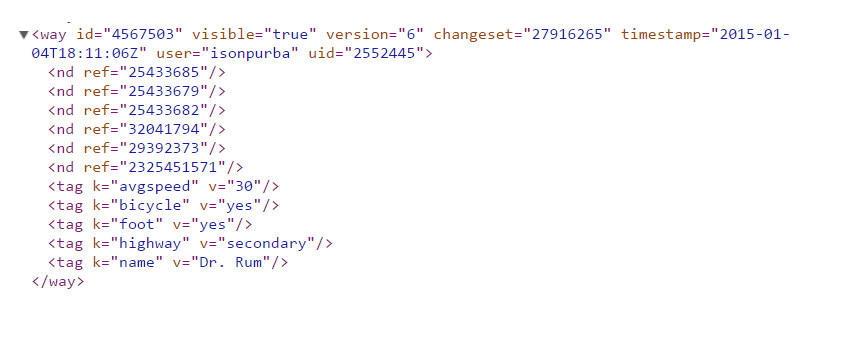
\includegraphics[scale=0.7]{Gambar/bandung1_xml}
\caption[bandung1.xml]{bandung1.xml}
\label{fig:bandung1_xml}
\end{figure}

\subsubsection{Pengujian Eksperimental Bandung 2}
Pengujian dilakukan dengan melihat waktu \textit{load} ``bandung2.xml'' (ukuran
\textit{file} sebesar 821Kb), hasil pengujian dapat dilihat pada Gambar
\ref{fig:pu_bandung2}. Pada Gambar \ref{fig:pu_bandung2} menunjukkan total waktu yang dibutuhkan untuk 
melakukan \textit{load} ``bandung2.xml'' adalah 70.460ms. 
\begin{figure}[h]
\centering
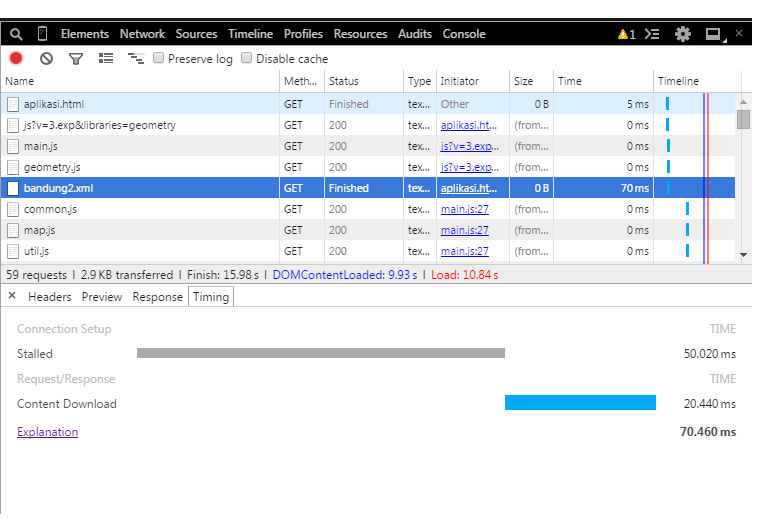
\includegraphics[scale=0.8]{Gambar/pu_bandung2}
\caption[Pengujian Bandung 2]{Pengujian Bandung 2}
\label{fig:pu_bandung2}
\end{figure}
Berikut ini adalah aplikasi yang menggunakan dokumen ``bandung2.xml'' dapat
dilihat pada Gambar \ref{fig:bandung2_load}.
\begin{figure}[h]
\centering
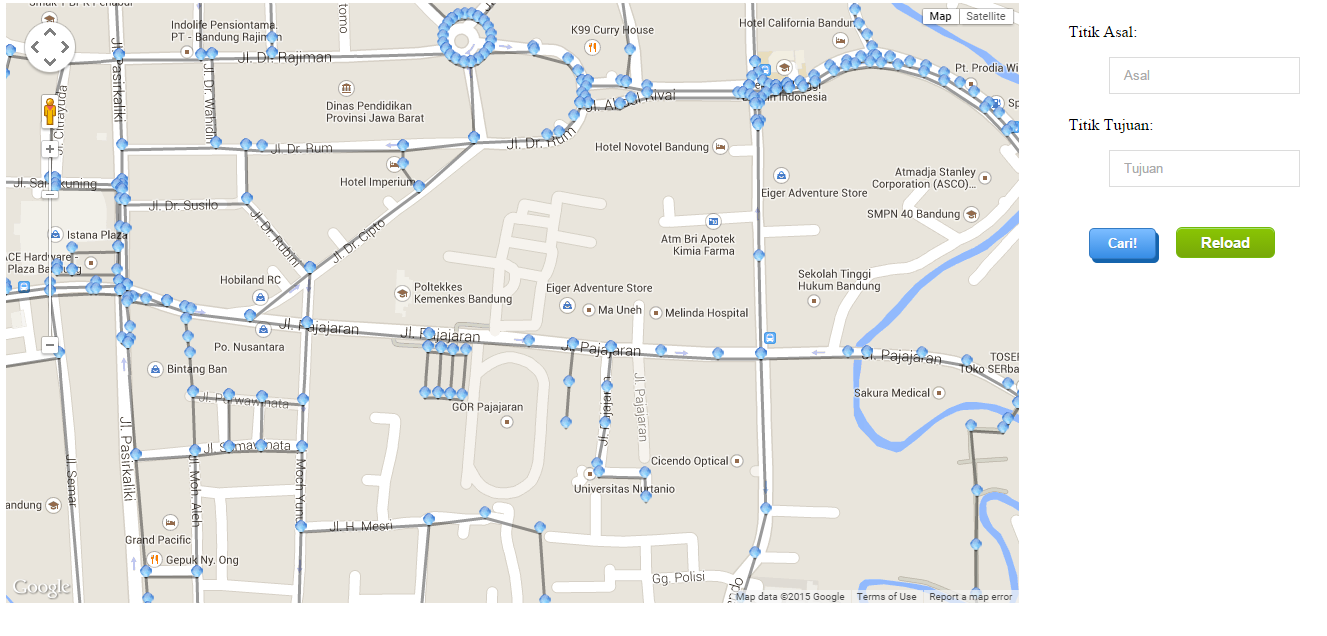
\includegraphics[scale=0.45]{Gambar/bandung2_load}
\caption[Pengujian Bandung 2]{Pengujian Bandung 2}
\label{fig:bandung2_load}
\end{figure}
Setelah melakukan \textit{load} aplikasi menggunakan ``bandung2.xml'', pengujian
dilanjutkan dengan mencari rute terdekat dari titik asal (Id Node : 29356503,
Index Node : 47) ke titik tujuan (Id Node : 1700554920, Index Node : 1163).
Hasil pengujian dapat dilihat pada Gambar \ref{fig:pu_bandung2_rute}.
\clearpage
\begin{figure}[h]
\centering
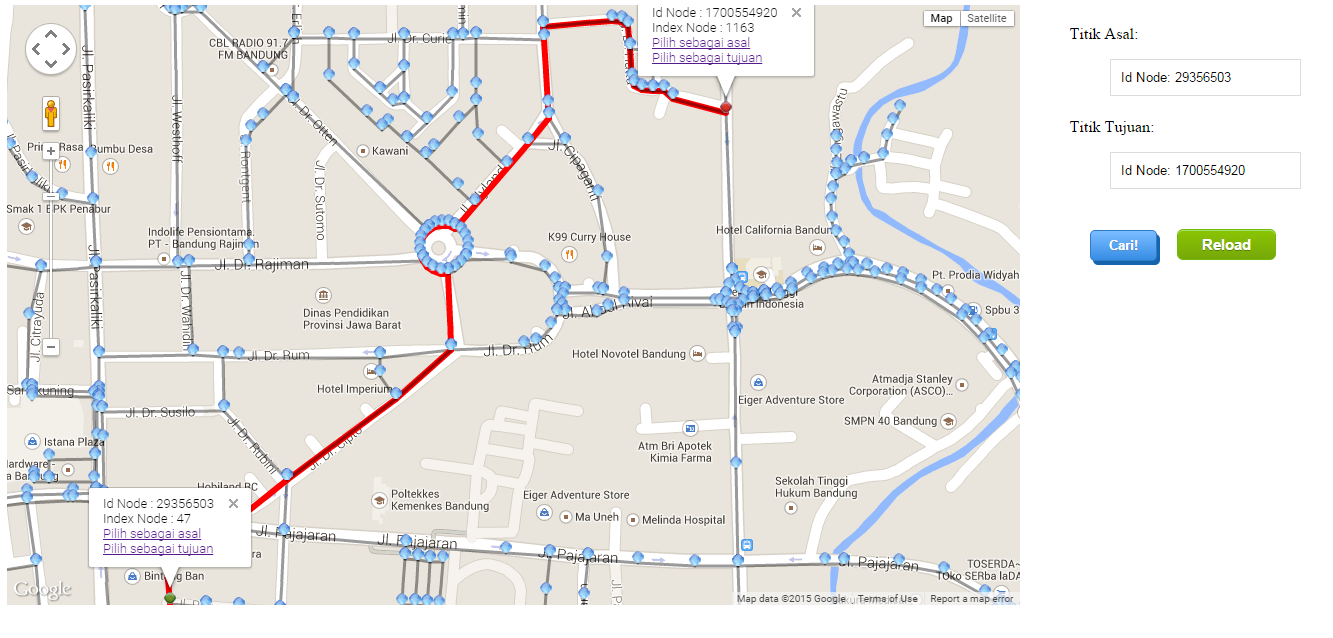
\includegraphics[scale=0.45]{Gambar/pu_bandung2_rute}
\caption[Pengujian Bandung 2]{Pengujian Bandung 2}
\label{fig:pu_bandung2_rute}
\end{figure}

\subsubsection{Pengujian Eksperimental Bandung 3}
Pengujian dilakukan dengan melihat waktu \textit{load} ``bandung3.xml'' (ukuran
\textit{file} sebesar 17,631Kb). Dokumen ``bandung3.xml'' adalah OSMXML yang
mencakup seluruh wilayah Kota Bandung, berdasarkan pengujian yang telah dilakukan, aplikasi tidak berhasil untuk 
menggunakan ``bandung3.xml''. Hal ini disebabkan oleh dokumen ``bandung3.xml
yang terlalu besar'', waktu \textit{load} yang terlalu lama sehingga browser 
menampilkan kotak dialog yang dapat dilihat pada Gambar
\ref{fig:pu_bandung3}.
\begin{figure}[h]
\centering
\includegraphics[scale=1]{Gambar/pu_bandung3}
\caption[Pengujian Bandung 3]{Pengujian Bandung 3}
\label{fig:pu_bandung3}
\end{figure}

\subsubsection{Hasil Pengujian}
Berdasarkan pengujian eksperimental yang telah dilakukan, diketahui beberapa hal
yaitu:
\begin{enumerate}
  \item \textit{Load} dokumen OSMXML\\
  Hasil pengujian ketiga dokumen OSMXML dapat dilihat pada Tabel
  \ref{tab:doc_xml}.
\begin{table}[h]
\centering
\caption{Dokumen OSMXML} 
\label{tab:doc_xml}
\begin{tabular}{|c|c|c|c|c|}
\hline
          & Ukuran File & Waktu Load & Jumlah Node & Jumlah Edge \\ \hline
Bandung 1 & 98 Kb       & 7.710 ms   & 208         & 141         \\ \hline
Bandung 2 & 821 Kb      & 70.460 ms  & 2680        & 1073        \\ \hline
Bandung 3 & 17,631 Kb   & -          & -           & -           \\ \hline
\end{tabular}
\end{table}

  Berdasarkan pengujian tersebut, ``bandung3.xml" tidak berhasil dibuka
  karena ukurannya yang terlalu besar dan diketahui bawah semakin besar dokumen
  OSMXML, semakin besar pula waktu \textit{load} yang diperlukan.
  
  \item Bug\\
  Bug ditemukan ketika pengujian berlangsung, yaitu rute terdekat yang
  ditunjukkan oleh aplikasi melawan arus jalan, hal ini disebabkan oleh dokumen
  OSMXML yang tidak memberikan informasi ``oneway''.
\end{enumerate}











}{}
\ifdefstring{\vbabf}{1}{\chapter{Kesimpulan dan Saran}
\section{Kesimpulan}
\begin{enumerate}
  \item OSMXML merupakan data peta yang disediakan oleh situs
  OpenStreetMap dalam bentuk dokumen XML. OSMXML memiliki informasi node dan
  edge, informasi tersebut dapat dibaca menggunakan Javascript dan dimodelkan 
  ke dalam bentuk graf berarah, graf tersebut dimodelkan menggunakan
  \textit{adjacency list}.
  
  \item Algoritma Dijkstra dapat mencari rute terdekat pada graf berarah.
  Aplikasi menggunakan algoritma dijkstra pada graf berarah yang sudah berhasil
  dimodelkan.
  
  \item Visualisasi graf dapat dibuat menggunakan Google Maps Javascript API.
  Aplikasi menampilkan informasi node dan edge pada OSMXML dengan objek
  \textit{marker} dan \textit{polyline}. Rute terdekat didapatkan dari hasil
  algoritma dijkstra yang telah diimplementasikan dan divisualkan dengan
  \textit{polyline}.
\end{enumerate}

\section{Saran}
\begin{enumerate}
\item OSMXML memiliki informasi selain node dan edge yaitu ``relation''.
\textit{Relation} menyimpan informasi seperti rute angkutan, rute bus, rute
\textit{hiking}, dan lain-lain. Untuk pengembangan aplikasi yang juga
menggunakan data peta dari OpenStreetMap dapat menggunakan informasi tersebut,
sehingga tidak hanya rute mengemudi saja, tetapi juga dapat mencari rute
terdekat angkutan, bus, atau rute lainnya.

\item Informasi yang didapatkan dari OSMXML dapat dilakukan \textit{preprocess}
terlebih dahulu, sehingga kecepatan proses lebih cepat.
\end{enumerate}}{}
\ifdefstring{\vbabg}{1}{\include{Bab/bab7}}{}
\ifdefstring{\vbabh}{1}{\include{Bab/bab8}}{}
\ifdefstring{\vbabi}{1}{\include{Bab/bab9}}{}

\bibliographystyle{ieeetr}
\bibliography{pustaka}

\appendix
\apptoc

\tampillmp{\vlmp}
\ifdefstring{\vlmpa}{1}{\chapter{Kode Program}
\label{kode_program}

%selalu gunakan single spacing untuk source code !!!!!
\singlespacing 
% language: bahasa dari kode program
% terdapat beberapa pilihan : Java, C, C++, PHP, Matlab, R, dll
%
% basicstyle : ukuran font untuk kode program
% terdapat beberapa pilihan : tiny, scriptsize, footnotesize, dll
%
% caption : nama yang akan ditampilkan di dokumen akhir, lihat contoh
\lstset{basicstyle=\tiny}
\begin{lstlisting}[caption=aplikasi.html]
<!DOCTYPE html>
<html>
<head>
<script src="https://maps.googleapis.com/maps/api/js?v=3.exp&libraries=geometry"></script>

</head>
<style>
.style-1 input[type="text"] {
  padding: 10px;
  border: solid 1px #dcdcdc;
  transition: box-shadow 0.3s, border 0.3s;
}

.style-1 input[type="text"]:focus,
.style-1 input[type="text"].focus {
  border: solid 1px #707070;
  box-shadow: 0 0 5px 1px #969696;
}

.cari {
	-moz-box-shadow: 3px 4px 0px 0px #1564ad;
	-webkit-box-shadow: 3px 4px 0px 0px #1564ad;
	box-shadow: 3px 4px 0px 0px #1564ad;
	background:-webkit-gradient(linear, left top, left bottom, color-stop(0.05, #79bbff), color-stop(1, #378de5));
	background:-moz-linear-gradient(top, #79bbff 5%, #378de5 100%);
	background:-webkit-linear-gradient(top, #79bbff 5%, #378de5 100%);
	background:-o-linear-gradient(top, #79bbff 5%, #378de5 100%);
	background:-ms-linear-gradient(top, #79bbff 5%, #378de5 100%);
	background:linear-gradient(to bottom, #79bbff 5%, #378de5 100%);
	filter:progid:DXImageTransform.Microsoft.gradient(startColorstr='#79bbff', endColorstr='#378de5',GradientType=0);
	background-color:#79bbff;
	-moz-border-radius:5px;
	-webkit-border-radius:5px;
	border-radius:5px;
	border:1px solid #337bc4;
	display:inline-block;
	cursor:pointer;
	color:#ffffff;
	font-family:arial;
	font-size:13px;
	font-weight:bold;
	padding:7px 18px;
	text-decoration:none;
	text-shadow:0px 1px 0px #528ecc;
}

.cari:hover {
	background:-webkit-gradient(linear, left top, left bottom, color-stop(0.05, #378de5), color-stop(1, #79bbff));
	background:-moz-linear-gradient(top, #378de5 5%, #79bbff 100%);
	background:-webkit-linear-gradient(top, #378de5 5%, #79bbff 100%);
	background:-o-linear-gradient(top, #378de5 5%, #79bbff 100%);
	background:-ms-linear-gradient(top, #378de5 5%, #79bbff 100%);
	background:linear-gradient(to bottom, #378de5 5%, #79bbff 100%);
	filter:progid:DXImageTransform.Microsoft.gradient(startColorstr='#378de5', endColorstr='#79bbff',GradientType=0);
	background-color:#378de5;
}

.cari:active {
	position:relative;
	top:1px;
}

.reload {
	-moz-box-shadow:inset 0px 1px 0px 0px #a4e271;
	-webkit-box-shadow:inset 0px 1px 0px 0px #a4e271;
	box-shadow:inset 0px 1px 0px 0px #a4e271;
	background:-webkit-gradient(linear, left top, left bottom, color-stop(0.05, #89c403), color-stop(1, #77a809));
	background:-moz-linear-gradient(top, #89c403 5%, #77a809 100%);
	background:-webkit-linear-gradient(top, #89c403 5%, #77a809 100%);
	background:-o-linear-gradient(top, #89c403 5%, #77a809 100%);
	background:-ms-linear-gradient(top, #89c403 5%, #77a809 100%);
	background:linear-gradient(to bottom, #89c403 5%, #77a809 100%);
	filter:progid:DXImageTransform.Microsoft.gradient(startColorstr='#89c403', endColorstr='#77a809',GradientType=0);
	background-color:#89c403;
	-moz-border-radius:6px;
	-webkit-border-radius:6px;
	border-radius:6px;
	border:1px solid #74b807;
	display:inline-block;
	cursor:pointer;
	color:#ffffff;
	font-family:arial;
	font-size:15px;
	font-weight:bold;
	padding:6px 24px;
	text-decoration:none;
	text-shadow:0px 1px 0px #528009;
}

.reload:hover {
	background:-webkit-gradient(linear, left top, left bottom, color-stop(0.05, #77a809), color-stop(1, #89c403));
	background:-moz-linear-gradient(top, #77a809 5%, #89c403 100%);
	background:-webkit-linear-gradient(top, #77a809 5%, #89c403 100%);
	background:-o-linear-gradient(top, #77a809 5%, #89c403 100%);
	background:-ms-linear-gradient(top, #77a809 5%, #89c403 100%);
	background:linear-gradient(to bottom, #77a809 5%, #89c403 100%);
	filter:progid:DXImageTransform.Microsoft.gradient(startColorstr='#77a809', endColorstr='#89c403',GradientType=0);
	background-color:#77a809;
}

.reload:active {
	position:relative;
	top:1px;
}
</style>
<body>
<div id="googleMap" style="width:75%;height:600px;float:left"></div>
<div id="cari" style="width:25%;height:60px;float:left">
<div style="margin-left:50px;margin-top:20px">
	<table style="border:1">
		<tr>
			<label>Titik Asal:</label>
		</tr>
		<tr>
			<ul class="input-list style-1 clearfix">
				<input type="text" id="asal" placeholder=" Asal ">
			</ul>
		</tr>
	</table>
</div>
<div style="margin-left:50px">
<table>
	<tr>
		<label>Titik Tujuan:</label>
	</tr>
	<tr>
		<ul class="input-list style-1 clearfix">
            <input type="text" id="tujuan" placeholder=" Tujuan ">
        </ul>
	</tr>
	
	<tr>
		<label>Total Jarak Tempuh:</label>
	</tr>
	<tr>
		<ul class="input-list style-1 clearfix">
            <input type="text" id="jarak" placeholder="  ">
        </ul>
	</tr>
	<tr>
		<ul class="input-list style-1 clearfix">
            <input type="text" id="kmjarak" placeholder="  ">
        </ul>
	</tr>
	
	<tr>
		<label>Lama Pencarian:</label>
	</tr>
	<tr>
		<ul class="input-list style-1 clearfix">
            <input type="text" id="waktu" placeholder="  ">
        </ul>
	</tr>
</table>
</div>
<br/>
<div style="margin-left:70px">
	<a href="#" onclick="result()" class="cari">Cari!</a> &nbsp &nbsp
	<a href="javascript:location.reload(true)" class="reload">Reload</a>
</div>
</div>
<script>
//Load XML
xmlhttp=new XMLHttpRequest();
xmlhttp.open("GET","bandung2.xml",false);
xmlhttp.send();
xmlDoc=xmlhttp.responseXML;

// Adjacency List
//Kelas Neighbor
function Neighbor(vnum, nbr, weight){
    this.vertexNum = vnum;
    this.next = nbr;
	this.weight = weight;
}

//Kelas Node
function Node(id, neighbors){
    this.id = id;
    this.adjList = neighbors;
}

//Kelas Graph
function Graph(node,way){
	var adjLists = [];
	var nd;
	var oneway;

	function wayDirection(way,index){
		var tag = way[index].getElementsByTagName("tag");
		for (hg=0;hg<tag.length;hg++)
		{
			if(tag[hg].getAttribute('k') == "oneway"){
				return tag[hg].getAttribute('v');
			}
		}
		return false;
	}
	 
	function isHighway(way,index){
		var tag = way[index].getElementsByTagName("tag");
		for (hg=0;hg<tag.length;hg++)
		{
			if(tag[hg].getAttribute('k') == "highway"){
				return true;
			}
		}
		return false;
	}

	function indexForId(adjLists,id) {
		for (var i=0; i < adjLists.length; i++){
			if (adjLists[i].id == id){
				return i;
			}
		}
		return -1;
	}

	function getLatByAtt(str)
	{
		for (n=0;n<node.length;n++)
		{
			if(node[n].getAttribute('id') == str)
			{
				return node[n].getAttribute('lat');
			}
		}
	}
	
	function getLonByAtt(str)
	{
		for (m=0;m<node.length;m++)
		{
			if(node[m].getAttribute('id') == str)
			{
				return node[m].getAttribute('lon');
			}
		}
	}
	
	for(v=0; v < node.length; v++){
		adjLists.push(new Node(node[v].getAttribute('id'),null));
	}
	
	var lat1,lon1,lat2,lon2;
	var point1,point2,distance;
	
	for (i=0;i<way.length;i++)
	{
		nd = way[i].getElementsByTagName("nd");
		if(isHighway(way,i)){
			oneway = wayDirection(way,i);
			for (j=0;j<nd.length-1;j++)
			{
				v1 = indexForId(adjLists,nd[j].getAttribute('ref'));
				v2 = indexForId(adjLists,nd[j+1].getAttribute('ref'));
				
				lat1 = getLatByAtt(nd[j].getAttribute('ref'));
				lon1 = getLonByAtt(nd[j].getAttribute('ref'));
				lat2 = getLatByAtt(nd[j+1].getAttribute('ref'));
				lon2 = getLonByAtt(nd[j+1].getAttribute('ref'));
	
				point1 = new google.maps.LatLng(lat1,lon1);
				point2 = new google.maps.LatLng(lat2,lon2);
				distance = google.maps.geometry.spherical.computeDistanceBetween(point1, point2);
				
				if(oneway == "yes"){
					adjLists[v1].adjList = new Neighbor(v2, adjLists[v1].adjList,distance);
				}else if(oneway == "no"){
					adjLists[v1].adjList = new Neighbor(v2, adjLists[v1].adjList,distance);
					adjLists[v2].adjList = new Neighbor(v1, adjLists[v2].adjList,distance);
				}else if(oneway == "-1"){
					adjLists[v2].adjList = new Neighbor(v1, adjLists[v2].adjList,distance);
				}else{
					adjLists[v1].adjList = new Neighbor(v2, adjLists[v1].adjList,distance);
					adjLists[v2].adjList = new Neighbor(v1, adjLists[v2].adjList,distance);
				}	
			}
		}
	}	
	return adjLists;
}

//Kelas Map
function Map(){
	var path;
	var markers = {};
	var nd,marker,line,content,id;
	var image = 'icon/dot_blue.png';
	
	var mapProp = {
		center:new google.maps.LatLng(-6.906845432118958,107.59851515293121),
		zoom:17,
		mapTypeId:google.maps.MapTypeId.ROADMAP
	};
	var map=new google.maps.Map(document.getElementById("googleMap"),mapProp);
	
	function indexForId(adjLists,id) {
		for (var i=0; i < adjLists.length; i++){
			if (adjLists[i].id == id){
				return i;
			}
		}
		return -1;
	}
	
	var currentId = 0;
	var uniqueId = function() {
		return ++currentId;
	}
	 
	function isHighway(way,index){
		var tag = way[index].getElementsByTagName("tag");
		for (hg=0;hg<tag.length;hg++)
		{
			if(tag[hg].getAttribute('k') == "highway"){
				return true;
			}
		}
		return false;
	}
	
	function getLatByAtt(str)
	{
		for (n=0;n<node.length;n++)
		{
			if(node[n].getAttribute('id') == str)
			{
				return node[n].getAttribute('lat');
			}
		}
	}
	
	function getLonByAtt(str)
	{
		for (m=0;m<node.length;m++)
		{
			if(node[m].getAttribute('id') == str)
			{
				return node[m].getAttribute('lon');
			}
		}
	}
	
	function addInfoWindow(marker, message) {
		var infoWindow = new google.maps.InfoWindow({
			content: message
		});

		google.maps.event.addDomListener(marker, 'click', function () {
			infoWindow.open(map, marker);
		});
	}
	
	this.hasilCari = function(rute){
		for (i=0; i < rute.length-1; i++){
			line = new google.maps.Polyline({
				path: [new google.maps.LatLng(getLatByAtt(list[rute[i]].id), getLonByAtt(list[rute[i]].id)),
				new google.maps.LatLng(getLatByAtt(list[rute[i+1]].id), getLonByAtt(list[rute[i+1]].id))],
				strokeColor: "#FF0000",
				strokeOpacity: 1.0,
				strokeWeight: 6,
				map: map,
			});
		}	
	}
	
	this.generate = function(){
		for (i=0;i<way.length;i++)
		{
			nd = way[i].getElementsByTagName("nd");
			if(isHighway(way,i))
			{
				for (j=0;j<nd.length;j++)
				{
					id = uniqueId();
					marker = new google.maps.Marker({
						id: id,
						position: new google.maps.LatLng(getLatByAtt(nd[j].getAttribute('ref')), getLonByAtt(nd[j].getAttribute('ref'))),
						map: map,
						icon: image,
					});
					markers[id] = marker;

					content = 'Id Node : '+nd[j].getAttribute('ref')+'<br>'+
					'Index Node : '+indexForId(list,nd[j].getAttribute('ref'))+'<br>'+
					'<a href="#" onclick="setAsal(\'' + id + '\',\'' + nd[j].getAttribute('ref') + '\',\'' + indexForId(list,nd[j].getAttribute('ref')) + '\')">Pilih sebagai asal</a>'+'<br>'+
					'<a href="#" onclick="setTujuan(\'' + id + '\',\'' + nd[j].getAttribute('ref') + '\',\'' + indexForId(list,nd[j].getAttribute('ref')) + '\')">Pilih sebagai tujuan</a>';
					
					addInfoWindow(marker, content);	
				}
				
				for (k=0;k<nd.length-1;k++)
				{
					line = new google.maps.Polyline({
						path: [new google.maps.LatLng(getLatByAtt(nd[k].getAttribute('ref')), getLonByAtt(nd[k].getAttribute('ref'))),
						new google.maps.LatLng(getLatByAtt(nd[k+1].getAttribute('ref')), getLonByAtt(nd[k+1].getAttribute('ref')))],
						strokeColor: "#000000",
						strokeOpacity: 0.4,
						strokeWeight: 3,
						map: map
					});
				}
			}
		}
		return markers;
	}
}

//Kelas PriorityQueue

function PriorityQueue(){
	this.queue = [];
	var min = 0.0;
	var idx = -1;
 
	this.enqueue = function(priority,key){
		this.queue.push({key: key,priority: priority});
	}
	
	this.dequeue = function(){
		min = this.queue[0].priority;
		for (i=1;i<this.queue.length;i++) {
			if (this.queue[i].priority < min) {
				min = this.queue[i].priority;
				idx = i;
			}
		}
		return this.queue.splice(idx, 1)[0];
	}
  
	this.isEmpty = function(){
		return !this.queue.length;
	}
}

//Kelas Dijkstra
function Dijkstra(){
	var INFINITY = 1/0;
	this.nodes = {};

	this.addNode = function(name,edges){
		this.nodes[name] = edges;
	}

	this.shortestPath = function(asal, tujuan){
		var PQ = new PriorityQueue();
		var	distances = {};
		var	previous = {};
		var	path = [];
		var	smallest, node, neighbor, alt;

		for(node in this.nodes){
			if(node === asal){
				distances[node] = 0;
				PQ.enqueue(0, node);
			}
			else{
				distances[node] = INFINITY;
				PQ.enqueue(INFINITY, node);
			}
			previous[node] = null;
		}
		
		while(!PQ.isEmpty()){
			try{
				smallest = PQ.dequeue().key;
				if(smallest === tujuan){
					while(previous[smallest]){
						path.push(smallest);
						smallest = previous[smallest];
					}
					break;
				}

				if(distances[smallest] === INFINITY){
					break;
				}

				for(neighbor in this.nodes[smallest]){
					alt = distances[smallest] + this.nodes[smallest][neighbor];
					if(alt < distances[neighbor]) {
						distances[neighbor] = alt;
						previous[neighbor] = smallest;
						PQ.enqueue(alt, neighbor);
					}
				}
			}catch(err){
				return path;
			}
		}
		return path;
	}
}


var node = xmlDoc.getElementsByTagName("node");
var way = xmlDoc.getElementsByTagName("way");

var list = new Graph(node,way);
var peta = new Map();
var mark = peta.generate();

//Fungsi SetAsal dan Tujuan
var isAsalClicked = false;
var isTujuanClicked = false;
var idAsal,idTujuan,indexAsal,indexTujuan;

function setAsal(id,idnode,indexNode){
	if(!isAsalClicked){
		mark[id].setIcon('icon/dot_green.png');
		isAsalClicked = true;
		idAsal = id;
		indexAsal = indexNode;
	}else{
		mark[idAsal].setIcon('icon/dot_blue.png');
		mark[id].setIcon('icon/dot_green.png');
		idAsal = id;
		indexAsal = indexNode;
	}
	document.getElementById('asal').value = "Id Node: "+ idnode;
}

function setTujuan(id,idnode,indexNode){
	if(!isTujuanClicked){
		mark[id].setIcon('icon/dot_red.png');
		isTujuanClicked = true;
		idTujuan = id;
		indexTujuan = indexNode;
	}else{
		mark[idTujuan].setIcon('icon/dot_blue.png');
		mark[id].setIcon('icon/dot_red.png');
		idTujuan = id;
		indexTujuan = indexNode;
	}
	document.getElementById('tujuan').value = "Id Node: "+ idnode;
}

function hitungJarak(rute){
	var jarak = 0.0;
	for (i=0; i < rute.length-1; i++){
		jarak = list[rute[i]].adjList.weight + jarak;
	}
	return jarak;
}

function result(){
	var start = new Date().getTime();
	var cari = new Dijkstra();
	var rute;
	var edge;
	for (j=0; j < list.length; j++){
		edge = new Object();
		for (nbr=list[j].adjList; nbr != null;nbr=nbr.next) {
			edge[nbr.vertexNum] = nbr.weight;	
		}
		cari.addNode(j,edge);
	}

	console.log("Titik Asal: "+indexAsal);
	console.log("Titik Tujuan: "+indexTujuan);
	rute = cari.shortestPath(indexAsal,indexTujuan).concat([indexAsal]).reverse();
	console.log(rute);
	var end = new Date().getTime();
	if(rute.length == 1){
		if(indexAsal == null){
			alert("Anda belum memilih titik Asal");
		}else if(indexTujuan == null){
			alert("Anda belum memilih titik Tujuan");
		}else if(indexAsal != null && indexTujuan != null){
			alert("Rute Tidak Ditemukan");
		}
	}else{
		var totalJarak = hitungJarak(rute);
		document.getElementById('jarak').value = totalJarak +" Meter";
		document.getElementById('kmjarak').value = totalJarak/1000 +" Km";
		var time = end - start;
		document.getElementById('waktu').value = time +" ms";
		peta.hasilCari(rute);
	}
}

</script>
</body>
</html>
\end{lstlisting}

\begin{lstlisting}[language=HTML,basicstyle=\tiny,caption=list.html]
 <!DOCTYPE html>
<html>
<head>
<script src="https://maps.googleapis.com/maps/api/js?v=3.exp&libraries=geometry"></script>
</head>
<body>
<script>
xmlhttp=new XMLHttpRequest();
xmlhttp.open("GET","test.xml",false);
xmlhttp.send();
xmlDoc=xmlhttp.responseXML;

function Neighbor(vnum, nbr, weight){
    this.vertexNum = vnum;
	this.weight = weight;
    this.next = nbr;
}

function Node(id, neighbors){
    this.id = id;
    this.adjList = neighbors;
}

function isOneway(way,index){
	var tag = way[index].getElementsByTagName("tag");
	for (hg=0;hg<tag.length;hg++)
	{
		if(tag[hg].getAttribute('k') == "oneway"){
			return tag[hg].getAttribute('v');
		}
	}
	return false;
}

function isHighway(way,index){
	var tag = way[index].getElementsByTagName("tag");
	for (hg=0;hg<tag.length;hg++)
	{
		if(tag[hg].getAttribute('k') == "highway"){
			return true;
		}
	}
	return false;
}

function indexForId(adjLists,id) {
	for (var i=0; i < adjLists.length; i++){
		if (adjLists[i].id == id){
			return i;
		}
	}
	return -1;
}

function getLatByAtt(str)
{
	for (n=0;n<node.length;n++)
	{
		if(node[n].getAttribute('id') == str)
		{
			return node[n].getAttribute('lat');
		}
	}
}
function getLonByAtt(str)
{
	for (m=0;m<node.length;m++)
	{
		if(node[m].getAttribute('id') == str)
		{
			return node[m].getAttribute('lon');
		}
	}
}

function Graph(node,way){
	var adjLists = [];
	var nd;
	var oneway;
	var lat1,lon1,lat2,lon2;
	var point1,point2,distance;
	
	for(v=0; v < node.length; v++){
		adjLists.push(new Node(node[v].getAttribute('id'),null));
	}
	
	for (i=0;i<way.length;i++)
	{
		nd = way[i].getElementsByTagName("nd");
		if(isHighway(way,i)){
			oneway = isOneway(way,i);
			for (j=0;j<nd.length-1;j++)
			{
				v1 = indexForId(adjLists,nd[j].getAttribute('ref'));
				v2 = indexForId(adjLists,nd[j+1].getAttribute('ref'));
				
				lat1 = getLatByAtt(nd[j].getAttribute('ref'));
				lon1 = getLonByAtt(nd[j].getAttribute('ref'));
				lat2 = getLatByAtt(nd[j+1].getAttribute('ref'));
				lon2 = getLonByAtt(nd[j+1].getAttribute('ref'));
	
				point1 = new google.maps.LatLng(lat1,lon1);
				point2 = new google.maps.LatLng(lat2,lon2);
				distance = google.maps.geometry.spherical.computeDistanceBetween(point1, point2);
				
				if(oneway == "yes"){
					adjLists[v1].adjList = new Neighbor(v2, adjLists[v1].adjList,distance);
				}else if(oneway == "no"){
					adjLists[v1].adjList = new Neighbor(v2, adjLists[v1].adjList,distance);
					adjLists[v2].adjList = new Neighbor(v1, adjLists[v2].adjList,distance);
				}else if(oneway == "-1"){
					adjLists[v2].adjList = new Neighbor(v1, adjLists[v2].adjList,distance);
				}else{
					adjLists[v1].adjList = new Neighbor(v2, adjLists[v1].adjList,distance);
					adjLists[v2].adjList = new Neighbor(v1, adjLists[v2].adjList,distance);
				}	
			}
		}
	}	
	return adjLists;
}

function print(list){
	for (j=0; j < list.length; j++){
		document.write(j);
		for (nbr=list[j].adjList; nbr != null;nbr=nbr.next) {
			document.write("---->");
			document.write('('+nbr.vertexNum+')');
			document.write("---->");
			document.write('('+nbr.weight+')');
		}
		document.write("<br>");
	}
}

function print2(list){
	for (j=0; j < list.length; j++){
		document.write(j);
		document.write("-->");
		document.write(list[j].id);
		for (nbr=list[j].adjList; nbr != null;nbr=nbr.next) {
		document.write("---->");
		document.write(list[nbr.vertexNum].id);
		}
		document.write("<br>");
	}
}

var node = xmlDoc.getElementsByTagName("node");
var way = xmlDoc.getElementsByTagName("way");

var list = new Graph(node,way);
print(list);
//print2(list);


</script>
</body>
</html> 
\end{lstlisting}

\begin{lstlisting}[language=HTML,basicstyle=\tiny,caption=xml\_parsing.html]
<html>
<head>
<script src="https://maps.googleapis.com/maps/api/js?v=3.exp&libraries=geometry"></script>
<style>
table, th, td {
    border: 1px solid black;
    border-collapse:collapse;
}
th, td {
    padding: 5px;
}
</style>
</head>
<body>
<script>
xmlhttp=new XMLHttpRequest();
xmlhttp.open("GET","bandung1.xml",false);
xmlhttp.send();
xmlDoc=xmlhttp.responseXML;

function getDistance(lat1,lon1,lat2,lon2) {
  var R = 6371; // Radius of the earth in km
  var dLat = deg2rad(lat2-lat1);  // deg2rad below
  var dLon = deg2rad(lon2-lon1); 
  var a = 
    Math.sin(dLat/2) * Math.sin(dLat/2) +
    Math.cos(deg2rad(lat1)) * Math.cos(deg2rad(lat2)) * 
    Math.sin(dLon/2) * Math.sin(dLon/2)
    ; 
  var c = 2 * Math.atan2(Math.sqrt(a), Math.sqrt(1-a)); 
  var d = R * c; // Distance in km
  return d;
}

function deg2rad(deg) {
  return deg * (Math.PI/180)
}

function isHighway(way,index){
	var tag = way[index].getElementsByTagName("tag");
	for (hg=0;hg<tag.length;hg++)
	{
		if(tag[hg].getAttribute('k') == "highway"){
			return true;
		}
	}
	return false;
}

function getLatByAtt(str)
{
	for (n=0;n<node.length;n++)
	{
		if(node[n].getAttribute('id') == str)
		{
			return node[n].getAttribute('lat');
		}
	}
	return -1;
}
function getLonByAtt(str)
{
	for (m=0;m<node.length;m++)
	{
		if(node[m].getAttribute('id') == str)
		{
			return node[m].getAttribute('lon');
		}
	}
	return -1;
}

document.write("<div style='float: left'>");
document.write("<table><tr><th>Node</th><th>Id</th><th>Latitude</th><th>Longitude</th></tr>");
document.write("<caption>Node</caption>");
var node=xmlDoc.getElementsByTagName("node");
var way = xmlDoc.getElementsByTagName("way");

var check = [];
var count = 0; 
for (i=0;i<way.length;i++){
	nd = way[i].getElementsByTagName("nd");
	if(isHighway(way,i)){
		for (ct=0;ct<nd.length;ct++){
		  document.write("<tr><td>");
		  count++;
		  document.write(count);
		  document.write("</td><td>");
		  document.write(nd[ct].getAttribute('ref'));
		  check.push(nd[ct].getAttribute('ref'));
		  document.write("</td><td>");
		  document.write(getLatByAtt(nd[ct].getAttribute('ref')));
		  document.write("</td><td>");
		  document.write(getLonByAtt(nd[ct].getAttribute('ref')));
		  document.write("</td></tr>");
		  
		}
	}
}
document.write("</table>");
document.write("</div>");

function eliminateDuplicates(arr) {
  var i,
      len=arr.length,
      out=[],
      obj={};

  for (i=0;i<len;i++) {
    obj[arr[i]]=0;
  }
  for (i in obj) {
    out.push(i);
  }
  return out;
}

var dupe = eliminateDuplicates(check);
console.log(dupe);
console.log(dupe.length);

document.write("<div style='margin-left: 20px;float: left'>");
document.write("<table><tr><th>Way</th><th>Id Way</th><th>Edge</th><th>Id Node 1</th><th>Id Node 2</th><th>Jarak dalam meter</th></tr>");
document.write("<caption>Edge</caption>");

var nd;
var lat1;
var lon1;
var lat2;
var lon2;
for (i=0;i<way.length;i++)
{
	nd = way[i].getElementsByTagName("nd");
	if(isHighway(way,i)){
		for (j=0;j<nd.length-1;j++)
		{
			document.write("<tr><td>");
			document.write(i);
			document.write("</td><td>");
			document.write(way[i].getAttribute('id'));
			document.write("</td><td>");
			document.write(j);
			document.write("</td><td>");
			document.write(nd[j].getAttribute('ref'));
			document.write("</td><td>");
			document.write(nd[j+1].getAttribute('ref'));
			document.write("</td><td>");
			lat1 = getLatByAtt(nd[j].getAttribute('ref'));
			lon1 = getLonByAtt(nd[j].getAttribute('ref'));
			lat2 = getLatByAtt(nd[j+1].getAttribute('ref'));
			lon2 = getLonByAtt(nd[j+1].getAttribute('ref'));
			
			point1 = new google.maps.LatLng(lat1,lon1);
			point2 = new google.maps.LatLng(lat2,lon2);
			distance = google.maps.geometry.spherical.computeDistanceBetween(point1, point2);
			//document.write(getDistance(lat1,lon1,lat2,lon2)*1000);			
			document.write(distance);			
			document.write("</td></tr>");
		}
	}
}
document.write("</div>");

</script>
</body>
</html>
\end{lstlisting}}{}
\ifdefstring{\vlmpb}{1}{\chapter{Test OSMXML}
\label{osmxml_test}

%selalu gunakan single spacing untuk source code !!!!!
\singlespacing 
% language: bahasa dari kode program
% terdapat beberapa pilihan : Java, C, C++, PHP, Matlab, R, dll
%
% basicstyle : ukuran font untuk kode program
% terdapat beberapa pilihan : tiny, scriptsize, footnotesize, dll
%
% caption : nama yang akan ditampilkan di dokumen akhir, lihat contoh
\begin{lstlisting}[language=HTML,basicstyle=\tiny,caption=test.xml]
<?xml version="1.0" encoding="UTF-8"?>
<osm version="0.6" generator="CGImap 0.3.3 (29805 thorn-03.openstreetmap.org)" copyright="OpenStreetMap and contributors" attribution="http://www.openstreetmap.org/copyright" license="http://opendatacommons.org/licenses/odbl/1-0/">
 <bounds minlat="-6.9076500" minlon="107.5961800" maxlat="-6.9044500" maxlon="107.6016300"/>
 <node id="25418868" visible="true" version="6" changeset="27915808" timestamp="2015-01-04T17:54:58Z" user="isonpurba" uid="2552445" lat="-6.9064389" lon="107.5976351"/>
 <node id="25433683" visible="true" version="3" changeset="839915" timestamp="2009-03-21T14:18:48Z" user="adhitya" uid="7748" lat="-6.9067659" lon="107.5989458"/>
 <node id="25433687" visible="true" version="2" changeset="839915" timestamp="2009-03-21T14:18:36Z" user="adhitya" uid="7748" lat="-6.9040267" lon="107.5969508"/>
 <node id="25433688" visible="true" version="2" changeset="839915" timestamp="2009-03-21T14:18:58Z" user="adhitya" uid="7748" lat="-6.9039393" lon="107.5963723"/>
 <node id="25433690" visible="true" version="2" changeset="839915" timestamp="2009-03-21T14:19:02Z" user="adhitya" uid="7748" lat="-6.9052824" lon="107.5961768"/>
 <node id="25433685" visible="true" version="4" changeset="13860930" timestamp="2012-11-13T15:42:42Z" user="yudiwbs" uid="268765" lat="-6.9049404" lon="107.5975738"/>
 <node id="25433678" visible="true" version="3" changeset="14069373" timestamp="2012-11-28T07:04:31Z" user="dadan dany dipoera" uid="922816" lat="-6.9039784" lon="107.5985467"/>
 <node id="25433679" visible="true" version="3" changeset="14069373" timestamp="2012-11-28T07:04:31Z" user="dadan dany dipoera" uid="922816" lat="-6.9049265" lon="107.5985843"/>
 <node id="25433680" visible="true" version="4" changeset="14069373" timestamp="2012-11-28T07:04:31Z" user="dadan dany dipoera" uid="922816" lat="-6.9062500" lon="107.5995945"/>
 <node id="25433681" visible="true" version="3" changeset="14069373" timestamp="2012-11-28T07:04:31Z" user="dadan dany dipoera" uid="922816" lat="-6.9055235" lon="107.5989193"/>
 <node id="25434115" visible="true" version="2" changeset="839915" timestamp="2009-03-21T14:19:29Z" user="adhitya" uid="7748" lat="-6.9097812" lon="107.5978508"/>
 <node id="25500626" visible="true" version="3" changeset="839915" timestamp="2009-03-21T14:22:17Z" user="adhitya" uid="7748" lat="-6.9070329" lon="107.6019401"/>
 <node id="28802396" visible="true" version="2" changeset="839915" timestamp="2009-03-21T14:23:18Z" user="adhitya" uid="7748" lat="-6.9055299" lon="107.5976092">
  <tag k="created_by" v="YahooApplet 1.0"/>
 </node>
 <node id="29356177" visible="true" version="1" changeset="57478" timestamp="2007-05-19T17:47:33Z" user="adhitya" uid="7748" lat="-6.9102898" lon="107.5994584"/>
 <node id="29356178" visible="true" version="2" changeset="11905099" timestamp="2012-06-15T14:05:57Z" user="andryono" uid="643030" lat="-6.9090157" lon="107.5994925"/>
 <node id="29356374" visible="true" version="1" changeset="57478" timestamp="2007-05-19T17:50:18Z" user="adhitya" uid="7748" lat="-6.9081596" lon="107.5987289"/>
 <node id="29356381" visible="true" version="2" changeset="27915880" timestamp="2015-01-04T17:57:25Z" user="isonpurba" uid="2552445" lat="-6.9082496" lon="107.5977288"/>
 <node id="29356499" visible="true" version="2" changeset="839915" timestamp="2009-03-21T14:20:07Z" user="adhitya" uid="7748" lat="-6.9099650" lon="107.5978505"/>
 <node id="29356500" visible="true" version="1" changeset="57478" timestamp="2007-05-19T17:49:27Z" user="adhitya" uid="7748" lat="-6.9099148" lon="107.5983941"/>
 <node id="29356501" visible="true" version="1" changeset="57478" timestamp="2007-05-19T17:49:27Z" user="adhitya" uid="7748" lat="-6.9094973" lon="107.5983770"/>
 <node id="29356502" visible="true" version="1" changeset="57478" timestamp="2007-05-19T17:50:18Z" user="adhitya" uid="7748" lat="-6.9082022" lon="107.5983598"/>
 <node id="29356503" visible="true" version="1" changeset="57478" timestamp="2007-05-19T17:49:27Z" user="adhitya" uid="7748" lat="-6.9075802" lon="107.5983340"/>
 <node id="29356504" visible="true" version="1" changeset="57478" timestamp="2007-05-19T17:49:27Z" user="adhitya" uid="7748" lat="-6.9071626" lon="107.5983083"/>
 <node id="29356528" visible="true" version="2" changeset="839915" timestamp="2009-03-21T14:20:07Z" user="adhitya" uid="7748" lat="-6.9094946" lon="107.5978334"/>
 <node id="29356534" visible="true" version="1" changeset="57478" timestamp="2007-05-19T17:49:55Z" user="adhitya" uid="7748" lat="-6.9076313" lon="107.5990808"/>
 <node id="29356535" visible="true" version="1" changeset="57478" timestamp="2007-05-19T17:49:55Z" user="adhitya" uid="7748" lat="-6.9076057" lon="107.5987203"/>
 <node id="29356540" visible="true" version="1" changeset="57478" timestamp="2007-05-19T17:50:15Z" user="adhitya" uid="7748" lat="-6.9081511" lon="107.5990722"/>
 <node id="29376827" visible="true" version="1" changeset="58597" timestamp="2007-05-20T11:57:31Z" user="adhitya" uid="7748" lat="-6.9052966" lon="107.5968062"/>
 <node id="29376829" visible="true" version="1" changeset="58597" timestamp="2007-05-20T11:57:31Z" user="adhitya" uid="7748" lat="-6.9045382" lon="107.5968234"/>
 <node id="29376832" visible="true" version="1" changeset="58597" timestamp="2007-05-20T11:57:15Z" user="adhitya" uid="7748" lat="-6.9047342" lon="107.5951840"/>
 <node id="29376835" visible="true" version="1" changeset="58597" timestamp="2007-05-20T11:57:15Z" user="adhitya" uid="7748" lat="-6.9054755" lon="107.5951411"/>
 <node id="29376836" visible="true" version="2" changeset="839915" timestamp="2009-03-21T14:21:11Z" user="adhitya" uid="7748" lat="-6.9055948" lon="107.5961854"/>
 <node id="29376837" visible="true" version="1" changeset="58597" timestamp="2007-05-20T11:57:12Z" user="adhitya" uid="7748" lat="-6.9055863" lon="107.5957334"/>
 <node id="29376839" visible="true" version="1" changeset="58597" timestamp="2007-05-20T11:56:55Z" user="adhitya" uid="7748" lat="-6.9049472" lon="107.5962054"/>
 <node id="29376842" visible="true" version="1" changeset="58597" timestamp="2007-05-20T11:57:47Z" user="adhitya" uid="7748" lat="-6.9073927" lon="107.5954330"/>
 <node id="29376841" visible="true" version="2" changeset="12686463" timestamp="2012-08-11T00:36:04Z" user="ferdyodin" uid="796044" lat="-6.9071561" lon="107.5968980"/>
 <node id="29392373" visible="true" version="2" changeset="839915" timestamp="2009-03-21T14:19:03Z" user="adhitya" uid="7748" lat="-6.9049590" lon="107.6005861"/>
 <node id="29392374" visible="true" version="1" changeset="147858" timestamp="2007-07-16T21:40:29Z" user="adhitya" uid="7748" lat="-6.9051439" lon="107.6005958">
  <tag k="name" v="Imperium"/>
  <tag k="tourism" v="hotel"/>
 </node>
 <node id="29392377" visible="true" version="2" changeset="839915" timestamp="2009-03-21T14:19:03Z" user="adhitya" uid="7748" lat="-6.9053946" lon="107.6007639"/>
 <node id="29392413" visible="true" version="3" changeset="839915" timestamp="2009-03-21T14:17:04Z" user="adhitya" uid="7748" lat="-6.9071747" lon="107.6039686"/>
 <node id="32041785" visible="true" version="1" changeset="147858" timestamp="2007-07-16T21:20:58Z" user="adhitya" uid="7748" lat="-6.9045608" lon="107.5990459">
  <tag k="amenity" v="restaurant"/>
  <tag k="created_by" v="JOSM"/>
  <tag k="name" v="Chiba"/>
 </node>
 <node id="32041794" visible="true" version="2" changeset="839915" timestamp="2009-03-21T14:20:08Z" user="adhitya" uid="7748" lat="-6.9049540" lon="107.5990764">
  <tag k="created_by" v="JOSM"/>
 </node>
 <node id="32041828" visible="true" version="2" changeset="13856395" timestamp="2012-11-13T08:27:46Z" user="yudiwbs" uid="268765" lat="-6.9028198" lon="107.5974882"/>
 <node id="32042055" visible="true" version="1" changeset="147858" timestamp="2007-07-16T21:25:13Z" user="adhitya" uid="7748" lat="-6.9045275" lon="107.5973424">
  <tag k="amenity" v="place_of_worship"/>
  <tag k="created_by" v="JOSM"/>
  <tag k="name" v="GBIS Harmoni"/>
  <tag k="religion" v="christian"/>
 </node>
 <node id="32042131" visible="true" version="1" changeset="147858" timestamp="2007-07-16T21:25:27Z" user="adhitya" uid="7748" lat="-6.9050969" lon="107.5973817">
  <tag k="amenity" v="university"/>
  <tag k="created_by" v="JOSM"/>
  <tag k="name" v="Ariyanti"/>
 </node>
 <node id="32520365" visible="true" version="3" changeset="13860930" timestamp="2012-11-13T15:42:42Z" user="yudiwbs" uid="268765" lat="-6.9068829" lon="107.5976578"/>
 <node id="32529146" visible="true" version="3" changeset="839915" timestamp="2009-03-21T14:16:03Z" user="adhitya" uid="7748" lat="-6.9071333" lon="107.6033567">
  <tag k="created_by" v="JOSM"/>
 </node>
 <node id="364363837" visible="true" version="1" changeset="839915" timestamp="2009-03-21T14:02:46Z" user="adhitya" uid="7748" lat="-6.9109164" lon="107.5979263"/>
 <node id="364363838" visible="true" version="1" changeset="839915" timestamp="2009-03-21T14:02:48Z" user="adhitya" uid="7748" lat="-6.9103801" lon="107.5978906"/>
 <node id="364363888" visible="true" version="1" changeset="839915" timestamp="2009-03-21T14:03:09Z" user="adhitya" uid="7748" lat="-6.9055397" lon="107.5965000"/>
 <node id="364363889" visible="true" version="1" changeset="839915" timestamp="2009-03-21T14:03:10Z" user="adhitya" uid="7748" lat="-6.9056185" lon="107.5965003"/>
 <node id="364363890" visible="true" version="1" changeset="839915" timestamp="2009-03-21T14:03:10Z" user="adhitya" uid="7748" lat="-6.9056188" lon="107.5964229"/>
 <node id="364363895" visible="true" version="1" changeset="839915" timestamp="2009-03-21T14:03:14Z" user="adhitya" uid="7748" lat="-6.9057778" lon="107.5964236"/>
 <node id="364363896" visible="true" version="1" changeset="839915" timestamp="2009-03-21T14:03:15Z" user="adhitya" uid="7748" lat="-6.9057775" lon="107.5964918"/>
 <node id="364363897" visible="true" version="1" changeset="839915" timestamp="2009-03-21T14:03:17Z" user="adhitya" uid="7748" lat="-6.9061063" lon="107.5964919"/>
 <node id="364363898" visible="true" version="1" changeset="839915" timestamp="2009-03-21T14:03:18Z" user="adhitya" uid="7748" lat="-6.9061031" lon="107.5966256"/>
 <node id="364363900" visible="true" version="1" changeset="839915" timestamp="2009-03-21T14:03:21Z" user="adhitya" uid="7748" lat="-6.9062220" lon="107.5966261"/>
 <node id="364363901" visible="true" version="1" changeset="839915" timestamp="2009-03-21T14:03:23Z" user="adhitya" uid="7748" lat="-6.9062225" lon="107.5969390"/>
 <node id="364363903" visible="true" version="1" changeset="839915" timestamp="2009-03-21T14:03:27Z" user="adhitya" uid="7748" lat="-6.9059809" lon="107.5969397"/>
 <node id="364363948" visible="true" version="1" changeset="839915" timestamp="2009-03-21T14:03:31Z" user="adhitya" uid="7748" lat="-6.9059787" lon="107.5974369"/>
 <node id="364363954" visible="true" version="1" changeset="839915" timestamp="2009-03-21T14:03:32Z" user="adhitya" uid="7748" lat="-6.9054018" lon="107.5974346"/>
 <node id="364363962" visible="true" version="1" changeset="839915" timestamp="2009-03-21T14:03:33Z" user="adhitya" uid="7748" lat="-6.9054047" lon="107.5967435"/>
 <node id="364363968" visible="true" version="1" changeset="839915" timestamp="2009-03-21T14:03:34Z" user="adhitya" uid="7748" lat="-6.9055386" lon="107.5967441"/>
 <node id="364364075" visible="true" version="1" changeset="839915" timestamp="2009-03-21T14:04:26Z" user="adhitya" uid="7748" lat="-6.9060974" lon="107.5971201"/>
 <node id="364364076" visible="true" version="1" changeset="839915" timestamp="2009-03-21T14:04:28Z" user="adhitya" uid="7748" lat="-6.9062244" lon="107.5971218"/>
 <node id="364364077" visible="true" version="1" changeset="839915" timestamp="2009-03-21T14:04:30Z" user="adhitya" uid="7748" lat="-6.9062210" lon="107.5973845"/>
 <node id="364364078" visible="true" version="1" changeset="839915" timestamp="2009-03-21T14:04:30Z" user="adhitya" uid="7748" lat="-6.9060940" lon="107.5973828"/>
 <node id="364364087" visible="true" version="2" changeset="18997770" timestamp="2013-11-19T17:08:36Z" user="ubanovic" uid="1784103" lat="-6.9048017" lon="107.6022644"/>
 <node id="364364086" visible="true" version="2" changeset="12593148" timestamp="2012-08-03T02:44:39Z" user="ivan elangrawa" uid="771585" lat="-6.9046383" lon="107.6024234"/>
 <node id="364364182" visible="true" version="1" changeset="839915" timestamp="2009-03-21T14:05:38Z" user="adhitya" uid="7748" lat="-6.9053722" lon="107.5975201"/>
 <node id="364364183" visible="true" version="1" changeset="839915" timestamp="2009-03-21T14:05:39Z" user="adhitya" uid="7748" lat="-6.9062774" lon="107.5975276"/>
 <node id="364364184" visible="true" version="1" changeset="839915" timestamp="2009-03-21T14:05:43Z" user="adhitya" uid="7748" lat="-6.9062749" lon="107.5970425"/>
 <node id="364364192" visible="true" version="1" changeset="839915" timestamp="2009-03-21T14:05:48Z" user="adhitya" uid="7748" lat="-6.9062745" lon="107.5968821"/>
 <node id="364364194" visible="true" version="1" changeset="839915" timestamp="2009-03-21T14:05:56Z" user="adhitya" uid="7748" lat="-6.9060423" lon="107.5970375"/>
 <node id="364364195" visible="true" version="1" changeset="839915" timestamp="2009-03-21T14:05:57Z" user="adhitya" uid="7748" lat="-6.9060323" lon="107.5975301"/>
 <node id="364364202" visible="true" version="1" changeset="839915" timestamp="2009-03-21T14:05:59Z" user="adhitya" uid="7748" lat="-6.9053647" lon="107.5968575"/>
 <node id="364364220" visible="true" version="1" changeset="839915" timestamp="2009-03-21T14:06:06Z" user="adhitya" uid="7748" lat="-6.9053972" lon="107.5968575"/>
 <node id="364364237" visible="true" version="1" changeset="839915" timestamp="2009-03-21T14:06:10Z" user="adhitya" uid="7748" lat="-6.9062223" lon="107.5968807"/>
 <node id="364364242" visible="true" version="1" changeset="839915" timestamp="2009-03-21T14:06:11Z" user="adhitya" uid="7748" lat="-6.9053002" lon="107.5968551"/>
 <node id="364364247" visible="true" version="1" changeset="839915" timestamp="2009-03-21T14:06:11Z" user="adhitya" uid="7748" lat="-6.9061909" lon="107.5962609"/>
 <node id="364364251" visible="true" version="1" changeset="839915" timestamp="2009-03-21T14:06:12Z" user="adhitya" uid="7748" lat="-6.9058764" lon="107.5962152"/>
 <node id="364364179" visible="true" version="2" changeset="13860930" timestamp="2012-11-13T15:42:43Z" user="yudiwbs" uid="268765" lat="-6.9053684" lon="107.5975736"/>
 <node id="364365012" visible="true" version="1" changeset="839915" timestamp="2009-03-21T14:07:19Z" user="adhitya" uid="7748" lat="-6.9069591" lon="107.6008710"/>
 <node id="364365018" visible="true" version="1" changeset="839915" timestamp="2009-03-21T14:07:20Z" user="adhitya" uid="7748" lat="-6.9075810" lon="107.6008234"/>
 <node id="364365025" visible="true" version="1" changeset="839915" timestamp="2009-03-21T14:07:21Z" user="adhitya" uid="7748" lat="-6.9076078" lon="107.6012281"/>
 <node id="364365061" visible="true" version="1" changeset="839915" timestamp="2009-03-21T14:07:25Z" user="adhitya" uid="7748" lat="-6.9071287" lon="107.6012668"/>
 <node id="364365069" visible="true" version="1" changeset="839915" timestamp="2009-03-21T14:07:25Z" user="adhitya" uid="7748" lat="-6.9070930" lon="107.6008561"/>
 <node id="364365077" visible="true" version="1" changeset="839915" timestamp="2009-03-21T14:07:26Z" user="adhitya" uid="7748" lat="-6.9075869" lon="107.6009692"/>
 <node id="364365090" visible="true" version="1" changeset="839915" timestamp="2009-03-21T14:07:34Z" user="adhitya" uid="7748" lat="-6.9071108" lon="107.6009990"/>
 <node id="364365091" visible="true" version="1" changeset="839915" timestamp="2009-03-21T14:07:34Z" user="adhitya" uid="7748" lat="-6.9075929" lon="107.6011001"/>
 <node id="364365096" visible="true" version="1" changeset="839915" timestamp="2009-03-21T14:07:35Z" user="adhitya" uid="7748" lat="-6.9071257" lon="107.6011269"/>
 <node id="364365097" visible="true" version="1" changeset="839915" timestamp="2009-03-21T14:07:37Z" user="adhitya" uid="7748" lat="-6.9071132" lon="107.6004979"/>
 <node id="364365098" visible="true" version="1" changeset="839915" timestamp="2009-03-21T14:07:41Z" user="adhitya" uid="7748" lat="-6.9071511" lon="107.6007965"/>
 <node id="364365099" visible="true" version="1" changeset="839915" timestamp="2009-03-21T14:07:42Z" user="adhitya" uid="7748" lat="-6.9075492" lon="107.6007585"/>
 <node id="364365133" visible="true" version="1" changeset="839915" timestamp="2009-03-21T14:07:49Z" user="adhitya" uid="7748" lat="-6.9075161" lon="107.6004505"/>
 <node id="364365134" visible="true" version="1" changeset="839915" timestamp="2009-03-21T14:07:51Z" user="adhitya" uid="7748" lat="-6.9076448" lon="107.6007866"/>
 <node id="364365135" visible="true" version="1" changeset="839915" timestamp="2009-03-21T14:07:55Z" user="adhitya" uid="7748" lat="-6.9080087" lon="107.6007623"/>
 <node id="364365136" visible="true" version="1" changeset="839915" timestamp="2009-03-21T14:07:56Z" user="adhitya" uid="7748" lat="-6.9080421" lon="107.6012506"/>
 <node id="364365137" visible="true" version="1" changeset="839915" timestamp="2009-03-21T14:07:58Z" user="adhitya" uid="7748" lat="-6.9076812" lon="107.6012810"/>
 <node id="364365142" visible="true" version="1" changeset="839915" timestamp="2009-03-21T14:08:02Z" user="adhitya" uid="7748" lat="-6.9071929" lon="107.6017996"/>
 <node id="364365143" visible="true" version="1" changeset="839915" timestamp="2009-03-21T14:08:02Z" user="adhitya" uid="7748" lat="-6.9073415" lon="107.6014084"/>
 <node id="364365144" visible="true" version="1" changeset="839915" timestamp="2009-03-21T14:08:04Z" user="adhitya" uid="7748" lat="-6.9083514" lon="107.6013295"/>
 <node id="364365145" visible="true" version="1" changeset="839915" timestamp="2009-03-21T14:08:05Z" user="adhitya" uid="7748" lat="-6.9086244" lon="107.6016722"/>
 <node id="364365146" visible="true" version="1" changeset="839915" timestamp="2009-03-21T14:08:12Z" user="adhitya" uid="7748" lat="-6.9084728" lon="107.6020513"/>
 <node id="364365151" visible="true" version="1" changeset="839915" timestamp="2009-03-21T14:08:16Z" user="adhitya" uid="7748" lat="-6.9074021" lon="107.6021272"/>
 <node id="364365155" visible="true" version="1" changeset="839915" timestamp="2009-03-21T14:08:17Z" user="adhitya" uid="7748" lat="-6.9072323" lon="107.6015873"/>
 <node id="364365159" visible="true" version="1" changeset="839915" timestamp="2009-03-21T14:08:18Z" user="adhitya" uid="7748" lat="-6.9072656" lon="107.6020028"/>
 <node id="364365161" visible="true" version="1" changeset="839915" timestamp="2009-03-21T14:08:22Z" user="adhitya" uid="7748" lat="-6.9085729" lon="107.6018997"/>
 <node id="364365162" visible="true" version="1" changeset="839915" timestamp="2009-03-21T14:08:23Z" user="adhitya" uid="7748" lat="-6.9085334" lon="107.6014690"/>
 <node id="364365164" visible="true" version="1" changeset="839915" timestamp="2009-03-21T14:08:24Z" user="adhitya" uid="7748" lat="-6.9071929" lon="107.6016935"/>
 <node id="364365165" visible="true" version="1" changeset="839915" timestamp="2009-03-21T14:08:26Z" user="adhitya" uid="7748" lat="-6.9072687" lon="107.6014872"/>
 <node id="364365166" visible="true" version="1" changeset="839915" timestamp="2009-03-21T14:08:26Z" user="adhitya" uid="7748" lat="-6.9072201" lon="107.6019088"/>
 <node id="364365167" visible="true" version="1" changeset="839915" timestamp="2009-03-21T14:08:27Z" user="adhitya" uid="7748" lat="-6.9073202" lon="107.6020726"/>
 <node id="364365168" visible="true" version="1" changeset="839915" timestamp="2009-03-21T14:08:28Z" user="adhitya" uid="7748" lat="-6.9085365" lon="107.6019786"/>
 <node id="364365169" visible="true" version="1" changeset="839915" timestamp="2009-03-21T14:08:30Z" user="adhitya" uid="7748" lat="-6.9086123" lon="107.6017875"/>
 <node id="364365170" visible="true" version="1" changeset="839915" timestamp="2009-03-21T14:08:31Z" user="adhitya" uid="7748" lat="-6.9085911" lon="107.6015600"/>
 <node id="364365171" visible="true" version="1" changeset="839915" timestamp="2009-03-21T14:08:33Z" user="adhitya" uid="7748" lat="-6.9084788" lon="107.6013811"/>
 <node id="1666615973" visible="true" version="1" changeset="10914639" timestamp="2012-03-08T22:37:16Z" user="juey" uid="617650" lat="-6.9057580" lon="107.5953036"/>
 <node id="1666616129" visible="true" version="1" changeset="10914639" timestamp="2012-03-08T22:37:19Z" user="juey" uid="617650" lat="-6.9058491" lon="107.5955873"/>
 <node id="1666616062" visible="true" version="1" changeset="10914639" timestamp="2012-03-08T22:37:18Z" user="juey" uid="617650" lat="-6.9058491" lon="107.5946111"/>
 <node id="1666615284" visible="true" version="1" changeset="10914639" timestamp="2012-03-08T22:36:51Z" user="juey" uid="617650" lat="-6.9041841" lon="107.5963120"/>
 <node id="1666616021" visible="true" version="1" changeset="10914639" timestamp="2012-03-08T22:37:17Z" user="juey" uid="617650" lat="-6.9057870" lon="107.5948489"/>
 <node id="1666616044" visible="true" version="1" changeset="10914639" timestamp="2012-03-08T22:37:17Z" user="juey" uid="617650" lat="-6.9058242" lon="107.5958834"/>
 <node id="1666616103" visible="true" version="1" changeset="10914639" timestamp="2012-03-08T22:37:19Z" user="juey" uid="617650" lat="-6.9058491" lon="107.5950283"/>
 <node id="1666616003" visible="true" version="1" changeset="10914639" timestamp="2012-03-08T22:37:16Z" user="juey" uid="617650" lat="-6.9057745" lon="107.5951367"/>
 <node id="1700554868" visible="true" version="1" changeset="11172636" timestamp="2012-04-01T03:16:26Z" user="andryono" uid="643030" lat="-6.9068452" lon="107.5979369"/>
 <node id="1700554884" visible="true" version="1" changeset="11172636" timestamp="2012-04-01T03:16:27Z" user="andryono" uid="643030" lat="-6.9068613" lon="107.5977407"/>
 <node id="1700554892" visible="true" version="1" changeset="11172636" timestamp="2012-04-01T03:16:27Z" user="andryono" uid="643030" lat="-6.9067023" lon="107.5977275"/>
 <node id="1700554901" visible="true" version="1" changeset="11172636" timestamp="2012-04-01T03:16:27Z" user="andryono" uid="643030" lat="-6.9066862" lon="107.5979237"/>
 <node id="1706564155" visible="true" version="1" changeset="11220464" timestamp="2012-04-08T02:49:00Z" user="andryono" uid="643030" lat="-6.9070955" lon="107.6028239"/>
 <node id="1706564168" visible="true" version="1" changeset="11220464" timestamp="2012-04-08T02:49:01Z" user="andryono" uid="643030" lat="-6.9070663" lon="107.6024111"/>
 <node id="25447003" visible="true" version="5" changeset="27916246" timestamp="2015-01-04T18:10:18Z" user="isonpurba" uid="2552445" lat="-6.9040554" lon="107.6013227"/>
 <node id="29356179" visible="true" version="2" changeset="11905099" timestamp="2012-06-15T14:05:57Z" user="andryono" uid="643030" lat="-6.9081649" lon="107.5995085"/>
 <node id="29356180" visible="true" version="2" changeset="11905099" timestamp="2012-06-15T14:05:57Z" user="andryono" uid="643030" lat="-6.9076627" lon="107.5995236"/>
 <node id="25433684" visible="true" version="4" changeset="11905099" timestamp="2012-06-15T14:05:57Z" user="andryono" uid="643030" lat="-6.9068381" lon="107.5995616"/>
 <node id="1860932973" visible="true" version="1" changeset="12686463" timestamp="2012-08-11T00:36:04Z" user="ferdyodin" uid="796044" lat="-6.9099128" lon="107.5971365"/>
 <node id="1860932975" visible="true" version="1" changeset="12686463" timestamp="2012-08-11T00:36:04Z" user="ferdyodin" uid="796044" lat="-6.9098721" lon="107.5978507"/>
 <node id="1860932974" visible="true" version="3" changeset="14069373" timestamp="2012-11-28T07:04:18Z" user="dadan dany dipoera" uid="922816" lat="-6.9065003" lon="107.5968009"/>
 <node id="2012498678" visible="true" version="1" changeset="13860930" timestamp="2012-11-13T15:42:41Z" user="yudiwbs" uid="268765" lat="-6.9065807" lon="107.5978333"/>
 <node id="2012498680" visible="true" version="1" changeset="13860930" timestamp="2012-11-13T15:42:41Z" user="yudiwbs" uid="268765" lat="-6.9054261" lon="107.5975749"/>
 <node id="2012498682" visible="true" version="1" changeset="13860930" timestamp="2012-11-13T15:42:41Z" user="yudiwbs" uid="268765" lat="-6.9064253" lon="107.5963227"/>
 <node id="2012498684" visible="true" version="1" changeset="13860930" timestamp="2012-11-13T15:42:41Z" user="yudiwbs" uid="268765" lat="-6.9066150" lon="107.5976332"/>
 <node id="2012498693" visible="true" version="1" changeset="13860930" timestamp="2012-11-13T15:42:41Z" user="yudiwbs" uid="268765" lat="-6.9066061" lon="107.5980546"/>
 <node id="2012498699" visible="true" version="1" changeset="13860930" timestamp="2012-11-13T15:42:42Z" user="yudiwbs" uid="268765" lat="-6.9065619" lon="107.5976909"/>
 <node id="2012498701" visible="true" version="1" changeset="13860930" timestamp="2012-11-13T15:42:42Z" user="yudiwbs" uid="268765" lat="-6.9065713" lon="107.5976410"/>
 <node id="2012498709" visible="true" version="1" changeset="13860930" timestamp="2012-11-13T15:42:42Z" user="yudiwbs" uid="268765" lat="-6.9070083" lon="107.5976580"/>
 <node id="29376826" visible="true" version="2" changeset="13860930" timestamp="2012-11-13T15:42:42Z" user="yudiwbs" uid="268765" lat="-6.9053204" lon="107.5975733"/>
 <node id="25500712" visible="true" version="4" changeset="13860930" timestamp="2012-11-13T15:42:42Z" user="yudiwbs" uid="268765" lat="-6.9066888" lon="107.5983123"/>
 <node id="2012498673" visible="true" version="4" changeset="27915808" timestamp="2015-01-04T17:54:58Z" user="isonpurba" uid="2552445" lat="-6.9064863" lon="107.5975537"/>
 <node id="2012502549" visible="true" version="1" changeset="13860930" timestamp="2012-11-13T15:47:31Z" user="yudiwbs" uid="268765" lat="-6.9061123" lon="107.5981368"/>
 <node id="2012502551" visible="true" version="1" changeset="13860930" timestamp="2012-11-13T15:47:31Z" user="yudiwbs" uid="268765" lat="-6.9059552" lon="107.5979383"/>
 <node id="2012502553" visible="true" version="1" changeset="13860930" timestamp="2012-11-13T15:47:31Z" user="yudiwbs" uid="268765" lat="-6.9060146" lon="107.5978821"/>
 <node id="2012502555" visible="true" version="1" changeset="13860930" timestamp="2012-11-13T15:47:31Z" user="yudiwbs" uid="268765" lat="-6.9069030" lon="107.5974055"/>
 <node id="2012502557" visible="true" version="1" changeset="13860930" timestamp="2012-11-13T15:47:31Z" user="yudiwbs" uid="268765" lat="-6.9060119" lon="107.5979465"/>
 <node id="2012502559" visible="true" version="1" changeset="13860930" timestamp="2012-11-13T15:47:31Z" user="yudiwbs" uid="268765" lat="-6.9069128" lon="107.5972456"/>
 <node id="2012502561" visible="true" version="1" changeset="13860930" timestamp="2012-11-13T15:47:31Z" user="yudiwbs" uid="268765" lat="-6.9060617" lon="107.5978739"/>
 <node id="2012502563" visible="true" version="1" changeset="13860930" timestamp="2012-11-13T15:47:31Z" user="yudiwbs" uid="268765" lat="-6.9067851" lon="107.5973982"/>
 <node id="2012502565" visible="true" version="1" changeset="13860930" timestamp="2012-11-13T15:47:31Z" user="yudiwbs" uid="268765" lat="-6.9060412" lon="107.5976890"/>
 <node id="2012502566" visible="true" version="1" changeset="13860930" timestamp="2012-11-13T15:47:31Z" user="yudiwbs" uid="268765" lat="-6.9063927" lon="107.5977024"/>
 <node id="2012502567" visible="true" version="1" changeset="13860930" timestamp="2012-11-13T15:47:31Z" user="yudiwbs" uid="268765" lat="-6.9060039" lon="107.5981584"/>
 <node id="2012502568" visible="true" version="1" changeset="13860930" timestamp="2012-11-13T15:47:31Z" user="yudiwbs" uid="268765" lat="-6.9059533" lon="107.5981530"/>
 <node id="2012502569" visible="true" version="1" changeset="13860930" timestamp="2012-11-13T15:47:31Z" user="yudiwbs" uid="268765" lat="-6.9068199" lon="107.5973263"/>
 <node id="2012502570" visible="true" version="1" changeset="13860930" timestamp="2012-11-13T15:47:31Z" user="yudiwbs" uid="268765" lat="-6.9061184" lon="107.5980645"/>
 <node id="2012502572" visible="true" version="1" changeset="13860930" timestamp="2012-11-13T15:47:31Z" user="yudiwbs" uid="268765" lat="-6.9064931" lon="107.5980644"/>
 <node id="2012502574" visible="true" version="1" changeset="13860930" timestamp="2012-11-13T15:47:31Z" user="yudiwbs" uid="268765" lat="-6.9068252" lon="107.5972402"/>
 <node id="2012502576" visible="true" version="1" changeset="13860930" timestamp="2012-11-13T15:47:31Z" user="yudiwbs" uid="268765" lat="-6.9067896" lon="107.5973244"/>
 <node id="2012502577" visible="true" version="1" changeset="13860930" timestamp="2012-11-13T15:47:31Z" user="yudiwbs" uid="268765" lat="-6.9060066" lon="107.5981235"/>
 <node id="1700556141" visible="true" version="2" changeset="13860930" timestamp="2012-11-13T15:47:32Z" user="yudiwbs" uid="268765" lat="-6.9067781" lon="107.5978365">
  <tag k="amenity" v="fast_food"/>
  <tag k="cuisine" v="american"/>
  <tag k="name" v="KFC"/>
 </node>
 <node id="2012512606" visible="true" version="1" changeset="13860930" timestamp="2012-11-13T15:51:18Z" user="yudiwbs" uid="268765" lat="-6.9052099" lon="107.5972778"/>
 <node id="2012512608" visible="true" version="1" changeset="13860930" timestamp="2012-11-13T15:51:18Z" user="yudiwbs" uid="268765" lat="-6.9050292" lon="107.5972977"/>
 <node id="2012512610" visible="true" version="1" changeset="13860930" timestamp="2012-11-13T15:51:18Z" user="yudiwbs" uid="268765" lat="-6.9052257" lon="107.5970093"/>
 <node id="2012512612" visible="true" version="1" changeset="13860930" timestamp="2012-11-13T15:51:18Z" user="yudiwbs" uid="268765" lat="-6.9052321" lon="107.5974396"/>
 <node id="2012512614" visible="true" version="1" changeset="13860930" timestamp="2012-11-13T15:51:18Z" user="yudiwbs" uid="268765" lat="-6.9051312" lon="107.5970096"/>
 <node id="2012512616" visible="true" version="1" changeset="13860930" timestamp="2012-11-13T15:51:18Z" user="yudiwbs" uid="268765" lat="-6.9049922" lon="107.5972962"/>
 <node id="2012512618" visible="true" version="1" changeset="13860930" timestamp="2012-11-13T15:51:18Z" user="yudiwbs" uid="268765" lat="-6.9050263" lon="107.5974231"/>
 <node id="2012512620" visible="true" version="1" changeset="13860930" timestamp="2012-11-13T15:51:18Z" user="yudiwbs" uid="268765" lat="-6.9052440" lon="107.5972790"/>
 <node id="2012512622" visible="true" version="1" changeset="13860930" timestamp="2012-11-13T15:51:18Z" user="yudiwbs" uid="268765" lat="-6.9052298" lon="107.5971181"/>
 <node id="2012512623" visible="true" version="1" changeset="13860930" timestamp="2012-11-13T15:51:18Z" user="yudiwbs" uid="268765" lat="-6.9052039" lon="107.5971181"/>
 <node id="2012512624" visible="true" version="1" changeset="13860930" timestamp="2012-11-13T15:51:18Z" user="yudiwbs" uid="268765" lat="-6.9049711" lon="107.5970233"/>
 <node id="1837514693" visible="true" version="3" changeset="14069373" timestamp="2012-11-28T07:04:08Z" user="dadan dany dipoera" uid="922816" lat="-6.9071711" lon="107.6044350"/>
 <node id="2025969631" visible="true" version="2" changeset="14069373" timestamp="2012-11-28T07:04:29Z" user="dadan dany dipoera" uid="922816" lat="-6.9064106" lon="107.5968064"/>
 <node id="1666615070" visible="true" version="3" changeset="14069373" timestamp="2012-11-28T07:03:54Z" user="dadan dany dipoera" uid="922816" lat="-6.9033176" lon="107.5975100"/>
 <node id="2012498676" visible="true" version="2" changeset="14069373" timestamp="2012-11-28T07:04:29Z" user="dadan dany dipoera" uid="922816" lat="-6.9070495" lon="107.5976364"/>
 <node id="2012498686" visible="true" version="2" changeset="14069373" timestamp="2012-11-28T07:04:29Z" user="dadan dany dipoera" uid="922816" lat="-6.9065298" lon="107.5959311"/>
 <node id="2012498695" visible="true" version="2" changeset="14069373" timestamp="2012-11-28T07:04:29Z" user="dadan dany dipoera" uid="922816" lat="-6.9055222" lon="107.5975513"/>
 <node id="2012498697" visible="true" version="2" changeset="14069373" timestamp="2012-11-28T07:04:29Z" user="dadan dany dipoera" uid="922816" lat="-6.9054179" lon="107.5975701"/>
 <node id="2012498703" visible="true" version="2" changeset="14069373" timestamp="2012-11-28T07:04:29Z" user="dadan dany dipoera" uid="922816" lat="-6.9065988" lon="107.5958098"/>
 <node id="2012498705" visible="true" version="2" changeset="14069373" timestamp="2012-11-28T07:04:29Z" user="dadan dany dipoera" uid="922816" lat="-6.9064822" lon="107.5963313"/>
 <node id="2012498707" visible="true" version="2" changeset="14069373" timestamp="2012-11-28T07:04:29Z" user="dadan dany dipoera" uid="922816" lat="-6.9066042" lon="107.5959524"/>
 <node id="2012498711" visible="true" version="3" changeset="14069373" timestamp="2012-11-28T07:04:29Z" user="dadan dany dipoera" uid="922816" lat="-6.9063931" lon="107.5975475"/>
 <node id="2012498713" visible="true" version="2" changeset="14069373" timestamp="2012-11-28T07:04:29Z" user="dadan dany dipoera" uid="922816" lat="-6.9069982" lon="107.5975809"/>
 <node id="25433682" visible="true" version="3" changeset="14069373" timestamp="2012-11-28T07:04:32Z" user="dadan dany dipoera" uid="922816" lat="-6.9049424" lon="107.5989062"/>
 <node id="25433686" visible="true" version="4" changeset="14069373" timestamp="2012-11-28T07:04:32Z" user="dadan dany dipoera" uid="922816" lat="-6.9039897" lon="107.5975474"/>
 <node id="25433689" visible="true" version="2" changeset="14069373" timestamp="2012-11-28T07:04:32Z" user="dadan dany dipoera" uid="922816" lat="-6.9045058" lon="107.5962277"/>
 <node id="29376831" visible="true" version="2" changeset="14069373" timestamp="2012-11-28T07:04:34Z" user="dadan dany dipoera" uid="922816" lat="-6.9042246" lon="107.5952578"/>
 <node id="29376843" visible="true" version="3" changeset="14069373" timestamp="2012-11-28T07:04:34Z" user="dadan dany dipoera" uid="922816" lat="-6.9066987" lon="107.5953179"/>
 <node id="32520364" visible="true" version="4" changeset="27915808" timestamp="2015-01-04T17:54:58Z" user="isonpurba" uid="2552445" lat="-6.9064793" lon="107.5972458"/>
 <node id="2325451578" visible="true" version="2" changeset="18997770" timestamp="2013-11-19T17:08:36Z" user="ubanovic" uid="1784103" lat="-6.9048417" lon="107.6021410"/>
 <node id="2325451571" visible="true" version="3" changeset="24131990" timestamp="2014-07-14T03:03:32Z" user="brambanan" uid="2092576" lat="-6.9048702" lon="107.6013524"/>
 <node id="2325451286" visible="true" version="2" changeset="18998018" timestamp="2013-11-19T17:23:34Z" user="ubanovic" uid="1784103" lat="-6.9012529" lon="107.5974289"/>
 <node id="2490686820" visible="true" version="1" changeset="18276242" timestamp="2013-10-10T07:28:52Z" user="ArjanO" uid="38066" lat="-6.9071703" lon="107.5996685">
  <tag k="name" v="Alfamart"/>
  <tag k="shop" v="supermarket"/>
 </node>
 <node id="2628264132" visible="true" version="1" changeset="20081263" timestamp="2014-01-19T09:38:29Z" user="Irfan Muhammad" uid="646006" lat="-6.9116314" lon="107.5979581"/>
 <node id="29376968" visible="true" version="3" changeset="20081263" timestamp="2014-01-19T09:38:32Z" user="Irfan Muhammad" uid="646006" lat="-6.9117870" lon="107.5979651"/>
 <node id="2725732963" visible="true" version="1" changeset="21180806" timestamp="2014-03-18T19:57:06Z" user="Warung Nasi Kang EWOK" uid="1991592" lat="-6.9052749" lon="107.5961955">
  <tag k="addr:city" v="Bandung"/>
  <tag k="addr:housenumber" v="16"/>
  <tag k="addr:street" v="Astina"/>
  <tag k="amenity" v="restaurant"/>
  <tag k="capacity" v="50"/>
  <tag k="cuisine" v="sundanese"/>
  <tag k="name" v="Warung Nasi Kang EWOK"/>
  <tag k="phone" v="0226038783 / 02292035359"/>
 </node>
 <node id="3030289969" visible="true" version="1" changeset="24892866" timestamp="2014-08-20T18:40:31Z" user="albahrimaraxsa" uid="2162153" lat="-6.9069924" lon="107.5982831"/>
 <node id="3030289970" visible="true" version="1" changeset="24892866" timestamp="2014-08-20T18:40:31Z" user="albahrimaraxsa" uid="2162153" lat="-6.9067987" lon="107.5982587"/>
 <node id="3030289971" visible="true" version="1" changeset="24892866" timestamp="2014-08-20T18:40:31Z" user="albahrimaraxsa" uid="2162153" lat="-6.9066710" lon="107.5982569"/>
 <node id="2325451442" visible="true" version="4" changeset="27916144" timestamp="2015-01-04T18:06:33Z" user="isonpurba" uid="2552445" lat="-6.9045011" lon="107.6024922"/>
 <way id="4567626" visible="true" version="4" changeset="15861148" timestamp="2013-04-25T13:56:12Z" user="mrdoggie94" uid="1331966">
  <nd ref="25433682"/>
  <nd ref="25433681"/>
  <nd ref="25433680"/>
  <tag k="avgspeed" v="15"/>
  <tag k="highway" v="residential"/>
  <tag k="name" v="Dr. Rubini"/>
 </way>
 <way id="4567634" visible="true" version="2" changeset="7821743" timestamp="2011-04-10T11:15:30Z" user="evo2mind" uid="234610">
  <nd ref="25433681"/>
  <nd ref="28802396"/>
  <tag k="avgspeed" v="15"/>
  <tag k="highway" v="residential"/>
  <tag k="name" v="Dr. Susilo"/>
 </way>
 <way id="4625182" visible="true" version="5" changeset="11905099" timestamp="2012-06-15T14:05:57Z" user="andryono" uid="643030">
  <nd ref="29376826"/>
  <nd ref="364364242"/>
  <nd ref="29376827"/>
  <nd ref="25433690"/>
  <tag k="avgspeed" v="20"/>
  <tag k="highway" v="living_street"/>
  <tag k="oneway" v="yes"/>
 </way>
 <way id="4627111" visible="true" version="2" changeset="7821743" timestamp="2011-04-10T11:15:36Z" user="evo2mind" uid="234610">
  <nd ref="29356177"/>
  <nd ref="29356178"/>
  <nd ref="29356179"/>
  <nd ref="29356180"/>
  <nd ref="25433684"/>
  <tag k="avgspeed" v="15"/>
  <tag k="highway" v="residential"/>
  <tag k="name" v="Muhammad Yunus"/>
 </way>
 <way id="4628057" visible="true" version="3" changeset="11905099" timestamp="2012-06-15T14:05:58Z" user="andryono" uid="643030">
  <nd ref="29392373"/>
  <nd ref="29392374"/>
  <nd ref="29392377"/>
  <tag k="avgspeed" v="10"/>
  <tag k="highway" v="service"/>
  <tag k="service" v="parking_aisle"/>
 </way>
 <way id="4907167" visible="true" version="2" changeset="7821743" timestamp="2011-04-10T11:12:42Z" user="evo2mind" uid="234610">
  <nd ref="32041794"/>
  <nd ref="32041785"/>
  <tag k="avgspeed" v="10"/>
 </way>
 <way id="247058985" visible="true" version="2" changeset="24131990" timestamp="2014-07-14T03:03:33Z" user="brambanan" uid="2092576">
  <nd ref="2325451442"/>
  <nd ref="364364086"/>
  <nd ref="364364087"/>
  <nd ref="2325451578"/>
  <nd ref="2325451571"/>
  <tag k="avgspeed" v="30"/>
  <tag k="highway" v="secondary"/>
  <tag k="name" v="Dr. Rum"/>
  <tag k="oneway" v="yes"/>
 </way>
 <way id="32388775" visible="true" version="1" changeset="839915" timestamp="2009-03-21T14:15:09Z" user="adhitya" uid="7748">
  <nd ref="364363888"/>
  <nd ref="364363889"/>
  <nd ref="364363890"/>
  <nd ref="364363895"/>
  <nd ref="364363896"/>
  <nd ref="364363897"/>
  <nd ref="364363898"/>
  <nd ref="364363900"/>
  <nd ref="364364237"/>
  <nd ref="364363901"/>
  <nd ref="364363903"/>
  <nd ref="364363948"/>
  <nd ref="364363954"/>
  <nd ref="364364220"/>
  <nd ref="364363962"/>
  <nd ref="364363968"/>
  <nd ref="364363888"/>
  <tag k="amenity" v="fast_food,restaurant"/>
  <tag k="atm" v="yes"/>
  <tag k="building" v="yes"/>
  <tag k="name" v="Istana Plaza"/>
  <tag k="shop" v="supermarket"/>
 </way>
 <way id="32388776" visible="true" version="2" changeset="943187" timestamp="2009-04-25T10:24:30Z" user="Andre68" uid="31231">
  <nd ref="364364075"/>
  <nd ref="364364076"/>
  <nd ref="364364077"/>
  <nd ref="364364078"/>
  <nd ref="364364075"/>
  <tag k="amenity" v="fast_food"/>
  <tag k="building" v="yes"/>
  <tag k="cuisine" v="burger"/>
  <tag k="name" v="McDonald's"/>
 </way>
 <way id="32388779" visible="true" version="1" changeset="839915" timestamp="2009-03-21T14:15:19Z" user="adhitya" uid="7748">
  <nd ref="364364184"/>
  <nd ref="364364194"/>
  <nd ref="364364195"/>
  <tag k="highway" v="service"/>
  <tag k="oneway" v="yes"/>
  <tag k="service" v="parking_aisle"/>
 </way>
 <way id="32388780" visible="true" version="1" changeset="839915" timestamp="2009-03-21T14:15:20Z" user="adhitya" uid="7748">
  <nd ref="364364182"/>
  <nd ref="364364202"/>
  <nd ref="364364220"/>
  <tag k="highway" v="service"/>
  <tag k="oneway" v="yes"/>
  <tag k="service" v="parking_aisle"/>
 </way>
 <way id="32388782" visible="true" version="1" changeset="839915" timestamp="2009-03-21T14:15:21Z" user="adhitya" uid="7748">
  <nd ref="364364202"/>
  <nd ref="364364242"/>
  <tag k="highway" v="service"/>
  <tag k="oneway" v="yes"/>
  <tag k="service" v="parking_aisle"/>
 </way>
 <way id="32388783" visible="true" version="1" changeset="839915" timestamp="2009-03-21T14:15:26Z" user="adhitya" uid="7748">
  <nd ref="364365012"/>
  <nd ref="364365069"/>
  <nd ref="364365018"/>
  <nd ref="364365077"/>
  <nd ref="364365091"/>
  <nd ref="364365025"/>
  <nd ref="364365061"/>
  <nd ref="364365096"/>
  <nd ref="364365090"/>
  <nd ref="364365069"/>
  <tag k="highway" v="service"/>
  <tag k="service" v="parking_aisle"/>
 </way>
 <way id="32388784" visible="true" version="1" changeset="839915" timestamp="2009-03-21T14:15:27Z" user="adhitya" uid="7748">
  <nd ref="364365077"/>
  <nd ref="364365090"/>
  <tag k="highway" v="service"/>
  <tag k="service" v="parking_aisle"/>
 </way>
 <way id="32388785" visible="true" version="1" changeset="839915" timestamp="2009-03-21T14:15:29Z" user="adhitya" uid="7748">
  <nd ref="364365091"/>
  <nd ref="364365096"/>
  <tag k="highway" v="service"/>
  <tag k="service" v="parking_aisle"/>
 </way>
 <way id="32388787" visible="true" version="1" changeset="839915" timestamp="2009-03-21T14:15:30Z" user="adhitya" uid="7748">
  <nd ref="364365134"/>
  <nd ref="364365135"/>
  <nd ref="364365136"/>
  <nd ref="364365137"/>
  <nd ref="364365134"/>
  <tag k="leisure" v="stadium"/>
  <tag k="name" v="GOR Padjajaran"/>
  <tag k="sport" v="basketball"/>
 </way>
 <way id="32388788" visible="true" version="1" changeset="839915" timestamp="2009-03-21T14:15:38Z" user="adhitya" uid="7748">
  <nd ref="364365142"/>
  <nd ref="364365164"/>
  <nd ref="364365155"/>
  <nd ref="364365165"/>
  <nd ref="364365143"/>
  <nd ref="364365144"/>
  <nd ref="364365171"/>
  <nd ref="364365162"/>
  <nd ref="364365170"/>
  <nd ref="364365145"/>
  <nd ref="364365169"/>
  <nd ref="364365161"/>
  <nd ref="364365168"/>
  <nd ref="364365146"/>
  <nd ref="364365151"/>
  <nd ref="364365167"/>
  <nd ref="364365159"/>
  <nd ref="364365166"/>
  <nd ref="364365142"/>
  <tag k="leisure" v="track"/>
  <tag k="name" v="Padjajaran"/>
  <tag k="sport" v="athletics"/>
 </way>
 <way id="32388786" visible="true" version="2" changeset="11220464" timestamp="2012-04-08T02:49:11Z" user="andryono" uid="643030">
  <nd ref="364365097"/>
  <nd ref="364365098"/>
  <nd ref="364365099"/>
  <nd ref="364365133"/>
  <nd ref="364365097"/>
  <tag k="leisure" v="sports_centre"/>
  <tag k="name" v="Tri Lomba Juang"/>
  <tag k="sport" v="multi"/>
 </way>
 <way id="32388777" visible="true" version="2" changeset="11905099" timestamp="2012-06-15T14:05:59Z" user="andryono" uid="643030">
  <nd ref="364364179"/>
  <nd ref="364364182"/>
  <nd ref="364364195"/>
  <nd ref="364364183"/>
  <nd ref="364364184"/>
  <nd ref="364364192"/>
  <tag k="highway" v="service"/>
  <tag k="oneway" v="yes"/>
  <tag k="service" v="parking_aisle"/>
 </way>
 <way id="4625197" visible="true" version="2" changeset="7821743" timestamp="2011-04-10T11:14:24Z" user="evo2mind" uid="234610">
  <nd ref="29376841"/>
  <nd ref="29376842"/>
  <nd ref="29376843"/>
  <tag k="avgspeed" v="15"/>
  <tag k="highway" v="residential"/>
  <tag k="name" v="Purabaya"/>
 </way>
 <way id="4567527" visible="true" version="4" changeset="18997770" timestamp="2013-11-19T17:08:37Z" user="ubanovic" uid="1784103">
  <nd ref="2325451571"/>
  <nd ref="29392377"/>
  <nd ref="25433680"/>
  <tag k="avgspeed" v="15"/>
  <tag k="highway" v="tertiary"/>
  <tag k="name" v="Dr. Cipto"/>
  <tag k="oneway" v="-1"/>
 </way>
 <way id="4625184" visible="true" version="4" changeset="11905099" timestamp="2012-06-15T14:05:58Z" user="andryono" uid="643030">
  <nd ref="25433687"/>
  <nd ref="29376829"/>
  <nd ref="29376827"/>
  <tag k="avgspeed" v="15"/>
  <tag k="highway" v="living_street"/>
  <tag k="name" v="Citrayuda"/>
  <tag k="oneway" v="-1"/>
 </way>
 <way id="4625188" visible="true" version="2" changeset="7821743" timestamp="2011-04-10T11:12:21Z" user="evo2mind" uid="234610">
  <nd ref="25433689"/>
  <nd ref="29376831"/>
  <tag k="avgspeed" v="15"/>
  <tag k="highway" v="residential"/>
 </way>
 <way id="154066530" visible="true" version="2" changeset="11884346" timestamp="2012-06-13T12:22:04Z" user="andryono" uid="643030">
  <nd ref="364364251"/>
  <nd ref="1666616044"/>
  <nd ref="1666616129"/>
  <nd ref="1666615973"/>
  <nd ref="1666616003"/>
  <nd ref="1666616103"/>
  <nd ref="1666616021"/>
  <nd ref="1666616062"/>
  <tag k="highway" v="living_street"/>
 </way>
 <way id="4627113" visible="true" version="4" changeset="24892866" timestamp="2014-08-20T18:40:32Z" user="albahrimaraxsa" uid="2162153">
  <nd ref="29356500"/>
  <nd ref="29356501"/>
  <nd ref="29356502"/>
  <nd ref="29356503"/>
  <nd ref="29356504"/>
  <nd ref="3030289969"/>
  <nd ref="3030289970"/>
  <nd ref="3030289971"/>
  <tag k="avgspeed" v="15"/>
  <tag k="highway" v="living_street"/>
  <tag k="name" v="Muhammad Aleh"/>
 </way>
 <way id="4567530" visible="true" version="3" changeset="11220464" timestamp="2012-04-08T02:49:10Z" user="andryono" uid="643030">
  <nd ref="25433678"/>
  <nd ref="25433679"/>
  <tag k="avgspeed" v="15"/>
  <tag k="highway" v="residential"/>
 </way>
 <way id="4627112" visible="true" version="3" changeset="11220464" timestamp="2012-04-08T02:49:12Z" user="andryono" uid="643030">
  <nd ref="29356180"/>
  <nd ref="29356534"/>
  <nd ref="29356535"/>
  <nd ref="29356503"/>
  <tag k="avgspeed" v="15"/>
  <tag k="highway" v="living_street"/>
  <tag k="name" v="Purwawinata"/>
 </way>
 <way id="4627146" visible="true" version="3" changeset="11220464" timestamp="2012-04-08T02:49:12Z" user="andryono" uid="643030">
  <nd ref="29356540"/>
  <nd ref="29356534"/>
  <tag k="avgspeed" v="15"/>
  <tag k="highway" v="living_street"/>
 </way>
 <way id="4627117" visible="true" version="3" changeset="11220464" timestamp="2012-04-08T02:49:13Z" user="andryono" uid="643030">
  <nd ref="29356374"/>
  <nd ref="29356535"/>
  <tag k="avgspeed" v="15"/>
  <tag k="highway" v="living_street"/>
 </way>
 <way id="4625190" visible="true" version="3" changeset="11220620" timestamp="2012-04-08T04:00:41Z" user="andryono" uid="643030">
  <nd ref="29376836"/>
  <nd ref="29376837"/>
  <nd ref="29376835"/>
  <tag k="avgspeed" v="15"/>
  <tag k="highway" v="living_street"/>
  <tag k="name" v="Suka Bakti"/>
 </way>
 <way id="4625194" visible="true" version="3" changeset="11220620" timestamp="2012-04-08T04:00:42Z" user="andryono" uid="643030">
  <nd ref="29376839"/>
  <nd ref="29376832"/>
  <tag k="avgspeed" v="15"/>
  <tag k="highway" v="living_street"/>
  <tag k="name" v="Pamoyanan"/>
 </way>
 <way id="4567503" visible="true" version="6" changeset="27916265" timestamp="2015-01-04T18:11:06Z" user="isonpurba" uid="2552445">
  <nd ref="25433685"/>
  <nd ref="25433679"/>
  <nd ref="25433682"/>
  <nd ref="32041794"/>
  <nd ref="29392373"/>
  <nd ref="2325451571"/>
  <tag k="avgspeed" v="30"/>
  <tag k="bicycle" v="yes"/>
  <tag k="foot" v="yes"/>
  <tag k="highway" v="secondary"/>
  <tag k="name" v="Dr. Rum"/>
 </way>
 <way id="4567635" visible="true" version="8" changeset="13860930" timestamp="2012-11-13T15:42:43Z" user="yudiwbs" uid="268765">
  <nd ref="25418868"/>
  <nd ref="28802396"/>
  <nd ref="2012498680"/>
  <tag k="avgspeed" v="30"/>
  <tag k="bicycle" v="yes"/>
  <tag k="foot" v="yes"/>
  <tag k="highway" v="primary"/>
  <tag k="name" v="Pasir Kaliki"/>
  <tag k="oneway" v="-1"/>
 </way>
 <way id="167186330" visible="true" version="1" changeset="11884346" timestamp="2012-06-13T12:22:01Z" user="andryono" uid="643030">
  <nd ref="25433680"/>
  <nd ref="25433684"/>
  <tag k="avgspeed" v="15"/>
  <tag k="highway" v="tertiary_link"/>
  <tag k="oneway" v="yes"/>
 </way>
 <way id="4567529" visible="true" version="3" changeset="11884346" timestamp="2012-06-13T12:22:06Z" user="andryono" uid="643030">
  <nd ref="25433683"/>
  <nd ref="25433680"/>
  <tag k="avgspeed" v="15"/>
  <tag k="highway" v="tertiary"/>
  <tag k="name" v="Dr. Cipto"/>
  <tag k="oneway" v="yes"/>
 </way>
 <way id="157803724" visible="true" version="3" changeset="13860930" timestamp="2012-11-13T15:47:32Z" user="yudiwbs" uid="268765">
  <nd ref="1700554884"/>
  <nd ref="1700554892"/>
  <nd ref="1700554901"/>
  <nd ref="1700554868"/>
  <nd ref="1700554884"/>
  <tag k="building" v="retail"/>
  <tag k="name" v="KFC"/>
 </way>
 <way id="167462800" visible="true" version="2" changeset="12389881" timestamp="2012-07-20T20:14:38Z" user="OSMF Redaction Account" uid="722137">
  <nd ref="364364237"/>
  <nd ref="364364192"/>
  <tag k="highway" v="service"/>
  <tag k="oneway" v="no"/>
  <tag k="service" v="parking_aisle"/>
 </way>
 <way id="4256037" visible="true" version="10" changeset="27611233" timestamp="2014-12-21T15:25:04Z" user="gnocin" uid="2526082">
  <nd ref="25418868"/>
  <nd ref="2012498693"/>
  <tag k="avgspeed" v="30"/>
  <tag k="bicycle" v="yes"/>
  <tag k="foot" v="yes"/>
  <tag k="highway" v="primary"/>
  <tag k="name" v="Pajajaran"/>
  <tag k="oneway" v="yes"/>
 </way>
 <way id="175517312" visible="true" version="1" changeset="12686463" timestamp="2012-08-11T00:36:04Z" user="ferdyodin" uid="796044">
  <nd ref="1860932974"/>
  <nd ref="29376841"/>
  <nd ref="1860932973"/>
  <nd ref="1860932975"/>
  <tag k="highway" v="unclassified"/>
  <tag k="name" v="Semar"/>
 </way>
 <way id="190605660" visible="true" version="2" changeset="18998018" timestamp="2013-11-19T17:23:36Z" user="ubanovic" uid="1784103">
  <nd ref="2012498680"/>
  <nd ref="2012498697"/>
  <nd ref="364364179"/>
  <nd ref="29376826"/>
  <nd ref="25433685"/>
  <nd ref="25433686"/>
  <nd ref="1666615070"/>
  <nd ref="32041828"/>
  <nd ref="2325451286"/>
  <tag k="avgspeed" v="30"/>
  <tag k="bicycle" v="yes"/>
  <tag k="foot" v="yes"/>
  <tag k="highway" v="primary"/>
  <tag k="name" v="Pasir Kaliki"/>
  <tag k="oneway" v="no"/>
 </way>
 <way id="190605655" visible="true" version="1" changeset="13860930" timestamp="2012-11-13T15:42:42Z" user="yudiwbs" uid="268765">
  <nd ref="2012498697"/>
  <nd ref="2012498695"/>
  <nd ref="2012498711"/>
  <tag k="highway" v="primary"/>
  <tag k="oneway" v="-1"/>
 </way>
 <way id="190605657" visible="true" version="1" changeset="13860930" timestamp="2012-11-13T15:42:42Z" user="yudiwbs" uid="268765">
  <nd ref="2012498705"/>
  <nd ref="2012498682"/>
  <nd ref="364364247"/>
  <nd ref="364364251"/>
  <nd ref="29376836"/>
  <nd ref="25433690"/>
  <nd ref="29376839"/>
  <nd ref="25433689"/>
  <nd ref="1666615284"/>
  <nd ref="25433688"/>
  <tag k="avgspeed" v="15"/>
  <tag k="highway" v="unclassified"/>
  <tag k="name" v="Astina"/>
  <tag k="oneway" v="yes"/>
 </way>
 <way id="190605653" visible="true" version="2" changeset="13981717" timestamp="2012-11-22T06:24:04Z" user="yudiwbs" uid="268765">
  <nd ref="2012498676"/>
  <nd ref="2012498713"/>
  <nd ref="2012498673"/>
  <nd ref="2012498711"/>
  <tag k="highway" v="primary"/>
  <tag k="oneway" v="yes"/>
 </way>
 <way id="190606151" visible="true" version="1" changeset="13860930" timestamp="2012-11-13T15:47:31Z" user="yudiwbs" uid="268765">
  <nd ref="2012502574"/>
  <nd ref="2012502569"/>
  <nd ref="2012502576"/>
  <nd ref="2012502563"/>
  <nd ref="2012502555"/>
  <nd ref="2012502559"/>
  <nd ref="2012502574"/>
  <tag k="amenity" v="police"/>
  <tag k="name" v="Polsek Cicendo"/>
 </way>
 <way id="190606152" visible="true" version="1" changeset="13860930" timestamp="2012-11-13T15:47:31Z" user="yudiwbs" uid="268765">
  <nd ref="2012502565"/>
  <nd ref="2012502561"/>
  <nd ref="2012502553"/>
  <nd ref="2012502557"/>
  <nd ref="2012502551"/>
  <nd ref="2012502568"/>
  <nd ref="2012502567"/>
  <nd ref="2012502577"/>
  <nd ref="2012502549"/>
  <nd ref="2012502570"/>
  <nd ref="2012502572"/>
  <nd ref="2012502566"/>
  <nd ref="2012502565"/>
  <tag k="amenity" v="parking"/>
  <tag k="name" v="Parkir Istana Plaza"/>
  <tag k="parking" v="surface"/>
 </way>
 <way id="190606798" visible="true" version="1" changeset="13860930" timestamp="2012-11-13T15:51:18Z" user="yudiwbs" uid="268765">
  <nd ref="2012512624"/>
  <nd ref="2012512616"/>
  <nd ref="2012512608"/>
  <nd ref="2012512618"/>
  <nd ref="2012512612"/>
  <nd ref="2012512620"/>
  <nd ref="2012512606"/>
  <nd ref="2012512623"/>
  <nd ref="2012512622"/>
  <nd ref="2012512610"/>
  <nd ref="2012512614"/>
  <nd ref="2012512624"/>
  <tag k="amenity" v="college"/>
  <tag k="name" v="Ariyanti"/>
 </way>
 <way id="190605650" visible="true" version="3" changeset="13981717" timestamp="2012-11-22T06:24:04Z" user="yudiwbs" uid="268765">
  <nd ref="2012498673"/>
  <nd ref="32520364"/>
  <nd ref="1860932974"/>
  <nd ref="2012498707"/>
  <nd ref="2012498703"/>
  <tag k="highway" v="primary"/>
  <tag k="oneway" v="yes"/>
 </way>
 <way id="190605663" visible="true" version="3" changeset="27592401" timestamp="2014-12-20T16:49:58Z" user="gnocin" uid="2526082">
  <nd ref="2012498703"/>
  <nd ref="2012498686"/>
  <nd ref="2012498705"/>
  <tag k="highway" v="primary"/>
  <tag k="oneway" v="yes"/>
 </way>
 <way id="257227478" visible="true" version="4" changeset="27915834" timestamp="2015-01-04T17:55:47Z" user="isonpurba" uid="2552445">
  <nd ref="29376968"/>
  <nd ref="2628264132"/>
  <nd ref="364363837"/>
  <nd ref="364363838"/>
  <nd ref="29356499"/>
  <nd ref="1860932975"/>
  <nd ref="25434115"/>
  <nd ref="29356528"/>
  <nd ref="29356381"/>
  <nd ref="2012498676"/>
  <tag k="avgspeed" v="30"/>
  <tag k="bicycle" v="yes"/>
  <tag k="foot" v="yes"/>
  <tag k="highway" v="primary"/>
  <tag k="name" v="Jln.HOS. Tjokroaminoto"/>
  <tag k="oneway" v="yes"/>
 </way>
 <way id="318100678" visible="true" version="1" changeset="27592401" timestamp="2014-12-20T16:49:54Z" user="gnocin" uid="2526082">
  <nd ref="2012498705"/>
  <nd ref="2025969631"/>
  <nd ref="2012498711"/>
  <nd ref="25418868"/>
  <tag k="highway" v="primary"/>
  <tag k="oneway" v="yes"/>
 </way>
 <way id="318222725" visible="true" version="2" changeset="27726149" timestamp="2014-12-27T09:47:32Z" user="gnocin" uid="2526082">
  <nd ref="2012498693"/>
  <nd ref="3030289971"/>
  <nd ref="25500712"/>
  <nd ref="25433683"/>
  <tag k="avgspeed" v="30"/>
  <tag k="bicycle" v="yes"/>
  <tag k="foot" v="yes"/>
  <tag k="highway" v="primary"/>
  <tag k="name" v="Pajajaran"/>
  <tag k="oneway" v="yes"/>
 </way>
 <way id="318892821" visible="true" version="1" changeset="27700068" timestamp="2014-12-26T00:34:22Z" user="gnocin" uid="2526082">
  <nd ref="25418868"/>
  <nd ref="2012498673"/>
  <tag k="highway" v="primary"/>
  <tag k="oneway" v="yes"/>
 </way>
 <way id="319068174" visible="true" version="1" changeset="27726149" timestamp="2014-12-27T09:47:29Z" user="gnocin" uid="2526082">
  <nd ref="25433683"/>
  <nd ref="25433684"/>
  <nd ref="364365012"/>
  <nd ref="25500626"/>
  <nd ref="1706564168"/>
  <nd ref="1706564155"/>
  <nd ref="32529146"/>
  <nd ref="29392413"/>
  <nd ref="1837514693"/>
  <tag k="avgspeed" v="30"/>
  <tag k="bicycle" v="yes"/>
  <tag k="foot" v="yes"/>
  <tag k="highway" v="primary"/>
  <tag k="name" v="Pajajaran"/>
  <tag k="oneway" v="yes"/>
 </way>
 <way id="318670708" visible="true" version="3" changeset="27915808" timestamp="2015-01-04T17:54:58Z" user="isonpurba" uid="2552445">
  <nd ref="2012498676"/>
  <nd ref="2012498709"/>
  <nd ref="32520365"/>
  <nd ref="2012498684"/>
  <nd ref="2012498701"/>
  <nd ref="2012498699"/>
  <nd ref="2012498678"/>
  <nd ref="2012498693"/>
  <tag k="avgspeed" v="30"/>
  <tag k="bicycle" v="yes"/>
  <tag k="foot" v="yes"/>
  <tag k="highway" v="primary_link"/>
  <tag k="name" v="Jln.HOS. Tjokroaminoto"/>
  <tag k="oneway" v="yes"/>
  <tag k="surface" v="asphalt"/>
 </way>
 <way id="320417107" visible="true" version="1" changeset="27916246" timestamp="2015-01-04T18:10:18Z" user="isonpurba" uid="2552445">
  <nd ref="2325451571"/>
  <nd ref="25447003"/>
  <tag k="highway" v="secondary"/>
 </way>
 <relation id="4294473" visible="true" version="18" changeset="28004961" timestamp="2015-01-08T20:02:57Z" user="isonpurba" uid="2552445">
  <member type="way" ref="4627204" role=""/>
  <member type="way" ref="318756518" role=""/>
  <member type="way" ref="4760087" role=""/>
  <member type="way" ref="168942784" role=""/>
  <member type="way" ref="318231943" role=""/>
  <member type="way" ref="153586311" role=""/>
  <member type="way" ref="318756514" role=""/>
  <member type="way" ref="318756516" role=""/>
  <member type="way" ref="318231944" role=""/>
  <member type="way" ref="4936382" role=""/>
  <member type="way" ref="318231946" role=""/>
  <member type="way" ref="318729558" role=""/>
  <member type="way" ref="153586324" role=""/>
  <member type="way" ref="192917039" role=""/>
  <member type="way" ref="318054780" role=""/>
  <member type="way" ref="4623278" role=""/>
  <member type="way" ref="318729560" role=""/>
  <member type="way" ref="153315566" role=""/>
  <member type="way" ref="153315568" role=""/>
  <member type="node" ref="3246270247" role=""/>
  <member type="way" ref="4623279" role=""/>
  <member type="way" ref="186246670" role=""/>
  <member type="way" ref="174270181" role=""/>
  <member type="way" ref="318222726" role=""/>
  <member type="way" ref="318729562" role=""/>
  <member type="way" ref="318729561" role=""/>
  <member type="way" ref="4255951" role=""/>
  <member type="way" ref="174270180" role=""/>
  <member type="way" ref="299081906" role=""/>
  <member type="way" ref="174270184" role=""/>
  <member type="way" ref="174270182" role=""/>
  <member type="way" ref="318478990" role=""/>
  <member type="way" ref="4255981" role=""/>
  <member type="way" ref="4255990" role=""/>
  <member type="way" ref="32388792" role=""/>
  <member type="node" ref="3246270248" role=""/>
  <member type="way" ref="318233616" role=""/>
  <member type="way" ref="4256015" role=""/>
  <member type="way" ref="168569217" role=""/>
  <member type="way" ref="4251274" role=""/>
  <member type="way" ref="4567655" role=""/>
  <member type="node" ref="3246190446" role="stop"/>
  <member type="way" ref="257227459" role=""/>
  <member type="way" ref="4567652" role=""/>
  <member type="way" ref="4625235" role=""/>
  <member type="way" ref="4625237" role=""/>
  <member type="way" ref="4569060" role=""/>
  <member type="way" ref="190605663" role=""/>
  <member type="way" ref="190605657" role=""/>
  <member type="way" ref="4567636" role=""/>
  <member type="way" ref="318231955" role=""/>
  <member type="way" ref="318892822" role=""/>
  <member type="way" ref="257232273" role=""/>
  <member type="way" ref="318100679" role=""/>
  <member type="way" ref="318891912" role=""/>
  <member type="way" ref="257232272" role=""/>
  <member type="way" ref="257232274" role=""/>
  <member type="way" ref="318804217" role=""/>
  <member type="way" ref="192031850" role=""/>
  <member type="way" ref="4567524" role=""/>
  <member type="way" ref="247058986" role=""/>
  <member type="way" ref="318478989" role=""/>
  <member type="way" ref="292668836" role=""/>
  <member type="way" ref="292668641" role=""/>
  <member type="way" ref="321030145" role=""/>
  <member type="way" ref="235830734" role=""/>
  <member type="way" ref="257232271" role=""/>
  <member type="way" ref="318231951" role=""/>
  <member type="way" ref="4627108" role=""/>
  <member type="way" ref="4567685" role=""/>
  <member type="way" ref="318193812" role=""/>
  <member type="way" ref="318231952" role=""/>
  <member type="way" ref="4567680" role=""/>
  <member type="node" ref="2352383137" role="stop"/>
  <member type="way" ref="306556225" role=""/>
  <member type="way" ref="306586869" role=""/>
  <member type="way" ref="4625951" role=""/>
  <member type="way" ref="166752446" role=""/>
  <member type="way" ref="166752447" role=""/>
  <member type="way" ref="4625948" role=""/>
  <member type="way" ref="318191421" role=""/>
  <member type="way" ref="318193811" role=""/>
  <member type="way" ref="102775972" role=""/>
  <member type="way" ref="255736436" role=""/>
  <member type="way" ref="4637816" role=""/>
  <member type="way" ref="306586886" role=""/>
  <member type="way" ref="318231958" role=""/>
  <member type="node" ref="3246270249" role=""/>
  <member type="node" ref="3240012631" role=""/>
  <member type="node" ref="3249368131" role=""/>
  <member type="node" ref="3252877763" role="stop"/>
  <member type="way" ref="239929577" role=""/>
  <member type="way" ref="4569058" role=""/>
  <member type="node" ref="3252892639" role="stop"/>
  <member type="node" ref="3252929646" role="stop"/>
  <tag k="name" v="Rute Angkot 34. Sadang Serang - Caringin"/>
  <tag k="network" v="Angkot Kota Bandung"/>
  <tag k="ref" v="34"/>
  <tag k="route" v="bus"/>
  <tag k="type" v="route"/>
  <tag k="wikipedia" v="id:Daftar Angkutan Umum di Kota Bandung"/>
 </relation>
 <relation id="4308299" visible="true" version="8" changeset="27739817" timestamp="2014-12-27T20:32:33Z" user="gnocin" uid="2526082">
  <member type="way" ref="182987706" role=""/>
  <member type="way" ref="182628294" role=""/>
  <member type="way" ref="182628297" role=""/>
  <member type="way" ref="162762593" role=""/>
  <member type="way" ref="255739144" role=""/>
  <member type="node" ref="3248857676" role=""/>
  <member type="way" ref="172913717" role=""/>
  <member type="way" ref="318678696" role=""/>
  <member type="way" ref="167539549" role=""/>
  <member type="way" ref="318054785" role=""/>
  <member type="way" ref="223676585" role=""/>
  <member type="way" ref="153284261" role=""/>
  <member type="way" ref="4698221" role=""/>
  <member type="way" ref="318102560" role=""/>
  <member type="way" ref="318054784" role=""/>
  <member type="way" ref="4567624" role=""/>
  <member type="way" ref="318054782" role=""/>
  <member type="way" ref="319083572" role=""/>
  <member type="way" ref="319083569" role=""/>
  <member type="way" ref="292274154" role=""/>
  <member type="way" ref="153175500" role=""/>
  <member type="way" ref="292668299" role=""/>
  <member type="way" ref="318670704" role=""/>
  <member type="way" ref="153181146" role=""/>
  <member type="way" ref="153180024" role=""/>
  <member type="way" ref="318670705" role=""/>
  <member type="way" ref="318478988" role=""/>
  <member type="node" ref="3244264888" role=""/>
  <member type="way" ref="152949024" role=""/>
  <member type="way" ref="318538778" role=""/>
  <member type="way" ref="318478986" role=""/>
  <member type="way" ref="4623261" role=""/>
  <member type="way" ref="4623260" role=""/>
  <member type="way" ref="247064779" role=""/>
  <member type="way" ref="318670701" role=""/>
  <member type="way" ref="223676540" role=""/>
  <member type="way" ref="95608890" role=""/>
  <member type="way" ref="4623264" role=""/>
  <member type="way" ref="4256037" role=""/>
  <member type="way" ref="318222725" role=""/>
  <member type="way" ref="319068174" role=""/>
  <member type="way" ref="4251274" role=""/>
  <member type="way" ref="4567655" role=""/>
  <member type="way" ref="4567635" role=""/>
  <member type="way" ref="190605660" role=""/>
  <member type="way" ref="4567652" role=""/>
  <member type="way" ref="257227478" role=""/>
  <member type="way" ref="190605653" role=""/>
  <member type="way" ref="32360540" role=""/>
  <member type="way" ref="32360546" role=""/>
  <member type="way" ref="4567653" role=""/>
  <member type="way" ref="4567659" role=""/>
  <member type="way" ref="318222717" role=""/>
  <member type="way" ref="87148402" role=""/>
  <member type="way" ref="257227462" role=""/>
  <member type="way" ref="257227468" role=""/>
  <member type="way" ref="4627123" role=""/>
  <member type="way" ref="4627122" role=""/>
  <member type="way" ref="32388789" role=""/>
  <member type="way" ref="193626591" role=""/>
  <member type="way" ref="318670707" role=""/>
  <member type="way" ref="4623313" role=""/>
  <member type="node" ref="3246190446" role=""/>
  <member type="node" ref="1013407012" role=""/>
  <member type="way" ref="318670708" role=""/>
  <member type="node" ref="29391345" role="stop"/>
  <tag k="name" v="Rute Angkot Stasiun Hall - Lembang"/>
  <tag k="network" v="Angkot Lintas Kota Bandung"/>
  <tag k="ref" v="St.Hall-Lembang"/>
  <tag k="route" v="bus"/>
  <tag k="type" v="route"/>
  <tag k="wikipedia" v="id:Daftar Angkutan Umum di Kota Bandung"/>
 </relation>
 <relation id="4420962" visible="true" version="5" changeset="27744522" timestamp="2014-12-28T01:11:33Z" user="gnocin" uid="2526082">
  <member type="way" ref="153106229" role=""/>
  <member type="way" ref="4623276" role=""/>
  <member type="way" ref="153106230" role=""/>
  <member type="way" ref="318670697" role=""/>
  <member type="way" ref="292276222" role=""/>
  <member type="way" ref="318531181" role=""/>
  <member type="way" ref="318670699" role=""/>
  <member type="way" ref="318478988" role=""/>
  <member type="way" ref="223676540" role=""/>
  <member type="way" ref="292274152" role=""/>
  <member type="way" ref="318670698" role=""/>
  <member type="way" ref="318531182" role=""/>
  <member type="way" ref="292276221" role=""/>
  <member type="way" ref="318531184" role=""/>
  <member type="way" ref="318531179" role=""/>
  <member type="way" ref="318670695" role=""/>
  <member type="way" ref="292276706" role=""/>
  <member type="way" ref="4623249" role=""/>
  <member type="way" ref="318531180" role=""/>
  <member type="way" ref="4623250" role=""/>
  <member type="way" ref="4256037" role=""/>
  <member type="way" ref="318222725" role=""/>
  <member type="way" ref="319068174" role=""/>
  <member type="way" ref="4251274" role=""/>
  <member type="way" ref="4567655" role=""/>
  <member type="way" ref="4567635" role=""/>
  <member type="way" ref="190605660" role=""/>
  <member type="node" ref="3246190446" role=""/>
  <member type="way" ref="32360540" role=""/>
  <member type="way" ref="32360546" role=""/>
  <member type="way" ref="4567653" role=""/>
  <member type="way" ref="4567659" role=""/>
  <member type="way" ref="318222717" role=""/>
  <member type="way" ref="87148402" role=""/>
  <member type="node" ref="1013407012" role=""/>
  <member type="way" ref="257227462" role=""/>
  <member type="way" ref="318104555" role=""/>
  <member type="way" ref="319194428" role=""/>
  <member type="way" ref="4627124" role=""/>
  <member type="way" ref="4627123" role=""/>
  <member type="way" ref="318670707" role=""/>
  <member type="way" ref="4623313" role=""/>
  <member type="way" ref="193626591" role=""/>
  <member type="way" ref="32388789" role=""/>
  <member type="way" ref="4567652" role=""/>
  <member type="way" ref="257227478" role=""/>
  <member type="way" ref="190605653" role=""/>
  <member type="way" ref="190605655" role=""/>
  <member type="way" ref="55780163" role=""/>
  <member type="way" ref="55783893" role=""/>
  <member type="way" ref="143954415" role=""/>
  <member type="way" ref="95507069" role=""/>
  <member type="node" ref="3249368133" role=""/>
  <member type="node" ref="3250415165" role=""/>
  <tag k="name" v="Rute Angkot 13. Stasiun Hall - Sarijadi"/>
  <tag k="network" v="Angkot Kota Bandung"/>
  <tag k="ref" v="13"/>
  <tag k="route" v="bus"/>
  <tag k="type" v="route"/>
  <tag k="wikipedia" v="id:Daftar Angkutan Umum di Kota Bandung"/>
 </relation>
 <relation id="4420961" visible="true" version="7" changeset="28001835" timestamp="2015-01-08T17:46:26Z" user="isonpurba" uid="2552445">
  <member type="node" ref="3250402136" role=""/>
  <member type="way" ref="318670693" role=""/>
  <member type="way" ref="125813777" role=""/>
  <member type="way" ref="125813784" role=""/>
  <member type="way" ref="125813781" role=""/>
  <member type="way" ref="125813778" role=""/>
  <member type="way" ref="4625407" role=""/>
  <member type="way" ref="318531173" role=""/>
  <member type="way" ref="292276703" role=""/>
  <member type="way" ref="292276219" role=""/>
  <member type="way" ref="318670697" role=""/>
  <member type="way" ref="292276222" role=""/>
  <member type="way" ref="318531181" role=""/>
  <member type="way" ref="318670700" role=""/>
  <member type="way" ref="318670702" role=""/>
  <member type="way" ref="318670704" role=""/>
  <member type="way" ref="179614119" role=""/>
  <member type="way" ref="153180024" role=""/>
  <member type="way" ref="292276224" role=""/>
  <member type="way" ref="153134040" role=""/>
  <member type="way" ref="165804161" role=""/>
  <member type="way" ref="318531179" role=""/>
  <member type="way" ref="318531184" role=""/>
  <member type="way" ref="292276221" role=""/>
  <member type="way" ref="318531182" role=""/>
  <member type="way" ref="318670698" role=""/>
  <member type="way" ref="186246671" role=""/>
  <member type="way" ref="192575395" role=""/>
  <member type="way" ref="192575392" role=""/>
  <member type="way" ref="4567534" role=""/>
  <member type="way" ref="179614116" role=""/>
  <member type="way" ref="318670706" role=""/>
  <member type="way" ref="4567524" role=""/>
  <member type="way" ref="247058986" role=""/>
  <member type="way" ref="318478989" role=""/>
  <member type="way" ref="292668836" role=""/>
  <member type="way" ref="4567490" role=""/>
  <member type="way" ref="168569217" role=""/>
  <member type="way" ref="292668468" role=""/>
  <member type="way" ref="247058988" role=""/>
  <member type="way" ref="247058985" role=""/>
  <member type="way" ref="4567491" role=""/>
  <member type="way" ref="168569234" role=""/>
  <member type="way" ref="4256015" role=""/>
  <member type="way" ref="4251274" role=""/>
  <member type="way" ref="4567655" role=""/>
  <member type="node" ref="3246190446" role=""/>
  <member type="way" ref="32360540" role=""/>
  <member type="way" ref="32360546" role=""/>
  <member type="way" ref="4567653" role=""/>
  <member type="way" ref="4567659" role=""/>
  <member type="way" ref="318222717" role=""/>
  <member type="way" ref="87148402" role=""/>
  <member type="node" ref="1013407012" role=""/>
  <member type="way" ref="257227462" role=""/>
  <member type="way" ref="318104555" role=""/>
  <member type="way" ref="319194428" role=""/>
  <member type="way" ref="4627124" role=""/>
  <member type="way" ref="4627123" role=""/>
  <member type="way" ref="318670707" role=""/>
  <member type="way" ref="4623313" role=""/>
  <member type="way" ref="32388790" role=""/>
  <member type="way" ref="4623315" role=""/>
  <member type="way" ref="318896304" role=""/>
  <member type="way" ref="318479413" role=""/>
  <member type="way" ref="235830733" role=""/>
  <member type="way" ref="292668884" role=""/>
  <member type="way" ref="318233616" role=""/>
  <member type="node" ref="3249368133" role=""/>
  <tag k="name" v="Rute Angkot 14. Stasiun Hall - Gunung Batu"/>
  <tag k="network" v="Angkot Kota Bandung"/>
  <tag k="ref" v="14"/>
  <tag k="route" v="bus"/>
  <tag k="type" v="route"/>
  <tag k="wikipedia" v="id:Daftar Angkutan Umum di Kota Bandung"/>
 </relation>
 <relation id="4294474" visible="true" version="12" changeset="28005713" timestamp="2015-01-08T20:32:47Z" user="isonpurba" uid="2552445">
  <member type="node" ref="3245971834" role=""/>
  <member type="way" ref="158851159" role=""/>
  <member type="way" ref="244646404" role=""/>
  <member type="way" ref="244646402" role=""/>
  <member type="way" ref="127343945" role=""/>
  <member type="way" ref="192917221" role=""/>
  <member type="way" ref="28410794" role=""/>
  <member type="way" ref="4910295" role=""/>
  <member type="way" ref="153340105" role=""/>
  <member type="way" ref="168549935" role=""/>
  <member type="way" ref="168549936" role=""/>
  <member type="way" ref="318222714" role=""/>
  <member type="way" ref="192917040" role=""/>
  <member type="way" ref="318054780" role=""/>
  <member type="way" ref="192917222" role=""/>
  <member type="way" ref="318222716" role=""/>
  <member type="way" ref="119439452" role=""/>
  <member type="node" ref="3240012631" role=""/>
  <member type="way" ref="4698220" role=""/>
  <member type="way" ref="166687310" role=""/>
  <member type="way" ref="4567624" role=""/>
  <member type="way" ref="318054782" role=""/>
  <member type="way" ref="319083572" role=""/>
  <member type="way" ref="319083569" role=""/>
  <member type="way" ref="292274154" role=""/>
  <member type="way" ref="247060527" role=""/>
  <member type="way" ref="321034670" role=""/>
  <member type="way" ref="292668612" role=""/>
  <member type="way" ref="292668641" role=""/>
  <member type="way" ref="321030145" role=""/>
  <member type="way" ref="292668470" role=""/>
  <member type="way" ref="4567491" role=""/>
  <member type="way" ref="168569234" role=""/>
  <member type="way" ref="4256015" role=""/>
  <member type="way" ref="168569217" role=""/>
  <member type="way" ref="318222725" role=""/>
  <member type="way" ref="319068174" role=""/>
  <member type="way" ref="318670708" role=""/>
  <member type="way" ref="4567655" role=""/>
  <member type="way" ref="193626591" role=""/>
  <member type="way" ref="32360540" role=""/>
  <member type="way" ref="32360546" role=""/>
  <member type="way" ref="4567653" role=""/>
  <member type="way" ref="4567659" role=""/>
  <member type="way" ref="4627139" role="backward"/>
  <member type="way" ref="318222718" role=""/>
  <member type="way" ref="318222719" role=""/>
  <member type="way" ref="215583979" role=""/>
  <member type="way" ref="318191410" role=""/>
  <member type="way" ref="318191412" role=""/>
  <member type="way" ref="318222722" role=""/>
  <member type="node" ref="3246190446" role=""/>
  <member type="node" ref="3246190447" role=""/>
  <member type="way" ref="306163524" role=""/>
  <member type="way" ref="318222723" role=""/>
  <member type="way" ref="318191414" role=""/>
  <member type="way" ref="318191415" role=""/>
  <member type="way" ref="318191416" role=""/>
  <member type="way" ref="4567660" role=""/>
  <member type="way" ref="4567705" role=""/>
  <member type="way" ref="318222717" role=""/>
  <member type="way" ref="318104555" role=""/>
  <member type="way" ref="319194428" role=""/>
  <member type="way" ref="4627124" role=""/>
  <member type="way" ref="4627123" role=""/>
  <member type="way" ref="318670707" role=""/>
  <member type="way" ref="257227459" role=""/>
  <member type="way" ref="257227462" role=""/>
  <member type="way" ref="4623313" role=""/>
  <member type="node" ref="364363784" role=""/>
  <member type="way" ref="32388789" role=""/>
  <member type="way" ref="4567652" role=""/>
  <member type="way" ref="257227478" role=""/>
  <member type="way" ref="4251274" role=""/>
  <member type="way" ref="4567490" role=""/>
  <member type="way" ref="235830734" role=""/>
  <member type="way" ref="318222726" role="backward"/>
  <member type="way" ref="318729562" role=""/>
  <member type="way" ref="318729561" role=""/>
  <member type="way" ref="174270181" role=""/>
  <member type="way" ref="186246670" role=""/>
  <member type="way" ref="4623279" role=""/>
  <member type="way" ref="153315568" role=""/>
  <member type="way" ref="153315566" role=""/>
  <member type="way" ref="318729560" role=""/>
  <member type="way" ref="4623278" role=""/>
  <member type="node" ref="1013407012" role=""/>
  <tag k="name" v="Rute Angkot 26. Cisitu - Tegalega"/>
  <tag k="network" v="Angkot Kota Bandung"/>
  <tag k="ref" v="26"/>
  <tag k="route" v="bus"/>
  <tag k="type" v="route"/>
  <tag k="wikipedia" v="id:Daftar Angkutan Umum di Kota Bandung"/>
 </relation>
 <relation id="4423238" visible="true" version="12" changeset="28004961" timestamp="2015-01-08T20:02:58Z" user="isonpurba" uid="2552445">
  <member type="node" ref="3240012632" role="stop"/>
  <member type="way" ref="168942781" role=""/>
  <member type="way" ref="318756527" role=""/>
  <member type="way" ref="28446157" role=""/>
  <member type="way" ref="242633052" role=""/>
  <member type="way" ref="242633051" role=""/>
  <member type="way" ref="28446283" role=""/>
  <member type="way" ref="318756523" role=""/>
  <member type="way" ref="319191948" role=""/>
  <member type="way" ref="162812231" role=""/>
  <member type="way" ref="318760037" role=""/>
  <member type="node" ref="3248882521" role="stop"/>
  <member type="way" ref="153315564" role=""/>
  <member type="way" ref="153517385" role=""/>
  <member type="way" ref="318054779" role=""/>
  <member type="way" ref="319191949" role=""/>
  <member type="way" ref="292274159" role=""/>
  <member type="way" ref="4623279" role=""/>
  <member type="way" ref="241791694" role=""/>
  <member type="way" ref="153483321" role=""/>
  <member type="way" ref="186246670" role=""/>
  <member type="way" ref="174270181" role=""/>
  <member type="way" ref="174270180" role=""/>
  <member type="way" ref="299081906" role=""/>
  <member type="way" ref="174270184" role=""/>
  <member type="way" ref="174270182" role=""/>
  <member type="way" ref="318729562" role=""/>
  <member type="way" ref="318231948" role=""/>
  <member type="way" ref="174270183" role=""/>
  <member type="way" ref="4255986" role=""/>
  <member type="way" ref="4255981" role=""/>
  <member type="way" ref="318222726" role=""/>
  <member type="way" ref="4255951" role=""/>
  <member type="way" ref="318478990" role=""/>
  <member type="node" ref="3246270248" role=""/>
  <member type="way" ref="4255990" role=""/>
  <member type="way" ref="32388792" role=""/>
  <member type="way" ref="318233616" role=""/>
  <member type="way" ref="4256015" role=""/>
  <member type="way" ref="168569217" role=""/>
  <member type="way" ref="4567490" role=""/>
  <member type="way" ref="4567655" role=""/>
  <member type="way" ref="4251274" role=""/>
  <member type="way" ref="319068174" role=""/>
  <member type="way" ref="292668470" role=""/>
  <member type="way" ref="292668641" role=""/>
  <member type="way" ref="321030145" role=""/>
  <member type="way" ref="292668837" role=""/>
  <member type="way" ref="318222725" role=""/>
  <member type="way" ref="318670708" role=""/>
  <member type="way" ref="4567652" role=""/>
  <member type="way" ref="257227478" role=""/>
  <member type="way" ref="190605653" role=""/>
  <member type="way" ref="190605650" role=""/>
  <member type="way" ref="192031850" role=""/>
  <member type="way" ref="318804216" role=""/>
  <member type="way" ref="4569062" role=""/>
  <member type="way" ref="4569064" role=""/>
  <member type="way" ref="318891912" role=""/>
  <member type="way" ref="318891913" role=""/>
  <member type="way" ref="4625292" role=""/>
  <member type="way" ref="318891914" role=""/>
  <member type="way" ref="318891916" role=""/>
  <member type="way" ref="318891920" role=""/>
  <member type="way" ref="318891919" role=""/>
  <member type="way" ref="318891915" role=""/>
  <member type="way" ref="4567662" role=""/>
  <member type="way" ref="257229251" role=""/>
  <member type="way" ref="257229252" role=""/>
  <member type="node" ref="3246190446" role=""/>
  <member type="node" ref="3249368131" role="stop"/>
  <member type="way" ref="257232271" role=""/>
  <member type="way" ref="318891917" role=""/>
  <member type="way" ref="318891918" role=""/>
  <member type="way" ref="180710757" role=""/>
  <member type="way" ref="318891933" role=""/>
  <member type="way" ref="318891935" role=""/>
  <member type="way" ref="318891928" role=""/>
  <member type="way" ref="318891925" role=""/>
  <member type="way" ref="223676554" role=""/>
  <member type="way" ref="4625286" role=""/>
  <member type="way" ref="4625283" role=""/>
  <member type="way" ref="4625281" role=""/>
  <member type="way" ref="4625256" role=""/>
  <member type="node" ref="3244745033" role="stop"/>
  <member type="way" ref="223676441" role=""/>
  <member type="way" ref="223676380" role=""/>
  <member type="way" ref="318891923" role=""/>
  <member type="way" ref="318891932" role=""/>
  <member type="way" ref="318891930" role=""/>
  <member type="way" ref="318891934" role=""/>
  <member type="node" ref="3252877763" role="stop"/>
  <member type="way" ref="172898300" role=""/>
  <member type="node" ref="3248969441" role="stop"/>
  <member type="node" ref="1662376687" role="stop"/>
  <member type="node" ref="3262619802" role="stop"/>
  <tag k="name" v="Rute Angkot 17. Dago - Pasar Induk Caringin"/>
  <tag k="network" v="Angkot Kota Bandung"/>
  <tag k="ref" v="17"/>
  <tag k="route" v="bus"/>
  <tag k="type" v="route"/>
  <tag k="wikipedia" v="id:Daftar Angkutan Umum di Kota Bandung"/>
 </relation>
 <relation id="4425899" visible="true" version="3" changeset="27740065" timestamp="2014-12-27T20:46:39Z" user="gnocin" uid="2526082">
  <member type="node" ref="3249461527" role="stop"/>
  <member type="way" ref="4626653" role=""/>
  <member type="way" ref="319083571" role=""/>
  <member type="way" ref="4716961" role="backward"/>
  <member type="way" ref="4716962" role=""/>
  <member type="way" ref="4623260" role=""/>
  <member type="way" ref="247064779" role=""/>
  <member type="way" ref="223676546" role=""/>
  <member type="way" ref="318670699" role=""/>
  <member type="way" ref="318478988" role=""/>
  <member type="way" ref="223676540" role=""/>
  <member type="way" ref="318670701" role=""/>
  <member type="way" ref="4567635" role=""/>
  <member type="way" ref="318892821" role=""/>
  <member type="way" ref="190605660" role=""/>
  <member type="way" ref="190605650" role=""/>
  <member type="way" ref="190605650" role=""/>
  <member type="way" ref="192031850" role=""/>
  <member type="way" ref="318804217" role=""/>
  <member type="way" ref="257232274" role=""/>
  <member type="way" ref="257232272" role=""/>
  <member type="way" ref="318891912" role=""/>
  <member type="way" ref="318100679" role=""/>
  <member type="way" ref="190605663" role=""/>
  <member type="way" ref="190605657" role=""/>
  <member type="way" ref="4567636" role=""/>
  <member type="way" ref="239929577" role=""/>
  <member type="way" ref="4569058" role=""/>
  <member type="node" ref="3249368131" role=""/>
  <member type="way" ref="257232271" role=""/>
  <member type="way" ref="257232273" role=""/>
  <member type="way" ref="318231955" role=""/>
  <member type="way" ref="318892822" role=""/>
  <member type="way" ref="318231951" role=""/>
  <member type="way" ref="4627108" role=""/>
  <member type="way" ref="4567685" role=""/>
  <member type="way" ref="318193811" role=""/>
  <member type="way" ref="318191421" role=""/>
  <member type="way" ref="318193812" role=""/>
  <member type="way" ref="318231952" role=""/>
  <member type="way" ref="4567680" role=""/>
  <member type="node" ref="2352383137" role="stop"/>
  <member type="node" ref="3252892639" role="stop"/>
  <member type="node" ref="29392015" role="stop"/>
  <tag k="name" v="Rute Angkot 23. Sederhana - Cijerah"/>
  <tag k="network" v="Angkot Kota Bandung"/>
  <tag k="ref" v="23"/>
  <tag k="route" v="bus"/>
  <tag k="type" v="route"/>
  <tag k="wikipedia" v="id:Daftar Angkutan Umum di Kota Bandung"/>
 </relation>
 <relation id="4291189" visible="true" version="22" changeset="28769426" timestamp="2015-02-11T10:05:22Z" user="shravan91" uid="1051550">
  <member type="way" ref="4623277" role=""/>
  <member type="way" ref="318222716" role=""/>
  <member type="way" ref="318222715" role=""/>
  <member type="way" ref="318222714" role=""/>
  <member type="way" ref="318054781" role=""/>
  <member type="way" ref="318756515" role=""/>
  <member type="way" ref="175071635" role=""/>
  <member type="way" ref="153340105" role=""/>
  <member type="way" ref="168549935" role=""/>
  <member type="way" ref="168549936" role=""/>
  <member type="way" ref="4698220" role=""/>
  <member type="way" ref="166687310" role=""/>
  <member type="way" ref="4567624" role=""/>
  <member type="way" ref="318054782" role=""/>
  <member type="way" ref="319083572" role=""/>
  <member type="way" ref="319083569" role=""/>
  <member type="way" ref="292274154" role=""/>
  <member type="way" ref="153175500" role=""/>
  <member type="way" ref="292668298" role=""/>
  <member type="way" ref="292668301" role=""/>
  <member type="way" ref="292668297" role=""/>
  <member type="way" ref="318054783" role=""/>
  <member type="way" ref="318478987" role=""/>
  <member type="way" ref="318102560" role=""/>
  <member type="way" ref="153305903" role=""/>
  <member type="way" ref="192917039" role=""/>
  <member type="way" ref="318054780" role=""/>
  <member type="way" ref="4910295" role=""/>
  <member type="way" ref="192917041" role=""/>
  <member type="way" ref="318729557" role=""/>
  <member type="way" ref="4623302" role=""/>
  <member type="way" ref="175071632" role=""/>
  <member type="way" ref="318729556" role=""/>
  <member type="way" ref="175071643" role=""/>
  <member type="node" ref="3240012631" role=""/>
  <member type="way" ref="175071646" role=""/>
  <member type="way" ref="318100671" role=""/>
  <member type="way" ref="318102033" role=""/>
  <member type="way" ref="318051978" role=""/>
  <member type="way" ref="153315564" role=""/>
  <member type="way" ref="153517385" role=""/>
  <member type="way" ref="241791694" role=""/>
  <member type="way" ref="153483321" role=""/>
  <member type="way" ref="4627223" role=""/>
  <member type="way" ref="318481954" role=""/>
  <member type="way" ref="32360437" role=""/>
  <member type="way" ref="239944112" role=""/>
  <member type="way" ref="32360440" role=""/>
  <member type="way" ref="320405968" role=""/>
  <member type="way" ref="320605375" role=""/>
  <member type="node" ref="2352378157" role=""/>
  <member type="way" ref="318054779" role=""/>
  <member type="way" ref="319191949" role=""/>
  <member type="way" ref="318053623" role=""/>
  <member type="way" ref="318053626" role=""/>
  <member type="way" ref="4632671" role=""/>
  <member type="way" ref="318053625" role=""/>
  <member type="way" ref="318100669" role=""/>
  <member type="way" ref="175071657" role=""/>
  <member type="way" ref="292668296" role=""/>
  <member type="way" ref="318100677" role=""/>
  <member type="way" ref="4625730" role=""/>
  <member type="way" ref="4625729" role=""/>
  <member type="way" ref="4716962" role=""/>
  <member type="way" ref="4623260" role=""/>
  <member type="way" ref="247064779" role=""/>
  <member type="way" ref="223676546" role=""/>
  <member type="way" ref="318670699" role=""/>
  <member type="way" ref="318478988" role=""/>
  <member type="way" ref="190605660" role=""/>
  <member type="way" ref="4567635" role=""/>
  <member type="way" ref="318892821" role=""/>
  <member type="way" ref="4716961" role=""/>
  <member type="way" ref="4716963" role=""/>
  <member type="way" ref="190605650" role=""/>
  <member type="way" ref="190605663" role=""/>
  <member type="way" ref="190605657" role=""/>
  <member type="way" ref="4567636" role=""/>
  <member type="way" ref="192031850" role=""/>
  <member type="way" ref="318804217" role=""/>
  <member type="way" ref="257232274" role=""/>
  <member type="way" ref="257232272" role=""/>
  <member type="way" ref="318891912" role=""/>
  <member type="way" ref="318891913" role=""/>
  <member type="way" ref="318891922" role=""/>
  <member type="way" ref="4625281" role=""/>
  <member type="way" ref="4625254" role=""/>
  <member type="way" ref="4569057" role=""/>
  <member type="way" ref="257232271" role=""/>
  <member type="node" ref="3244745033" role="stop"/>
  <member type="way" ref="257229926" role="stop"/>
  <member type="node" ref="3244754744" role=""/>
  <member type="node" ref="3248969441" role="stop"/>
  <member type="node" ref="3249368131" role=""/>
  <member type="node" ref="3251007172" role="stop"/>
  <tag k="name" v="Rute Angkot 06. Cicaheum-Ciroyom"/>
  <tag k="network" v="Angkot Kota Bandung"/>
  <tag k="ref" v="06"/>
  <tag k="route" v="bus"/>
  <tag k="type" v="route"/>
  <tag k="wikipedia" v="id:Daftar Angkutan Umum di Kota Bandung"/>
 </relation>
 <relation id="4430413" visible="true" version="4" changeset="28005713" timestamp="2015-01-08T20:32:48Z" user="isonpurba" uid="2552445">
  <member type="node" ref="3254870563" role="stop"/>
  <member type="way" ref="319068173" role="stop"/>
  <member type="way" ref="222733920" role=""/>
  <member type="way" ref="29064646" role=""/>
  <member type="way" ref="222733921" role=""/>
  <member type="way" ref="222733919" role=""/>
  <member type="way" ref="319083573" role=""/>
  <member type="way" ref="153306178" role=""/>
  <member type="way" ref="153305903" role=""/>
  <member type="way" ref="318102560" role=""/>
  <member type="way" ref="318478987" role=""/>
  <member type="way" ref="318054783" role=""/>
  <member type="way" ref="292668297" role=""/>
  <member type="way" ref="292668301" role=""/>
  <member type="way" ref="292668298" role=""/>
  <member type="way" ref="4567617" role=""/>
  <member type="way" ref="247058986" role=""/>
  <member type="way" ref="166687310" role=""/>
  <member type="way" ref="4567624" role=""/>
  <member type="way" ref="318054782" role=""/>
  <member type="way" ref="319083572" role=""/>
  <member type="way" ref="319083569" role=""/>
  <member type="way" ref="292274154" role=""/>
  <member type="way" ref="247060527" role=""/>
  <member type="way" ref="321034670" role=""/>
  <member type="way" ref="4567623" role=""/>
  <member type="way" ref="247058988" role=""/>
  <member type="way" ref="247058985" role=""/>
  <member type="way" ref="4567527" role="backward"/>
  <member type="way" ref="4567529" role="backward"/>
  <member type="way" ref="319068174" role=""/>
  <member type="way" ref="4251274" role=""/>
  <member type="way" ref="4567655" role=""/>
  <member type="way" ref="4567490" role=""/>
  <member type="way" ref="292668468" role=""/>
  <member type="way" ref="4567502" role=""/>
  <member type="way" ref="4567652" role=""/>
  <member type="way" ref="257227478" role=""/>
  <member type="way" ref="318670708" role=""/>
  <member type="way" ref="318222725" role=""/>
  <member type="way" ref="193626591" role=""/>
  <member type="way" ref="32388789" role=""/>
  <member type="way" ref="4623313" role=""/>
  <member type="node" ref="3246190446" role="stop"/>
  <member type="way" ref="32360540" role=""/>
  <member type="way" ref="32360546" role=""/>
  <member type="way" ref="4567653" role=""/>
  <member type="way" ref="4567659" role=""/>
  <member type="way" ref="318222717" role=""/>
  <member type="way" ref="87148402" role=""/>
  <member type="way" ref="257227468" role="stop"/>
  <member type="way" ref="257227462" role="stop"/>
  <member type="node" ref="1228645006" role="stop"/>
  <member type="way" ref="4627123" role=""/>
  <member type="way" ref="318670707" role=""/>
  <member type="way" ref="4627122" role=""/>
  <member type="node" ref="1013407012" role="stop"/>
  <tag k="name" v="Rute Angkot 11B. Stasiun Hall - Ciumbeuleuit via Cihampelas &quot;LURUS&quot;"/>
  <tag k="network" v="Angkot Kota Bandung"/>
  <tag k="ref" v="11B"/>
  <tag k="route" v="bus"/>
  <tag k="type" v="route"/>
  <tag k="wikipedia" v="id:Daftar Angkutan Umum di Kota Bandung"/>
 </relation>
 <relation id="4430737" visible="true" version="3" changeset="28005713" timestamp="2015-01-08T20:32:48Z" user="isonpurba" uid="2552445">
  <member type="way" ref="32360540" role=""/>
  <member type="way" ref="32360546" role=""/>
  <member type="way" ref="4567653" role=""/>
  <member type="way" ref="4567659" role=""/>
  <member type="way" ref="318222717" role=""/>
  <member type="way" ref="87148402" role=""/>
  <member type="way" ref="4627123" role=""/>
  <member type="way" ref="318670707" role=""/>
  <member type="way" ref="4623313" role=""/>
  <member type="way" ref="4627122" role=""/>
  <member type="node" ref="1013407012" role="stop"/>
  <member type="way" ref="257227462" role="stop"/>
  <member type="way" ref="4251274" role=""/>
  <member type="way" ref="319068174" role=""/>
  <member type="way" ref="318222725" role=""/>
  <member type="way" ref="4567655" role=""/>
  <member type="way" ref="193626591" role=""/>
  <member type="way" ref="32388789" role=""/>
  <member type="way" ref="4567652" role=""/>
  <member type="way" ref="257227478" role=""/>
  <member type="way" ref="318670708" role=""/>
  <member type="way" ref="4567490" role=""/>
  <member type="way" ref="292668468" role=""/>
  <member type="way" ref="247058988" role=""/>
  <member type="way" ref="4567502" role=""/>
  <member type="way" ref="247058986" role=""/>
  <member type="way" ref="4567617" role=""/>
  <member type="way" ref="292668298" role=""/>
  <member type="way" ref="292668301" role=""/>
  <member type="way" ref="292668297" role=""/>
  <member type="way" ref="318054783" role=""/>
  <member type="way" ref="318478987" role=""/>
  <member type="way" ref="318102560" role=""/>
  <member type="way" ref="153305903" role=""/>
  <member type="way" ref="319083573" role=""/>
  <member type="way" ref="153306178" role=""/>
  <member type="way" ref="247058985" role=""/>
  <member type="way" ref="4567527" role="backward"/>
  <member type="way" ref="4567529" role="backward"/>
  <member type="way" ref="4625729" role=""/>
  <member type="way" ref="319083571" role=""/>
  <member type="way" ref="4625722" role=""/>
  <member type="way" ref="4627197" role=""/>
  <member type="way" ref="318054782" role=""/>
  <member type="way" ref="4567624" role=""/>
  <member type="way" ref="166687310" role=""/>
  <member type="way" ref="4716963" role=""/>
  <member type="way" ref="318100677" role=""/>
  <member type="way" ref="179613937" role=""/>
  <member type="way" ref="319083569" role=""/>
  <member type="way" ref="292274154" role=""/>
  <member type="way" ref="247060527" role=""/>
  <member type="way" ref="321034670" role=""/>
  <member type="way" ref="4567623" role=""/>
  <member type="node" ref="3249461527" role="stop"/>
  <member type="way" ref="222733919" role=""/>
  <member type="way" ref="222733920" role=""/>
  <member type="way" ref="29064646" role=""/>
  <member type="node" ref="3254870563" role="stop"/>
  <member type="node" ref="29392015" role="stop"/>
  <tag k="name" v="Rute Angkot 11A. Stasiun Hall - Ciumbeuleuit via Eyckman &quot;BELOK&quot;"/>
  <tag k="network" v="Angkot Kota Bandung"/>
  <tag k="ref" v="11A"/>
  <tag k="route" v="bus"/>
  <tag k="type" v="route"/>
  <tag k="wikipedia" v="id:Daftar Angkutan Umum di Kota Bandung"/>
 </relation>
 <relation id="4432958" visible="true" version="4" changeset="28004961" timestamp="2015-01-08T20:02:59Z" user="isonpurba" uid="2552445">
  <member type="node" ref="3256049561" role="stop"/>
  <member type="way" ref="319191947" role=""/>
  <member type="way" ref="319191948" role=""/>
  <member type="way" ref="162812231" role=""/>
  <member type="way" ref="318760037" role=""/>
  <member type="way" ref="159457434" role=""/>
  <member type="way" ref="318231944" role=""/>
  <member type="way" ref="175071635" role=""/>
  <member type="way" ref="192917041" role=""/>
  <member type="way" ref="318729557" role=""/>
  <member type="way" ref="4623302" role=""/>
  <member type="way" ref="175071632" role=""/>
  <member type="way" ref="4623282" role=""/>
  <member type="way" ref="318732962" role=""/>
  <member type="way" ref="318732963" role=""/>
  <member type="way" ref="319191949" role=""/>
  <member type="way" ref="292274159" role=""/>
  <member type="way" ref="4623279" role=""/>
  <member type="node" ref="3240012632" role="stop"/>
  <member type="node" ref="1662376687" role="stop"/>
  <member type="way" ref="318233618" role=""/>
  <member type="node" ref="3240012631" role="stop"/>
  <member type="node" ref="3251007172" role="stop"/>
  <member type="way" ref="153315568" role=""/>
  <member type="way" ref="4633273" role=""/>
  <member type="way" ref="186246670" role=""/>
  <member type="way" ref="174270181" role=""/>
  <member type="way" ref="174270180" role=""/>
  <member type="way" ref="299081906" role=""/>
  <member type="way" ref="174270184" role=""/>
  <member type="way" ref="174270182" role=""/>
  <member type="way" ref="318729561" role=""/>
  <member type="way" ref="318729562" role=""/>
  <member type="way" ref="318222726" role=""/>
  <member type="way" ref="4255951" role=""/>
  <member type="way" ref="318478990" role=""/>
  <member type="way" ref="4255981" role=""/>
  <member type="way" ref="4255990" role=""/>
  <member type="way" ref="32388792" role=""/>
  <member type="way" ref="318233616" role=""/>
  <member type="way" ref="4256015" role=""/>
  <member type="way" ref="168569217" role=""/>
  <member type="way" ref="4251274" role=""/>
  <member type="way" ref="4567655" role=""/>
  <member type="node" ref="3246270248" role="stop"/>
  <member type="way" ref="318100678" role=""/>
  <member type="way" ref="4256037" role=""/>
  <member type="way" ref="318222725" role=""/>
  <member type="way" ref="319068174" role=""/>
  <member type="way" ref="4567490" role=""/>
  <member type="way" ref="292668641" role=""/>
  <member type="way" ref="321030145" role=""/>
  <member type="way" ref="292668470" role=""/>
  <member type="way" ref="235830734" role=""/>
  <member type="way" ref="4567652" role=""/>
  <member type="way" ref="257227478" role=""/>
  <member type="way" ref="190605653" role=""/>
  <member type="node" ref="3246190446" role="stop"/>
  <member type="way" ref="190605650" role=""/>
  <member type="way" ref="192031850" role=""/>
  <member type="way" ref="318804217" role=""/>
  <member type="way" ref="257232274" role=""/>
  <member type="way" ref="257232272" role=""/>
  <member type="way" ref="318891912" role=""/>
  <member type="way" ref="318891913" role=""/>
  <member type="way" ref="318891922" role=""/>
  <member type="way" ref="4625281" role=""/>
  <member type="way" ref="4625254" role=""/>
  <member type="way" ref="4569057" role=""/>
  <member type="node" ref="3244745033" role="stop"/>
  <member type="way" ref="257229926" role="stop"/>
  <member type="node" ref="3262619802" role="stop"/>
  <tag k="name" v="Rute Angkot Ciburial (Dago Atas) -- Ciroyom"/>
  <tag k="network" v="Angkot Lintas Kota Bandung"/>
  <tag k="ref" v="Ciburial-Ciroyom"/>
  <tag k="route" v="bus"/>
  <tag k="source" v="http://www.transportasiumum.com/content/rute-angkot-bandung"/>
  <tag k="type" v="route"/>
 </relation>
</osm>
\end{lstlisting}}{}
\ifdefstring{\vlmpc}{1}{\chapter{The Source Code}
\label{app:C}

%selalu gunakan single spacing untuk source code !!!!!
\singlespacing 
% language: bahasa dari kode program
% terdapat beberapa pilihan : Java, C, C++, PHP, Matlab, R, dll
%
% basicstyle : ukuran font untuk kode program
% terdapat beberapa pilihan : tiny, scriptsize, footnotesize, dll
%
% caption : nama yang akan ditampilkan di dokumen akhir, lihat contoh
\begin{lstlisting}[language=Java,basicstyle=\tiny,caption=MyFurSet.java]

import java.util.ArrayList;
import java.util.Collections;
import java.util.HashSet;

/**
 *
 * @author Lionov
 */

//class for set of vertices close to furthest edge
public class MyFurSet {
    protected int id;                                  //id of the set
    protected MyEdge FurthestEdge;                     //the furthest edge
    protected HashSet<MyVertex> set;                   //set of vertices close to furthest edge
    protected ArrayList<ArrayList<Integer>> ordered;   //list of all vertices in the set for each trajectory
    protected ArrayList<Integer> closeID;              //store the ID of all vertices
    protected ArrayList<Double> closeDist;             //store the distance of all vertices
    protected int totaltrj;                            //total trajectories in the set

    /**
     * Constructor
     * @param id : id of the set
     * @param totaltrj : total number of trajectories in the set
     * @param FurthestEdge : the furthest edge
     */
    public MyFurSet(int id,int totaltrj,MyEdge FurthestEdge) {
        this.id = id;
        this.totaltrj = totaltrj;
        this.FurthestEdge = FurthestEdge;
        set = new HashSet<MyVertex>();
        ordered = new ArrayList<ArrayList<Integer>>();
        for (int i=0;i<totaltrj;i++) ordered.add(new ArrayList<Integer>());
        closeID = new ArrayList<Integer>(totaltrj);
        closeDist = new ArrayList<Double>(totaltrj);
        for (int i = 0;i <totaltrj;i++) {
            closeID.add(-1);
            closeDist.add(Double.MAX_VALUE);
        }
    }

    /**
     * set a vertex into the set
     * @param v : vertex to be added to the set
     */
    public void add(MyVertex v) {
        set.add(v);
    }

    /**
     * check whether vertex v is a member of the set
     * @param v : vertex to be checked
     * @return true if v is a member of the set, false otherwise
     */
    public boolean contains(MyVertex v) {
        return this.set.contains(v);
    }

    /**
     *  create a column for table Gamma, sorted for each row
     */
    public void createColumn() {
        for (MyVertex v : set) {
            for (Integer key : v.vertexnum.keySet()) {
                for (Integer values : v.vertexnum.get(key)) {
                    ordered.get(key).add(values);
                }
            }
        }
        for (ArrayList<Integer> al : ordered) Collections.sort(al);
    }


}
\end{lstlisting}}{}
\ifdefstring{\vlmpd}{1}{\include{Lampiran/lampD}}{}
\ifdefstring{\vlmpe}{1}{\include{Lampiran/lampE}}{}
\ifdefstring{\vlmpf}{1}{\include{Lampiran/lampF}}{}
\ifdefstring{\vlmpg}{1}{\include{Lampiran/lampG}}{}
\ifdefstring{\vlmph}{1}{\include{Lampiran/lampH}}{}
\ifdefstring{\vlmpi}{1}{\include{Lampiran/lampI}}{}

\end{document}
